\documentclass[a4paper,11pt]{article}
\usepackage[english]{babel}
\usepackage{geometry,amsmath,amssymb,graphicx,stmaryrd,enumerate,mathrsfs,bbm,latexsym,theorem}
\usepackage{chngcntr}
\geometry{left= 2cm, left= 2cm, right= 2cm}

%%%%%%%%%% Start TeXmacs macros
\catcode`\<=\active \def<{
\fontencoding{T1}\selectfont\symbol{60}\fontencoding{\encodingdefault}}
\newcommand{\assign}{:=}
\newcommand{\cdummy}{\cdot}
\newcommand{\comma}{{,}}
\newcommand{\mathD}{\mathrm{D}}
\newcommand{\mathd}{\mathrm{d}}
\newcommand{\mathpi}{\pi}
\newcommand{\nobracket}{}
\newcommand{\nosymbol}{}
\newcommand{\point}{.}
\newcommand{\precprec}{\prec\!\!\!\prec}
\newcommand{\tmaffiliation}[1]{\\ #1}
\newcommand{\tmdummy}{$\mbox{}$}
\newcommand{\tmem}[1]{{\em #1\/}}
\newcommand{\tmemail}[1]{\\ \textit{Email:} \texttt{#1}}
\newcommand{\tmmathbf}[1]{\ensuremath{\boldsymbol{#1}}}
\newcommand{\tmop}[1]{\ensuremath{\operatorname{#1}}}
\newcommand{\tmrsup}[1]{\textsuperscript{#1}}
\newcommand{\tmtextit}[1]{{\itshape{#1}}}
\newenvironment{enumeratealpha}{\begin{enumerate}[a{\textup{)}}] }{\end{enumerate}}
\newenvironment{proof}{\noindent\textbf{Proof\ }}{\hspace*{\fill}$\Box$\medskip}

\newtheorem{axiom}{Assumption}
\newtheorem{theorem}{Theorem}
\newtheorem{lemma}[theorem]{Lemma}
{\theorembodyfont{\rmfamily}\newtheorem{remark}[theorem]{Remark}}

\newcommand{\tmkeywords}{\textbf{Keywords:} }
%%%%%%%%%% End TeXmacs macros

\newcommand{\tthree}[1]{#1^{\resizebox{0.7em}{!}{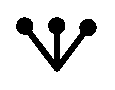
\includegraphics{trees/3_tree.eps}}}}
\newcommand{\ttwor}[1]{#1\tmrsup{\resizebox{0.7em}{!}{
\includegraphics{trees/2r_tree_res.eps}}}}
\newcommand{\tthreer}[1]{#1\tmrsup{\resizebox{0.7em}{!}{
\includegraphics{trees/3r_tree_res.eps}}}}
\newcommand{\tthreeone}[1]{#1^{\resizebox{0.7em}{!}{
\includegraphics{trees/31_tree.eps}}}}
\newcommand{\ttwo}[1]{#1^{\resizebox{0.7em}{!}{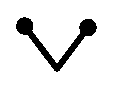
\includegraphics{trees/2_tree.eps}}}}
\newcommand{\tthreethree}[1]{#1\tmrsup{\resizebox{1.1em}{!}{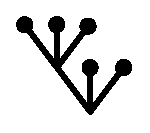
\includegraphics{trees/33_tree.eps}}}}
\newcommand{\tthreetwo}[1]{#1\tmrsup{\resizebox{1.1em}{!}{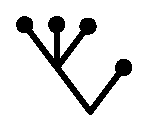
\includegraphics{trees/32_tree.eps}}}}
\newcommand{\tthreethreer}[1]{#1^{\resizebox{1.1em}{!}{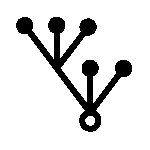
\includegraphics{trees/33_tree_res.eps}}}}
\newcommand{\tthreethreebr}[1]{#1\tmrsup{\resizebox{1.1em}{!}{
\includegraphics{trees/2a1_tree_res.eps}}}}
\newcommand{\ttwoone}[1]{#1^{\resizebox{0.7em}{!}{
\includegraphics{trees/21_tree_mod.eps}}}}
\newcommand{\ttwothreer}[1]{#1^{\resizebox{1.1em}{!}{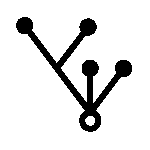
\includegraphics{trees/23_tree_res.eps}}}}
\newcommand{\tthreetwor}[1]{#1^{\resizebox{1.1em}{!}{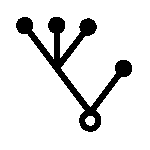
\includegraphics{trees/32_tree_res.eps}}}}
\newcommand{\tone}[1]{#1^{\resizebox{0.3em}{!}{
\includegraphics{trees/1_tree_mod.eps}}}}
\newcommand{\tzero}[1]{#1^{\varnothing}}
\newcommand{\CC}{\mathscr{C} \hspace{.1em}}
\newcommand{\CD}{\mathscr{D} \hspace{.1em}}
\newcommand{\CF}{\mathscr{F} \hspace{.1em}}
\newcommand{\CB}{\mathscr{B} \hspace{.1em}}
\newcommand{\CA}{\mathscr{A} \hspace{.1em}}
\newcommand{\DD}{\mathscr{D} \hspace{.1em}}
\newcommand{\LL}{\mathscr{L} \hspace{.2em}}
\newcommand{\SSS}{S{\hspace{.1em}}}
\newcommand{\PP}{P{\hspace{.1em}}}
\newcommand{\XX}{X}
%

%

\begin{document}

\title{
  Weak universality for a class of\\
  3d stochastic reaction--diffusion models
}

\author{
  M.~Furlan
  \tmaffiliation{CEREMADE\\
  Universit{\'e} Paris Dauphine, France}
  \tmemail{furlan@ceremade.dauphine.fr}
  \and
  M.~Gubinelli
  \tmaffiliation{IAM \& HCM\\
  Universit{\"a}t Bonn, Germany}
  \tmemail{gubinelli@iam.uni-bonn.de}
}

\maketitle

\begin{abstract}
  We establish the large scale convergence of a class of stochastic weakly
  nonlinear reaction--diffusion models on a three dimensional periodic domain
  to the dynamic $\Phi^4_3$ model within the framework of paracontrolled
  distributions. Our work extends previous results of Hairer and Xu to
  nonlinearities with a finite amount of smoothness (in particular $C^9$ is
  enough). We use the Malliavin calculus to perform a partial chaos expansion
  of the stochastic terms and control their $L^p$ norms in terms of the graphs
  of the standard $\Phi^4_3$ stochastic terms. 
\end{abstract}

\tmkeywords{weak universality, paracontrolled distributions, stochastic
quantisation equation, Malliavin calculus, partial chaos expansion.}

\

Consider a family of stochastic reaction--diffusion equation in a
\tmtextit{weakly nonlinear regime}:
\begin{equation}
  \LL u (t, x) = - \varepsilon^{\alpha} F_{\varepsilon} (u (t, x)) + \eta (t,
  x) \label{e:micro} \qquad (t, x) \in [0, T / \varepsilon^2] \times
  (\mathbbm{T}/ \varepsilon)^3
\end{equation}
with $\varepsilon \in (0, 1]$, $T > 0$, initial condition $\bar{u}_{0,
\varepsilon} : (\mathbbm{T}/ \varepsilon)^3 \tmmathbf{} \rightarrow
\mathbbm{R}$, $F_{\varepsilon} \in C^9 (\mathbbm{R})$ with exponential growth
at infinity, $\alpha > 0$ and $\LL : = (\partial_t - \Delta)$ the heat flow
operator and $\mathbbm{T}=\mathbbm{R}/ (2 \pi \mathbbm{Z})$. Here $\eta$ is a
centered Gaussian noise with stationary covariance
\[ \mathbbm{E} (\eta (t, x) \eta (s, y)) = \tilde{C}^{\varepsilon} (t - s, x,
   y) \]
such that $\tilde{C}^{\varepsilon} (t - s, x, y) = \Sigma (t - s, x - y)$ if
$\tmop{dist} (x, y) \leqslant 1$ and $0$ otherwise where $\Sigma : \mathbbm{R}
\times \mathbbm{R}^3 \rightarrow \mathbbm{R}^+$ is a smooth, positive function
compactly supported in $[0, 1] \times B_{\mathbbm{R}^3} (0, 1)$.

We look for a large scale description of the solution to eq.~(\ref{e:micro})
and we introduce the ``mesoscopic'' scale variable $u_{\varepsilon} (t, x) =
\varepsilon^{- \beta} u (t / \varepsilon^2, x / \varepsilon)$ where $\beta >
0$. Substituting $u_{\varepsilon}$ into (\ref{e:micro}) we get
\begin{equation}
  \LL u_{\varepsilon} (t, x) = - \varepsilon^{\alpha - 2 - \beta}
  F_{\varepsilon} (\varepsilon^{\beta} u_{\varepsilon} (t, x)) +
  \varepsilon^{- 2 - \beta} \eta \left( \frac{t}{\varepsilon^2},
  \frac{x}{\varepsilon} \right) . \label{e:micro-2}
\end{equation}
In order for the term $\varepsilon^{- 2 - \beta} \eta (t / \varepsilon^2, x /
\varepsilon)$ to converge to a non--trivial random limit we need that $\beta =
1 / 2$. Indeed the Gaussian field $\eta_{\varepsilon} (t, x) : =
\varepsilon^{- 5 / 2} \eta (t / \varepsilon^2, x / \varepsilon)$ has
covariance $\tilde{C}_{\varepsilon} (t, x) = \varepsilon^{- 5}
\tilde{C}^{\varepsilon} (t / \varepsilon^2, x / \varepsilon)$ and converges in
distribution to the space-time white noise on $\mathbbm{R} \times
\mathbbm{T}^3$. For large values of $\alpha$ the non--linearity will be
negligible with respect to the additive noise term. Heuristically, we can
attempt an expansion of the reaction term around the stationary solution
$Y_{\varepsilon}$ to the linear equation
\[ \LL Y_{\varepsilon} = - Y_{\varepsilon} + \eta_{\varepsilon} . \]
Let us denote with $C_{Y, \varepsilon}$ the covariance of $Y_{\varepsilon}$.
We approximate the reaction term as
\[ \varepsilon^{\alpha - 5 / 2} F_{\varepsilon} (\varepsilon^{1 / 2}
   u_{\varepsilon} (t, x)) \simeq \varepsilon^{\alpha - 5 / 2} F_{\varepsilon}
   (\varepsilon^{1 / 2} Y_{\varepsilon} (t, x)) . \]
The Gaussian r.v. $\varepsilon^{1 / 2} Y_{\varepsilon} (t, x)$ has variance
$\sigma^2_{Y, \varepsilon} = \varepsilon \mathbbm{E} [ (Y_{\varepsilon} (t,
x))^2] = \varepsilon \mathbbm{E} [ (Y_{\varepsilon} (0, 0))^2] = \varepsilon
C_{Y, \varepsilon} (0, 0)$ independent of $(t, x)$. Therefore we can expand
the r.v. $F_{\varepsilon} (\varepsilon^{1 / 2} Y_{\varepsilon} (t, x))$
according to the chaos decomposition relative to $\varepsilon^{1 / 2}
Y_{\varepsilon} (t, x)$ and obtain
\[ F_{\varepsilon} (\varepsilon^{1 / 2} Y_{\varepsilon} (t, x)) = \sum_{n
   \geqslant 0} f_{n, \varepsilon} H_n (\varepsilon^{1 / 2} Y_{\varepsilon}
   (t, x), \sigma^2_{Y, \varepsilon}), \]
where $H_n (x, \sigma^2_{Y, \varepsilon})$ are standard Hermite polynomials
with variance $\sigma^2_{Y, \varepsilon}$. Note that also the coefficients
$(f_{n, \varepsilon})_{n \geqslant 0}$ do not depend on $(t, x)$ by
stationarity of the law of $\varepsilon^{1 / 2} Y_{\varepsilon} (t, x)$ since
they are given by the formula
\[ f_{n, \varepsilon} = n!\mathbbm{E} [F_{\varepsilon} (\varepsilon^{1 / 2}
   Y_{\varepsilon} (t, x)) H_n (\varepsilon^{1 / 2} Y_{\varepsilon} (t, x),
   \sigma_{Y, \varepsilon}^2)] = n!\mathbbm{E} [F_{\varepsilon} (\sigma_{Y,
   \varepsilon} G) H_n (\sigma_{Y, \varepsilon} G, \sigma_{Y, \varepsilon}^2)]
\]
where $G$ is a standard Gaussian variable of unit variance. Let $X$ be the
stationary solution to the equation
\[ \LL X = - X + \xi \]
with $\xi$ the space--time white noise and denote by $\llbracket X^N
\rrbracket$ is the generalized random fields given by the $N$-th Wick power of
$X$ which are well defined as random elements of $\mathcal{S}' (\mathbbm{R}
\times \mathbbm{T}^3)$ as long as $N \leqslant 4$. Denote with $C_X$ the
covariance of $X$. The Gaussian analysis which we set up in this paper shows
in particular the following convergence result.

\begin{theorem}
  \label{th:gaussianAnalysis}Fix $N \leqslant 4$ and assume that
  $\varepsilon^{(n - N) / 2} f_{n, \varepsilon} \rightarrow g_n$ for $0
  \leqslant n \leqslant N$ as $\varepsilon \rightarrow 0$, that
  $(F_{\varepsilon})_{\varepsilon} \subseteq C^{N + 1} (\mathbbm{R})$ and
  there exists constants $c, C > 0$ such that
  \[ \sup_{\varepsilon, x} \sum_{k = 0}^{N + 1} | \partial_x^k F_{\varepsilon}
     (x) | \leqslant C e^{c | x |} . \]
  Then the family of random fields
  \[ \mathbbm{F}^N_{\varepsilon} : (t, x) \mapsto \varepsilon^{- N / 2}
     F_{\varepsilon} (\varepsilon^{1 / 2} Y_{\varepsilon} (t, x)), \qquad (t,
     x) \in \mathbbm{R} \times \mathbbm{T}^3, \]
  converges in law in $\mathcal{S}' (\mathbbm{R} \times \mathbbm{T}^3)$ as
  $\varepsilon \rightarrow 0$ to $\sum_{n = 0}^N g_n \llbracket X^N
  \rrbracket$.
\end{theorem}

Now take the smallest $n$ such that $f_{n, \varepsilon}$ converges to a finite
limit as $\varepsilon \rightarrow 0$. Since $H_n (\varepsilon^{1 / 2}
Y_{\varepsilon}, \sigma_{Y, \varepsilon}^2) = \varepsilon^{n / 2} \llbracket
Y_{\varepsilon}^n \rrbracket$, the $n$-th term in the expansion of
$F_{\varepsilon} (\varepsilon^{1 / 2} Y_{\varepsilon})$ is $f_{n, \varepsilon}
\varepsilon^{\alpha + (n - 5) / 2} \llbracket Y_{\varepsilon}^n \rrbracket$.
From Theorem~\ref{th:gaussianAnalysis} the equation yields a non-trivial limit
only if $\alpha = (5 - n) / 2$. We are interested mainly in the case $n = 3
\Rightarrow \alpha = 1$ and $n = 1 \Rightarrow \alpha = 2$. The case $\alpha =
2$ gives rise to a Gaussian limit and its analysis its not very difficult.

In the following we will concentrate in the analysis of the $\alpha = 1$ case
where the limiting behaviour of the model is the most interesting and given by
the $\Phi^4_3$ family of singular SPDEs. In this case we obtain the family of
models
\begin{equation}
  \LL u_{\varepsilon} (t, x) = - \varepsilon^{- \frac{3}{2}} F_{\varepsilon}
  (\varepsilon^{\frac{1}{2}} u_{\varepsilon} (t, x)) + \eta_{\varepsilon} (t,
  x) \quad \label{e:univ}
\end{equation}
with initial condition $u_{0, \varepsilon} (\cdummy) \assign \varepsilon^{-
\frac{1}{2}} \bar{u}_{0, \varepsilon} (\varepsilon^{- 1} \cdummy)$ where
$\bar{u}_{0, \varepsilon}$ is the initial condition of the microscopic
model~(\ref{e:micro}). \

Define for $m \geqslant 0$ and $\zeta = (t, x) \in \mathbbm{R}^+ \times
\mathbbm{T}^3$
\begin{equation}
  \Phi_{\zeta}^{(m)} \assign \varepsilon^{(m - 3) / 2}
  \tilde{F}_{\varepsilon}^{ (m)} (\varepsilon^{1 / 2} Y_{\varepsilon, \zeta})
  . \label{e:def-phi}
\end{equation}
where $\tilde{F}_{\varepsilon}$ is the centered function
\[ \tilde{F}_{\varepsilon}  (x) \assign F_{\varepsilon} (x) - f_{0,
   \varepsilon} - f_{1, \varepsilon} x - f_{2, \varepsilon} H_2 (x, \sigma_{Y,
   \varepsilon}^2) = \sum_{n \geqslant 3} f_{n, \varepsilon} H_n (x,
   \sigma_{Y, \varepsilon}^2), \]
and $\sigma_{Y, \varepsilon}^2$ is the variance of the centered Gaussian
process $\varepsilon^{1 / 2} Y_{\varepsilon}$. Note that $H_n (\varepsilon^{1
/ 2} Y_{\varepsilon} (\cdot), \sigma_{Y, \varepsilon}^2) = \varepsilon^{n / 2}
\llbracket Y^n_{\varepsilon} \rrbracket$ and denote with $f_{n, \varepsilon}$
the coefficients in the chaos expansion of $F_{\varepsilon}^{} (\varepsilon^{1
/ 2} Y_{\varepsilon, \zeta})$. Define also various $\varepsilon$--dependent
constants
\begin{equation}
  \begin{array}{rclcrcl}
    \ttwothreer{d_{\varepsilon}} & \assign & \frac{1}{9} \int_{s, x} P_s (x)
    \mathbbm{E} [\Phi^{(1)}_0 \Phi^{(1)}_{(s, x)}], & \qquad &
    \ttwothreer{\tilde{d}_{\varepsilon}} & \assign & 2 \varepsilon^{- 1 / 2}
    f_{3, \varepsilon} f_{2, \varepsilon}  \int_{s, x} P_s (x) [C_{Y,
    \varepsilon} (s, x)]^2,\\
    \tthreetwor{d_{\varepsilon}} & \assign & \frac{1}{6} \int_{s, x} P_s (x)
    \mathbbm{E} [\Phi^{(0)}_0 \Phi^{(2)}_{(s, x)}], &  &
    \tthreethreer{\hat{d}_{\varepsilon}} & \assign & \frac{1}{3} \int_{s, x}
    P_s (x) \mathbbm{E} [\Phi^{(0)}_0 \Phi^{(1)}_{(s, x)}],\\
    \tthreethreer{d_{\varepsilon}} & \assign & 2 \tthreetwor{d_{\varepsilon}}
    + 3 \ttwothreer{d_{\varepsilon}} &  &  &  & 
  \end{array} \label{eq:d-constants}
\end{equation}
where $P_s (x)$ is the heat kernel and $\int_{s, x}$ denotes integration on
$\mathbbm{R}^+ \times \mathbbm{T}^3$.

\begin{axiom}
  \label{a:main}All along the paper we enforce the following assumptions:
  \begin{enumeratealpha}
    \item $(u_{0, \varepsilon})_{\varepsilon}$ converges to a limit $u_0$ in
    $\CC^{- 1 / 2 - \kappa}$ and is independent of $\eta$;
    
    \item $(\bar{u}_{0, \varepsilon})_{\varepsilon}$ is uniformly bounded in
    $L^{\infty}$, i.e. $\exists C > 0$ such that $\forall \varepsilon \in (0,
    1]$ $\| \bar{u}_{0, \varepsilon} \|_{L^{\infty} ((\mathbbm{T}/
    \varepsilon)^3)} \leqslant C$;
    
    \item $(F_{\varepsilon})_{\varepsilon} \subseteq C^9 (\mathbbm{R})$ and
    there exists constants $c, C > 0$ such that
    \begin{equation}
      \sup_{\varepsilon, x} \sum_{k = 0}^9 | \partial_x^k F_{\varepsilon} (x)
      | \leqslant C e^{c | x |}, \label{e:hyp-F-main}
    \end{equation}
    \item the vectors $\lambda_{\varepsilon} = (\lambda_{\varepsilon}^{(0)},
    \lambda_{\varepsilon}^{(1)}, \lambda_{\varepsilon}^{(2)},
    \lambda_{\varepsilon}^{(3)}) \in \mathbbm{R}^4$ given by
    \begin{equation}
      \begin{array}{rclcrcl}
        \lambda^{(3)}_{\varepsilon} & = & f_{3, \varepsilon} &  &
        \lambda^{(1)}_{\varepsilon} & = & \varepsilon^{- 1} f_{1, \varepsilon}
        - 3 \tthreethreer{d_{\varepsilon}}\\
        \lambda_{\varepsilon}^{(2)} & = & \varepsilon^{- 1 / 2} f_{2,
        \varepsilon} &  & \lambda_{\varepsilon}^{(0)} & = & \varepsilon^{- 3 /
        2} f_{0, \varepsilon} - \varepsilon^{- 1 / 2} f_{2, \varepsilon} 
        \tthreetwor{d_{\varepsilon}} - 3 \ttwothreer{\tilde{d}_{\varepsilon}}
        - 3 \tthreethreer{\hat{d}_{\varepsilon}}
      \end{array} \label{e:def-lambda}
    \end{equation}
    have a finite limit $\lambda = (\lambda^{(0)}, \lambda^{(1)},
    \lambda^{(2)}, \lambda^{(3)}) \in \mathbbm{R}^4$ as $\varepsilon
    \rightarrow 0$. 
  \end{enumeratealpha}
\end{axiom}

We can now formulate our main result.

\begin{theorem}
  \label{t:maintheorem}Under Assumptions~\ref{a:main} the family of random
  fields $(u_{\varepsilon})_{\varepsilon}$ given by the solution to
  eq.~(\ref{e:univ}) converge in law and locally in time to a limiting random
  field $u (\lambda)$ in the space $C_T \CC^{- \alpha} (\mathbbm{T}^3)$ for
  every $1 / 2 < \alpha < 2 / 3$. The law of $u (\lambda)$ depends only on the
  value of $\lambda$ and not on the other details of the nonlinearity or on
  the covariance of the noise term. We call this limit the dynamic $\Phi^4_3$
  model with parameter vector $\lambda \in \mathbbm{R}^4$. \ 
\end{theorem}

Here $C_T \CC^{- \alpha} (\mathbbm{T}^3)$ denotes the space of continuous
functions from $[0, T]$ to the Besov space $\CC^{- \alpha} (\mathbbm{T}^3) =
B^{- \alpha}_{\infty, \infty} (\mathbbm{T}^3)$ (see Appendix~\ref{a:basics}
for details).

\begin{remark}
  \label{r:usualphi4}In particular we can take
  \[ \begin{array}{lll}
       F_{\varepsilon} (x) & = & \sigma^{(3)} H_3 (x, \sigma_{Y,
       \varepsilon}^2) + \varepsilon^{1 / 2} \sigma^{(2)} H_2 (x, \sigma_{Y,
       \varepsilon}^2) + \varepsilon (\sigma^{(1)} +
       \gamma^{(1)}_{\varepsilon}) H_1 (x, \sigma_{Y, \varepsilon}^2) +
       \varepsilon^{3 / 2} (\sigma^{(0)} + \gamma^{(0)}_{\varepsilon})
     \end{array} \]
  so that
  \[ f_{3, \varepsilon} = \sigma^{(3)}, \quad \varepsilon^{- 1 / 2} f_{2,
     \varepsilon} = \sigma^{(2)}, \quad \varepsilon^{- 1} f_{1, \varepsilon} =
     \sigma^{(1)} + \gamma^{(1)}_{\varepsilon}, \quad \varepsilon^{- 3 / 2}
     f_{0, \varepsilon} = \sigma^{(0)} + \gamma_{\varepsilon}^{(0)}, \]
  and
  \[ \tthreethreer{d_{\varepsilon}} = 3 (\sigma^{(3)})^2 L_{\varepsilon},
     \quad \ttwothreer{\tilde{d}_{\varepsilon}} = \sigma^{(3)} \sigma^{(2)}
     L_{\varepsilon}, \quad \tthreetwor{d_{\varepsilon}} =
     \tthreethreer{\hat{d}_{\varepsilon}} = 0, \]
  where $L_{\varepsilon} \assign 2 \int_{s, x} P_s (x) (C_{Y, \varepsilon} (s,
  x))^2 .$ Choosing
  \[ \gamma^{(1)}_{\varepsilon} \assign 3 \tthreethreer{d_{\varepsilon}} = 9
     (\sigma^{(3)})^2 L_{\varepsilon}, \qquad \gamma^{(0)}_{\varepsilon}
     \assign 3 \ttwothreer{\tilde{d}_{\varepsilon}} = 3 \sigma^{(3)}
     \sigma^{(2)} L_{\varepsilon}, \]
  we obtain $\lambda_{\varepsilon} \rightarrow (\sigma^{(0)}, \sigma^{(1)},
  \sigma^{(2)}, \sigma^{(3)})$. This shows that all the possible limits
  $\lambda \in \mathbbm{R}^4$ are attainable. In this case (\ref{e:univ})
  takes the form
  \begin{equation}
    \LL u_{\varepsilon} = - \sigma^{(3)} u_{\varepsilon}^3 - \sigma^{(2)}
    u_{\varepsilon}^2 - [\sigma^{(1)} - 3 \sigma^{(3)} \varepsilon^{- 1}
    \sigma^2_{Y, \varepsilon} + 9 (\sigma^{(3)})^2 L_{\varepsilon}]
    u_{\varepsilon} - \sigma^{(0)} + \sigma^{(2)} \sigma^2_{Y, \varepsilon} -
    3 \sigma^{(3)} \sigma^{(2)} L_{\varepsilon} + \eta_{\varepsilon} .
    \label{eq:cubic}
  \end{equation}
\end{remark}

When the nonlinearity is given by a cubic polynomial like in~(\ref{eq:cubic})
the corresponding limiting model is called dynamic $\Phi^4_3$ equation or
stochastic quantisation equation. In two dimensions, this model has been
subject of various studies since more than thirty
years~{\cite{jona-lasinio_stochastic_1985,albeverio_stochastic_1991,da_prato_strong_2003}}.
For the three dimensional case, the kind of convergence results described
above are originally due to
Hairer~{\cite{hairer_theory_2014,hairer_regularity_2015}} and constitute one
of the first groundbreaking applications of his theory of regularity
structures. Similar results were later obtained by Catellier and
Chouk~{\cite{catellier_paracontrolled_2013}} using the paracontrolled approach
of Gubinelli, Imkeller and Perkowski~{\cite{gubinelli_paracontrolled_2012}}.
Kupiainen~{\cite{kupiainen_renormalization_2014}} described a third approach
using renormalization group ideas.

\tmtextit{Weak universality} is the observation that the same limiting object
describes the large scale behaviour of the solutions of more general
equations, in particular that of the many parameters present in a general
model, only a finite number of their combinations survive in the limit to
describe the limiting object. The adjective ``weak'' is related to the fact
that in order to control the large scale limit the non-linearity has to be
very small in the microscopic scale. This sets up a perturbative regime which
is well suited to the analysis via regularity structures or paracontrolled
distributions.

The first result of weak universality for a singular stochastic PDE has been
given by Hairer and Quastel~{\cite{hairer_class_2015}} in the context the
Kardar--Parisi--Zhang equation. Using the machinery developed there Hairer and
Wu~{\cite{hairer_large_2016}} proved a weak universality result for three
dimensional reaction--diffusion equations in the case of Gaussian noise and a
polynomial non--linearity, within the context of regularity structures. Weak
universality for reaction--diffusion equations driven by non Gaussian noise is
analysed in Shen and Wu~{\cite{shen_weak_2016}}. Recently, important results
concerning the stochastic quantisation equation we obtained by Mourrat and
Weber. In particular the convergence to the dynamic $\Phi^4_2$ model for a
class of Markovian dynamics of discrete spin
systems~{\cite{mourrat_convergence_2014}} and also the global wellposedness of
$\Phi^4_2$ in space and time~{\cite{mourrat_global_2015}} and in time for
$\Phi^4_3$~{\cite{mourrat_global_2016}}. The recent
preprint~{\cite{gubinelli_renormalization_2017}} analyzes an hyperbolic version
of the stochastic quantisation equation in two dimensions, including the
associated universality in the small noise regime.

The present work is the first which considers in detail the weak universality
problem in the context of paracontrolled distributions, showing that on the
analytic side the apriori estimates can be obtained via standard arguments and
that the major difficulty is related to showing the convergence of a finite
number of random fields to universal limiting objects. The main point of our
analysis is our use of the Malliavin
calculus~{\cite{nualart_2006,nourdin_peccati_2012}} to perform the analysis of
these stochastic terms without requiring polynomial non--linearity as in the
previous works cited above. In particular we were inspired by the computations
in~{\cite{nourdin_nualart_2007}} and in general by the use of the Malliavin
calculus to establish normal approximations~{\cite{nourdin_peccati_2012}}. The
main technical results of our paper, Theorem~\ref{t:stoch-conv} below, is not
particularly linked to paracontrolled distributions. A similar analysis is
conceivable \ for the stochastic models in regularity structures. Moreover the
same tools can also allow to prove similar non-polynomial weak universality
statements for the KPZ along the lines of the present analysis. This is the
subject of ongoing work.

\

The paper is structured as follows. Section~\ref{s:universal-analytic}
contains the paracontrolled analysis of eq.~(\ref{e:univ}) which will allow to
obtain uniform estimates to pass to the limit. Section~\ref{s:comparing} in
the core of the paper, it contains the stochastic analysis based on Malliavin
calculus which allows to control the limit of the random fields involved in
the paracontrolled description of eq.~(\ref{e:univ}) and to identify their
limits. All the rest of the paper consists in three appendices which do not
contain original material but allow the paper to be self contained. In
particular Appendix~\ref{a:basics} collects notations and basic results of
paracontrolled calculus. Appendix~\ref{a:malliavin} collects basic definitions
and results from Malliavin calculus which will be needed in the analysis of
the stochastic terms. Finally Appendix~\ref{a:ker-est} contains mostly some
technical estimates on kernels needed in the stochastic analysis. The reader
not familiar with paracontrolled calculus and/or Malliavin calculus is
encouraged to read Appendix~\ref{a:basics} and/or Appendix~\ref{a:malliavin}
before going on. In particular please refer to Section~\ref{s:notations} for
the notations and conventions in force all along the paper.

\section{\label{s:universal-analytic}Analysis of the mesoscopic model}

In this section we describe the paracontrolled
approach~{\cite{gubinelli_paracontrolled_2012}} to a solution theory for
eq.~(\ref{e:univ}) along the lines of the
Catellier--Chouk~{\cite{catellier_paracontrolled_2013}} analysis. The basic
results of paracontrolled calculus we need in this section are included in
Appendix~\ref{a:basics}.

The continuity of the solution map for a paracontrolled equation (already
established in~{\cite{catellier_paracontrolled_2013}} and recalled here)
allows us to prove convergence of the solution $u_{\varepsilon}$
(Theorem~\ref{t:maintheorem}) by showing the convergence of the enhanced noise
$\mathbbm{Y}_{\varepsilon}$ and the remainder $R_{\varepsilon}$ in the
appropriate space. Finally, in Theorem~\ref{t:lim-ident} we identify the
limiting process as the solution of a paracontrolled equation.

\subsection{Paracontrolled structure}

Write $u_{\varepsilon} = Y_{\varepsilon} + v_{\varepsilon}$, and perform a
Taylor expansion of the reaction term $\tilde{F}_{\varepsilon} (\varepsilon^{1
/ 2} Y_{\varepsilon} + \varepsilon^{1 / 2} v_{\varepsilon})$ in (\ref{e:univ})
around $\varepsilon^{1 / 2} Y_{\varepsilon}$ up to the third order to get
\begin{equation}
  \begin{array}{lll}
    \LL u_{\varepsilon} & = & \eta_{\varepsilon} - \Phi^{(0)} - \Phi^{(1)}
    v_{\varepsilon} - \frac{1}{2} \Phi^{(2)} v_{\varepsilon}^2 - \frac{1}{6}
    \Phi^{(3)} v_{\varepsilon}^3 - R_{\varepsilon} (v_{\varepsilon})\\
    &  & - \varepsilon^{- 3 / 2} f_{0, \varepsilon} - \varepsilon^{- 1} f_{1,
    \varepsilon} (Y_{\varepsilon} + v_{\varepsilon}) - \varepsilon^{- 1 / 2}
    f_{2, \varepsilon} (\llbracket Y_{\varepsilon}^2 \rrbracket + 2
    v_{\varepsilon} Y_{\varepsilon} + v_{\varepsilon}^2) .
  \end{array} \label{eq:first-exp}
\end{equation}
with $\Phi_{\zeta}^{(m)}$ defined in (\ref{e:def-phi}) $\forall \zeta \in
\mathbbm{R} \times \mathbbm{T}^3$ and $R_{\varepsilon} (v_{\varepsilon})$ the
remainder of the Taylor series.

Define the following random fields:
\begin{equation}
  \begin{array}{lclclcl}
    \LL Y_{\varepsilon} & \assign & \eta_{\varepsilon} & \hspace{4em} &
    \ttwo{\tilde{Y}_{\varepsilon}} & \assign & \varepsilon^{- 1 / 2} f_{2,
    \varepsilon}  \llbracket Y_{\varepsilon}^2 \rrbracket,\\
    \LL \tthreeone{Y_{\varepsilon}} & \assign & \Phi^{(0)}, &  &
    \tthreetwor{Y_{\varepsilon}} & \assign & \tthreeone{Y_{\varepsilon}} \circ
    \tone{Y_{\varepsilon}} - \tthreetwor{d_{\varepsilon}},\\
    \ttwo{Y_{\varepsilon}} & \assign & \frac{1}{3} \Phi^{(1)} &  &
    \tthreethreer{Y_{\varepsilon}} & \assign & \tthreeone{Y_{\varepsilon}}
    \circ \ttwo{Y_{\varepsilon}} - \tthreethreer{d_{\varepsilon}}
    Y_{\varepsilon} - \tthreethreer{\hat{d}_{\varepsilon}},\\
    \LL \ttwoone{Y_{\varepsilon}} & \assign & \ttwo{Y_{\varepsilon}}, &  &
    \ttwothreer{Y_{\varepsilon}} & \assign & \ttwoone{Y_{\varepsilon}} \circ
    \ttwo{Y_{\varepsilon}} - \ttwothreer{d_{\varepsilon}},\\
    \tone{Y_{\varepsilon}} & \assign & \frac{1}{6} \Phi^{(2)}, &  &
    \ttwothreer{\tilde{Y}_{\varepsilon}} & \assign &
    \ttwoone{\tilde{Y}_{\varepsilon}} \circ \ttwo{Y_{\varepsilon}} -
    \ttwothreer{\tilde{d}_{\varepsilon}},\\
    \tzero{Y_{\varepsilon}} & \assign & \frac{1}{6} \Phi^{(3)}, &  &  &  & 
  \end{array} \label{e:trees-def}
\end{equation}
with $\Phi^{(m)}$ defined in (\ref{e:def-phi}) and $Y_{\varepsilon},
\tthreeone{Y_{\varepsilon}}, \ttwoone{Y_{\varepsilon}}$ stationary solutions.
In the scope of this section we can take any constants
$d_{\varepsilon}^{\tau}$ that satisfy
\begin{equation}
  \begin{array}{lll}
    \tthreethreer{d_{\varepsilon}} & = & 2 \tthreetwor{d_{\varepsilon}} + 3
    \ttwothreer{d_{\varepsilon}} .
  \end{array} \label{e:ren-constraint}
\end{equation}
Equation~(\ref{eq:first-exp}) takes the form
\begin{equation}
  \begin{array}{lll}
    \LL v_{\varepsilon} & = & Y_{\varepsilon} - \tthree{Y_{\varepsilon}} -
    \ttwo{\tilde{Y}_{\varepsilon}} - 3 \ttwo{Y_{\varepsilon}} v_{\varepsilon}
    - 3 \tone{Y_{\varepsilon}} v_{\varepsilon}^2 - \tzero{Y_{\varepsilon}}
    v_{\varepsilon}^3\\
    &  & - \varepsilon^{- 3 / 2} f_{0, \varepsilon} - \varepsilon^{- 1} f_{1,
    \varepsilon}  (Y_{\varepsilon} + v_{\varepsilon}) - \varepsilon^{- 1 / 2}
    f_{2, \varepsilon}  (2 Y_{\varepsilon} v_{\varepsilon} +
    v_{\varepsilon}^2) - R_{\varepsilon} (v_{\varepsilon}) .
  \end{array} \label{eq1}
\end{equation}
In this expression the products $\ttwo{Y_{\varepsilon}} v_{\varepsilon}$,
$\tone{Y_{\varepsilon}} v_{\varepsilon}^2$ and $Y_{\varepsilon}
v_{\varepsilon}$ do not meet the conditions for continuity. In order to
continue the analysis we pose the paracontrolled Ansatz
\begin{equation}
  v_{\varepsilon} = - \tthreeone{Y_{\varepsilon}} -
  \ttwoone{\tilde{Y}_{\varepsilon}} - 3 v_{\varepsilon} \precprec
  \ttwoone{Y_{\varepsilon}} + v^{\sharp}_{\varepsilon}, \quad
  \label{e:ansatz-univ}
\end{equation}
and proceed to decompose the ill-defined products using the paracontrolled
techniques recalled in Appendix~\ref{a:basics} . We start with
\[ v_{\varepsilon} \ttwo{Y_{\varepsilon}} = v_{\varepsilon} \prec
   \ttwo{Y_{\varepsilon}} + v_{\varepsilon} \succ \ttwo{Y_{\varepsilon}} +
   v_{\varepsilon} \circ \ttwo{Y_{\varepsilon}} . \]
The resonant term, together with Ansatz~(\ref{e:ansatz-univ}), yields:
\begin{eqnarray*}
  v_{\varepsilon} \circ \ttwo{Y_{\varepsilon}} & = & -
  \tthreeone{Y_{\varepsilon}} \circ \ttwo{Y_{\varepsilon}} -
  \ttwoone{\tilde{Y}_{\varepsilon}} \circ \ttwo{Y_{\varepsilon}} - 3
  v_{\varepsilon}  (\ttwoone{Y_{\varepsilon}} \circ \ttwo{Y_{\varepsilon}})
  %\\ &  & 
  - 3 \overline{\tmop{com}}_1 (v_{\varepsilon},
  \ttwoone{Y_{\varepsilon}}, \ttwo{Y_{\varepsilon}}) +
  v^{\sharp}_{\varepsilon} \circ \ttwo{Y_{\varepsilon}} .
\end{eqnarray*}
So we let
\[ \begin{array}{lll}
     \ttwo{Y_{\varepsilon}} \hat{\diamond} v_{\varepsilon} & \assign &
     v_{\varepsilon} \ttwo{Y_{\varepsilon}} - v_{\varepsilon} \prec
     \ttwo{Y_{\varepsilon}} + (3 v_{\varepsilon}  \ttwothreer{d_{\varepsilon}}
     + \tthreethreer{d_{\varepsilon}} Y_{\varepsilon} +
     \tthreethreer{\hat{d}_{\varepsilon}} +
     \ttwothreer{\tilde{d}_{\varepsilon}})\\
     & = & v_{\varepsilon} \succ \ttwo{Y_{\varepsilon}} -
     \ttwothreer{\tilde{Y}_{\varepsilon}} - \tthreethreer{Y_{\varepsilon}} - 3
     v_{\varepsilon}  \ttwothreer{Y_{\varepsilon}} + v^{\sharp}_{\varepsilon}
     \circ \ttwo{Y_{\varepsilon}} - 3 \overline{\tmop{com}}_1
     (v_{\varepsilon}, \ttwoone{Y_{\varepsilon}}, \ttwo{Y_{\varepsilon}})
   \end{array} \]
Moreover we have for $v_{\varepsilon} Y_{\varepsilon}$:
\[ \begin{array}{lll}
     v_{\varepsilon} Y_{\varepsilon} & = & \varphi_{\varepsilon}
     Y_{\varepsilon} - \tthreeone{Y_{\varepsilon}} \prec Y_{\varepsilon} -
     \tthreeone{Y_{\varepsilon}} \succ Y_{\varepsilon} -
     \tthreeone{Y_{\varepsilon}} \circ Y_{\varepsilon}
   \end{array} \]
where we introduced the shorthand $\varphi_{\varepsilon} = v_{\varepsilon} +
\tthreeone{Y_{\varepsilon}}$. So we let
\[ v_{\varepsilon} \diamond Y_{\varepsilon} \assign v_{\varepsilon}
   Y_{\varepsilon} + \tthreetwor{d_{\varepsilon}} = \varphi_{\varepsilon}
   Y_{\varepsilon} - \tthreeone{Y_{\varepsilon}} \prec Y_{\varepsilon} -
   \tthreeone{Y_{\varepsilon}} \succ Y_{\varepsilon} -
   \tthreetwor{Y_{\varepsilon}} \]
Finally to analyse the product $\tone{Y_{\varepsilon}} v_{\varepsilon}^2$ we
write
\[ \tone{Y_{\varepsilon}} v_{\varepsilon}^2 = \tone{Y_{\varepsilon}}
   (\tthreeone{Y_{\varepsilon}})^2 - 2 \tone{Y_{\varepsilon}}
   \tthreeone{Y_{\varepsilon}} \varphi_{\varepsilon} + \tone{Y_{\varepsilon}}
   \varphi_{\varepsilon}^2, \]
and consider the products involving only $Y^{\tau}$ factors: first
\[ \tone{Y_{\varepsilon}} \tthreeone{Y_{\varepsilon}} = \tone{Y_{\varepsilon}}
   \succ \tthreeone{Y_{\varepsilon}} + \tone{Y_{\varepsilon}} \prec
   \tthreeone{Y_{\varepsilon}} + \tthreetwor{Y_{\varepsilon}} +
   \tthreetwor{d_{\varepsilon}} = : \tone{Y_{\varepsilon}} \diamond
   \tthreeone{Y_{\varepsilon}} + \tthreetwor{d_{\varepsilon}}, \]
and then we define the term $\tone{Y_{\varepsilon}} \diamond
(\tthreeone{Y_{\varepsilon}})^2$ as follows:
\begin{eqnarray*}
  \tone{Y_{\varepsilon}} \diamond (\tthreeone{Y_{\varepsilon}})^2 & \assign &
  \tone{Y_{\varepsilon}} (\tthreeone{Y_{\varepsilon}})^2 - 2
  \tthreetwor{d_{\varepsilon}} \tthreeone{Y_{\varepsilon}}\\
  & = & \tone{Y_{\varepsilon}} \prec (\tthreeone{Y_{\varepsilon}})^2 +
  \tone{Y_{\varepsilon}} \succ (\tthreeone{Y_{\varepsilon}})^2 +
  \tone{Y_{\varepsilon}} \circ (\tthreeone{Y_{\varepsilon}} \circ
  \tthreeone{Y_{\varepsilon}}) + 2 \tmop{com}_1 (\tthreeone{Y_{\varepsilon}},
  \tthreeone{Y_{\varepsilon}}, \tone{Y_{\varepsilon}}) + 2
  \tthreeone{Y_{\varepsilon}} \tthreetwor{Y_{\varepsilon}} .
\end{eqnarray*}
so that
\[ \tone{Y_{\varepsilon}} \diamond v_{\varepsilon}^2 \assign
   \tone{Y_{\varepsilon}} v_{\varepsilon}^2 + 2 \tthreetwor{d_{\varepsilon}}
   v_{\varepsilon} = \tone{Y_{\varepsilon}} \diamond
   (\tthreeone{Y_{\varepsilon}})^2 - 2 (\tone{Y_{\varepsilon}} \diamond
   \tthreeone{Y_{\varepsilon}}) \varphi_{\varepsilon} + \tone{Y_{\varepsilon}}
   \varphi_{\varepsilon}^2 \]
We note also that
\[ \LL v_{\varepsilon} = - \LL \tthreeone{Y_{\varepsilon}} - \LL
   \ttwoone{\tilde{Y}_{\varepsilon}} + \LL v^{\sharp}_{\varepsilon} - 3
   v_{\varepsilon} \prec \LL \ttwoone{Y_{\varepsilon}} - 3 \tmop{com}_3
   (v_{\varepsilon}, \ttwoone{Y_{\varepsilon}}) - 3 \tmop{com}_2
   (v_{\varepsilon}, \ttwo{Y_{\varepsilon}}) . \]
Substituting these renormalized products into (\ref{eq1}) we obtain the
following equation for $v^{\sharp}_{\varepsilon}$ :
\begin{eqnarray}
  \LL v_{\varepsilon}^{\sharp} & = & 3 \tmop{com}_3 (v_{\varepsilon},
  \ttwoone{Y_{\varepsilon}}) + 3 \tmop{com}_2 (v_{\varepsilon},
  \ttwo{Y_{\varepsilon}}) \nonumber\\
  &  & - \tzero{Y_{\varepsilon}} v_{\varepsilon}^3 - 3 \tone{Y_{\varepsilon}}
  \diamond v_{\varepsilon}^2 - 3 \ttwo{Y_{\varepsilon}} \hat{\diamond}
  v_{\varepsilon} \nonumber\\
  &  & + Y_{\varepsilon} - \lambda_{\varepsilon}^{(2)} (2 v_{\varepsilon}
  \diamond Y_{\varepsilon} + v_{\varepsilon}^2) \nonumber\\
  &  & - \lambda^{(1)}_{\varepsilon}  (Y_{\varepsilon} + v_{\varepsilon}) +
  [9 \ttwothreer{d_{\varepsilon}} + 6 \tthreetwor{d_{\varepsilon}} - 3
  \tthreethreer{d_{\varepsilon}}] v_{\varepsilon} -
  \lambda_{\varepsilon}^{(0)} - R_{\varepsilon} (v_{\varepsilon}) \nonumber\\
  & = & U (\lambda_{\varepsilon}, \mathbbm{Y}_{\varepsilon} ;
  v_{\varepsilon}, v_{\varepsilon}^{\sharp}) - R_{\varepsilon}
  (v_{\varepsilon})  \label{e:last-phisharp}
\end{eqnarray}
with $R_{\varepsilon} (v_{\varepsilon})$ the Taylor remainder which appears
in~(\ref{eq:first-exp}) and $\lambda_{\varepsilon} =
(\lambda_{\varepsilon}^{(0)}, \lambda_{\varepsilon}^{(1)},
\lambda_{\varepsilon}^{(2)}, \lambda_{\varepsilon}^{(3)}) \in \mathbbm{R}^4$
given by eq.~(\ref{e:def-lambda}) and where we can use the
constraint~(\ref{e:ren-constraint}) to remove the term proportional to
$v_{\varepsilon}$. The enhanced noise vector $\mathbbm{Y}_{\varepsilon}$ is
defined by
\begin{eqnarray}
  \mathbbm{Y}_{\varepsilon} & \assign & (\tzero{Y_{\varepsilon}},
  \tone{Y_{\varepsilon}}, \ttwo{Y_{\varepsilon}},
  \ttwo{\tilde{Y}_{\varepsilon}}, \tthreeone{Y_{\varepsilon}},
  \tthreetwor{Y_{\varepsilon}}, \ttwothreer{Y_{\varepsilon}},
  \ttwothreer{\tilde{Y}_{\varepsilon}}, \tthreethreer{Y_{\varepsilon}})
  \nonumber\\
  &  &  \nonumber\\
  \mathcal{X}_T & \assign & C_T^{} \CC^{- \kappa} \times C_T \CC^{-
  \frac{1}{2} - \kappa} \times \left( C_T \CC^{- 1 - \kappa} \right)^2 \times
  \LL_T^{1 / 2 - \kappa} \times \left( C_T \CC^{- \kappa} \right)^3 \times C_T
  \CC^{- \frac{1}{2} - \kappa}  \label{e:y-space}
\end{eqnarray}
for every $\kappa > 0$. We use the notation $\| \mathbbm{Y}_{\varepsilon}
\|_{\mathcal{X}_T} = \sum_{\tau} \| \mathbbm{Y}^{\tau}_{\varepsilon}
\|_{\mathcal{X}^{\tau}}$ for the associated norm where
$Y_{\varepsilon}^{\tau}$ is a generic tree in $\mathbbm{Y}_{\varepsilon}$. The
homogeneities $| \tau | \in \mathbbm{R}$ are given by
\[ \begin{array}{|c|c|c|c|c|c|c|c|c|c|c|}
     \hline
     Y_{\varepsilon}^{\tau} & = & \tzero{Y_{\varepsilon}} &
     \tone{Y_{\varepsilon}} & \ttwo{Y_{\varepsilon}} &
     \ttwo{\tilde{Y}_{\varepsilon}} & \tthreeone{Y_{\varepsilon}} &
     \tthreetwor{Y_{\varepsilon}} & \ttwothreer{Y_{\varepsilon}} &
     \ttwothreer{\tilde{Y}_{\varepsilon}} & \tthreethreer{Y_{\varepsilon}}\\
     \hline
     | \tau | & = & 0 & - 1/2 & - 1 & - 1 & 1/2 & 0 & 0 & 0 &
     - 1/2\\
     \hline
   \end{array} \]
Notice that for every $\varepsilon > 0$ eq.~(\ref{e:last-phisharp}) is
equivalent to~(\ref{e:univ}) together with Ansatz~(\ref{e:ansatz-univ}).

\subsection{A-priori estimates}

In this section we show uniform a-priori estimates for the pair
$(v_{\varepsilon}, v^{\flat}_{\varepsilon})$ which solves the following system
of equations
\begin{equation}
  \left\{ \begin{array}{lll}
    v_{\varepsilon} & = & - \tthreeone{Y_{\varepsilon}} -
    \ttwoone{\tilde{Y}_{\varepsilon}} - 3 v_{\varepsilon} \precprec
    \ttwoone{Y_{\varepsilon}} + v^{\flat}_{\varepsilon} +
    v^{\natural}_{\varepsilon}\\
    \LL v_{\varepsilon}^{\flat} & = & U (\lambda_{\varepsilon},
    \mathbbm{Y}_{\varepsilon} ; v_{\varepsilon}, v^{\flat}_{\varepsilon} +
    v^{\natural}_{\varepsilon}) - R_{\varepsilon} (v_{\varepsilon})\\
    v^{\flat}_{\varepsilon} (0) & = & \tthreeone{Y_{\varepsilon}} (0) +
    \ttwoone{\tilde{Y}_{\varepsilon}} (0) + 3 v_{\varepsilon, 0} \prec
    \ttwoone{Y_{\varepsilon}} (0)
  \end{array} \right. \label{e:fixpoint-final}
\end{equation}
with $v^{\natural}_{\varepsilon} (t) \assign P_t v_{\varepsilon, 0}$ and
$v_{\varepsilon, 0} \assign u_{0, \varepsilon} - Y_{\varepsilon} (0) \in
\CC^{- 1 / 2 -}$. $U$ is given in (\ref{e:last-phisharp}). It is easy to see,
by taking $v^{\sharp}_{\varepsilon} = v^{\flat}_{\varepsilon} +
v^{\natural}_{\varepsilon}$, that this is equivalent to
eq.~(\ref{e:last-phisharp}) together with Ansatz~(\ref{e:ansatz-univ}) on
$v_{\varepsilon}$. We consider the spaces
\[ \mathcal{V}_T^{\flat} \assign \LL^{2 \kappa}_T \cap \LL^{1 / 4, 1 / 2 + 2
   \kappa}_T \cap \LL^{1 / 2, 1 + 2 \kappa}_T, \quad \mathcal{V}_T \assign
   \LL^{1 / 2, 1 / 2 - \kappa}_T \cap \LL_T^{1 / 4 + 3 \kappa / 2, 2 \kappa},
\]
with the corresponding norms
\begin{eqnarray}
  \| v^{\flat}_{\varepsilon} \|_{\mathcal{V}_T^{\flat}} & \assign & \|
  v^{\flat}_{\varepsilon} \|_{\LL^{2 \kappa}_T} + \| v^{\flat}_{\varepsilon}
  \|_{\LL^{1 / 4, 1 / 2 + 2 \kappa}_T} + \| v_{\varepsilon}^{\flat} \|_{\LL^{1
  / 2, 1 + 2 \kappa}_T}, \label{e:vb-norm} 
\end{eqnarray}
\begin{eqnarray}
  \| v_{\varepsilon} \|_{\mathcal{V}_T} & \assign & \| v_{\varepsilon}
  \|_{\LL^{1 / 2, 1 / 2 - \kappa}} + \| v_{\varepsilon} \|_{\LL^{1 / 4 + 3
  \kappa / 2, 2 \kappa}} . \label{e:v-norm} 
\end{eqnarray}
Define also the quantity
\begin{equation}
  M_{\varepsilon} (Y_{\varepsilon}, u_{0, \varepsilon}) \assign \|
  \varepsilon^{\delta / 2} e^{c \varepsilon^{1 / 2}  | Y_{\varepsilon} | + c
  \varepsilon^{1 / 2} | P_{\cdot} v_{\varepsilon, 0} |} \|_{L^p [0, T] L^p
  (\mathbbm{T}^3)} . \label{eq:def-M}
\end{equation}
which will be used to control the remainder $R_{\varepsilon}$. The main result
of this section is the following lemma.

\begin{lemma}
  \label{l:apriori-bounds}There exists a time $T_{\star} = T_{\star} \left( \|
  \mathbbm{Y}_{\varepsilon} \|_{\mathcal{X}_T}, \| u_{\varepsilon, 0}
  \|_{\CC^{- 1 / 2 - \kappa}}, | \lambda_{\varepsilon} | \right) \in (0, T]$
  depending only on $\| \mathbbm{Y}_{\varepsilon} \|_{\mathcal{X}_T}$, $\|
  u_{\varepsilon, 0} \|_{\CC^{- 1 / 2 - \kappa}}$ and $| \lambda_{\varepsilon}
  |$, a constant $M_{\varepsilon} = M_{\varepsilon} (Y_{\varepsilon}, u_{0,
  \varepsilon}) > 0$ defined by~(\ref{eq:def-M}), and a universal constant $C
  > 0$ such that, whenever $M_{\varepsilon} \leqslant T_{\star}^{\kappa / 2}$
  we have
  \begin{eqnarray*}
    \| v^{\flat}_{\varepsilon_n} \|_{\mathcal{V}_{T_{\star}}^{\flat}} &
    \leqslant & C (1 + | \lambda_{\varepsilon_n} |)_{}  (1 + \|
    \mathbbm{Y}_{\varepsilon_n} \|_{\mathcal{X}_T})^3 \left( 1 + \|
    u_{\varepsilon, 0} \|_{\CC^{- 1 / 2 - \kappa}} \right)^3,\\
    \| v_{\varepsilon} \|_{\mathcal{V}_{T_{\star}}} & \leqslant & C \left( \|
    \mathbbm{Y}_{\varepsilon} \|_{\mathcal{X}_T} + \| u_{\varepsilon, 0}
    \|_{\CC^{- 1 / 2 - \kappa}} + \| v^{\flat}_{\varepsilon}
    \|_{\mathcal{V}_{T_{\star}}^{\flat}} \right) .
  \end{eqnarray*}
\end{lemma}

\begin{proof}
  Define $v_{\varepsilon}^{\Box} \assign v_{\varepsilon} -
  v^{\natural}_{\varepsilon}$ such that
  \[ \begin{array}{lll}
       v^{\Box}_{\varepsilon} & = & - \tthreeone{Y_{\varepsilon}} -
       \ttwoone{\tilde{Y}_{\varepsilon}} - 3 (v^{\Box}_{\varepsilon} +
       v^{\natural}_{\varepsilon}) \precprec \ttwoone{Y_{\varepsilon}} +
       v^{\flat}_{\varepsilon},
     \end{array} \]
  and $v^{\Box}_{\varepsilon} (0) = 0$. Note also $v_{\varepsilon}^{\boxslash}
  \assign v^{\Box}_{\varepsilon} + \tthreeone{Y_{\varepsilon}}$. Using
  Lemma~\ref{lemma:schauder} (and the fact that $\| f \|_{\LL_T^{\kappa,
  \alpha}} \lesssim T^{\kappa} \| f \|_{\LL_T^{\alpha}}$) we obtain for
  $\kappa, \theta > 0$ small enough
  \begin{equation}
    \| I f \|_{\LL^{- \theta + 2 \kappa, 2 \kappa}_T} + \| I f \|_{\LL^{1 / 4
    - \theta + 2 \kappa, 1 / 2 + 2 \kappa}_T} + \| I f \|_{\LL^{1 / 2 - \theta
    + 2 \kappa, 1 + 2 \kappa}_T} \lesssim T^{\frac{\kappa}{2}} \left( \| f
    \|_{\mathcal{M}^{1 - \theta}_T \CC^{- \kappa}} + \| f \|_{\mathcal{M}^{1 /
    2 + 2 \kappa} \CC^{- 1 / 2 - 2 \kappa}} \right) . \label{e:est-1}
  \end{equation}
  We choose $\theta > 2 \kappa$ small enough so that
  \[ \LL^{- \theta + 3 \kappa / 2, 2 \kappa}_T \cap \LL^{1 / 4 - \theta + 3
     \kappa / 2, 1 / 2 + 2 \kappa}_T \cap \LL^{1 / 2 - \theta + 3 \kappa / 2,
     1 + 2 \kappa}_T \subseteq \mathcal{V}_T^{\flat} \]
  We define also the norm
  \begin{eqnarray*}
    \| v^{\Box}_{\varepsilon} \|_{\mathcal{V}_T^{\Box}}^{} & \assign & \|
    v^{\Box} \|_{\LL^{2 \kappa}_T} + \| v^{\Box} \|_{\mathcal{M}^{1 / 4}_T
    \CC^{1 / 2 + 2 \kappa}} .
  \end{eqnarray*}
  Now
  \begin{eqnarray*}
    \| v_{\varepsilon}^{\Box} \|_{\mathcal{V}_T^{\Box}} & \lesssim & \|
    \tthreeone{Y_{\varepsilon}} + \ttwoone{\tilde{Y}_{\varepsilon}}
    \|_{\mathcal{V}_T^{\Box}} + \|v^{\Box}_{\varepsilon} \|_{C_{_T}
    L^{\infty}} (\| \ttwoone{Y_{\varepsilon}} \|_{C_T \CC^{1 - \kappa}} +\|
    \ttwo{Y_{\varepsilon}} \|_{C_T \CC^{- 1 - \kappa}})\\
    &  & + \left( \| v_{\varepsilon}^{\natural} \|_{C_T \CC^{- 1 / 2 -
    \kappa}} + \| v_{\varepsilon}^{\natural} \|_{\mathcal{M}_T^{1 / 4} \CC^{-
    \kappa}} \right) (\| \ttwoone{Y_{\varepsilon}} \|_{C_T \CC^{1 - \kappa}}
    +\| \ttwo{Y_{\varepsilon}} \|_{C_T \CC^{- 1 - \kappa}}) + \|
    v_{\varepsilon}^{\flat} \|_{\mathcal{V}_T^{\Box}}\\
    & \lesssim & \| \mathbbm{Y}_{\varepsilon} \|_{\mathcal{X}_T} + T^{\kappa}
    \| v_{\varepsilon}^{\Box} \|_{\mathcal{V}_T^{\Box}} + \| v_{\varepsilon,
    0} \|_{\CC^{- 1 / 2 - \kappa}} + \| v^{\flat}_{\varepsilon}
    \|_{\mathcal{V}_T^{\flat}}
  \end{eqnarray*}
  where we used that $v^{\Box} (0) = 0$ and as a consequence that
  $\|v^{\Box}_{\varepsilon} \|_{C_{_T} L^{\infty}} \leqslant T^{\kappa}
  \|v^{\Box}_{\varepsilon} \|_{C_{_T}^{\kappa} L^{\infty}} \leqslant
  T^{\kappa} \| v^{\Box}_{\varepsilon} \|_{\mathcal{V}_T^{\Box}}^{}$ to gain a
  small power of $T$. So provided $T$ is small enough (depending only on
  $\mathbbm{Y}_{\varepsilon}$) this yields the following a-priori estimation
  on $v_{\varepsilon}^{\Box}$:
  \[ \| v_{\varepsilon}^{\Box} \|_{C_T L^{\infty}} \lesssim \|
     v_{\varepsilon}^{\Box} \|_{\mathcal{V}_T^{\Box}} \lesssim \|
     \mathbbm{Y}_{\varepsilon} \|_{\mathcal{X}_T} + \| v_{\varepsilon, 0}
     \|_{\CC^{- 1 / 2 - \kappa}} + \| v^{\flat}_{\varepsilon}
     \|_{\mathcal{V}_T^{\flat}} . \]
  Therefore we have an estimation on $v_{\varepsilon}$:
  \[ \| v_{\varepsilon} \|_{\mathcal{V}_T} \leqslant \|
     v_{\varepsilon}^{\natural} \|_{\mathcal{V}_T} + \| v^{\Box}
     \|_{\mathcal{V}_T} \lesssim \| v_{\varepsilon, 0} \|_{\CC^{- 1 / 2 -
     \kappa}} + \| v_{\varepsilon}^{\Box} \|_{\mathcal{V}_T^{\Box}} \lesssim
     \| \mathbbm{Y}_{\varepsilon} \|_{\mathcal{X}_T} + \| v_{\varepsilon, 0}
     \|_{\CC^{- 1 / 2 - \kappa}} + \| v^{\flat}_{\varepsilon}
     \|_{\mathcal{V}_T^{\flat}} . \]
  In order to estimate terms in $U (\lambda_{\varepsilon},
  \mathbbm{Y}_{\varepsilon} ; v_{\varepsilon}, v^{\flat}_{\varepsilon} +
  v^{\natural}_{\varepsilon})$ we decompose the renormalised products as
  \[ \begin{array}{lll}
       \ttwo{Y_{\varepsilon}} \hat{\diamond} v_{\varepsilon} & = &
       v_{\varepsilon} \succ \ttwo{Y_{\varepsilon}} -
       \ttwothreer{\tilde{Y}_{\varepsilon}} - \tthreethreer{Y_{\varepsilon}} -
       3 v_{\varepsilon}  \ttwothreer{Y_{\varepsilon}} +
       v^{\flat}_{\varepsilon} \circ \ttwo{Y_{\varepsilon}} +
       v^{\natural}_{\varepsilon} \circ \ttwo{Y_{\varepsilon}} - 3
       \overline{\tmop{com}}_1 (v_{\varepsilon}, \ttwoone{Y_{\varepsilon}},
       \ttwo{Y_{\varepsilon}})\\
       v_{\varepsilon} \diamond Y_{\varepsilon} & = & -
       \ttwoone{\tilde{Y}_{\varepsilon}} Y_{\varepsilon} - 3 (v_{\varepsilon}
       \precprec \ttwoone{Y_{\varepsilon}}) Y_{\varepsilon} + Y_{\varepsilon}
       \preccurlyeq (v^{\flat}_{\varepsilon} + v^{\natural}_{\varepsilon})_{}
       + Y_{\varepsilon} \succ (v^{\flat}_{\varepsilon} +
       v^{\natural}_{\varepsilon})_{}\\
       &  & - \tthreeone{Y_{\varepsilon}} \prec Y_{\varepsilon} -
       \tthreeone{Y_{\varepsilon}} \succ Y_{\varepsilon} -
       \tthreetwor{Y_{\varepsilon}}\\
       \tone{Y_{\varepsilon}} \diamond v_{\varepsilon}^2 & = &
       \tone{Y_{\varepsilon}} \diamond (\tthreeone{Y_{\varepsilon}})^2 + 2
       (\tone{Y_{\varepsilon}} \diamond \tthreeone{Y_{\varepsilon}})
       (\ttwoone{\tilde{Y}_{\varepsilon}} + 3 v_{\varepsilon} \precprec
       \ttwoone{Y_{\varepsilon}}) - 2 (\tone{Y_{\varepsilon}} \diamond
       \tthreeone{Y_{\varepsilon}}) \preccurlyeq (v^{\flat}_{\varepsilon} +
       v^{\natural}_{\varepsilon})\\
       &  & + 2 (\tone{Y_{\varepsilon}} \diamond \tthreeone{Y_{\varepsilon}})
       \succ (v^{\flat}_{\varepsilon} + v^{\natural}_{\varepsilon}) +
       \tone{Y_{\varepsilon}} \preccurlyeq (v^{\boxslash}_{\varepsilon} +
       v^{\natural})^2 + \tone{Y_{\varepsilon}} \succ
       (v^{\boxslash}_{\varepsilon} + v^{\natural})^2 .
     \end{array} \]
  
  
  We have $U (\lambda_{\varepsilon}, \mathbbm{Y}_{\varepsilon} ;
  v_{\varepsilon}, v^{\flat}_{\varepsilon} + v^{\natural}_{\varepsilon}) =
  Q_{- 1 / 2} (\lambda_{\varepsilon}, \mathbbm{Y}_{\varepsilon}, v_{0,
  \varepsilon}, v_{\varepsilon}, v^{\flat}_{\varepsilon}) + Q_0
  (\lambda_{\varepsilon}, \mathbbm{Y}_{\varepsilon}, v_{0, \varepsilon},
  v_{\varepsilon}, v^{\flat}_{\varepsilon}) + Q_{\lambda_{\varepsilon},
  \mathbbm{Y}_{\varepsilon}}$ with the definitions
  \begin{eqnarray*}
    Q_{- 1 / 2} & \assign & - 3 [v_{\varepsilon} \succ \ttwo{Y_{\varepsilon}}
    - 3 \overline{\tmop{com}}_1 (v_{\varepsilon}, \ttwoone{Y_{\varepsilon}},
    \ttwo{Y_{\varepsilon}}) + \tone{Y_{\varepsilon}} \succ
    (v^{\boxslash}_{\varepsilon} + v^{\natural})^2]\\
    &  & - 6 [(\tone{Y_{\varepsilon}} \diamond \tthreeone{Y_{\varepsilon}})
    (3 v_{\varepsilon} \precprec \ttwoone{Y_{\varepsilon}}) +
    (\tone{Y_{\varepsilon}} \diamond \tthreeone{Y_{\varepsilon}}) \succ
    (v^{\flat}_{\varepsilon} + v^{\natural}_{\varepsilon})]\\
    &  & + 2 \lambda^{(2)}_{\varepsilon} (3 (v_{\varepsilon} \precprec
    \ttwoone{Y_{\varepsilon}}) Y_{\varepsilon} - Y_{\varepsilon} \succ
    (v^{\flat}_{\varepsilon} + v^{\natural}_{\varepsilon})_{}) + 3
    \tmop{com}_3 (v_{\varepsilon}, \ttwoone{Y_{\varepsilon}}) + 3 \tmop{com}_2
    (v_{\varepsilon}, \ttwo{Y_{\varepsilon}})\\
    Q_0 & \assign & 3 [3 v_{\varepsilon}  \ttwothreer{Y_{\varepsilon}} -
    v^{\flat}_{\varepsilon} \circ \ttwo{Y_{\varepsilon}} -
    v^{\natural}_{\varepsilon} \circ \ttwo{Y_{\varepsilon}} + 2
    (\tone{Y_{\varepsilon}} \diamond \tthreeone{Y_{\varepsilon}}) \preccurlyeq
    (v^{\flat}_{\varepsilon} + v^{\natural}_{\varepsilon}) -
    \tone{Y_{\varepsilon}} \preccurlyeq (v^{\boxslash}_{\varepsilon} +
    v^{\natural})^2]\\
    &  & - \tzero{Y_{\varepsilon}} v_{\varepsilon}^3 -
    \lambda_{\varepsilon}^{(2)} [v_{\varepsilon}^2 + 2 Y_{\varepsilon}
    \preccurlyeq (v^{\flat}_{\varepsilon} + v^{\natural}_{\varepsilon})]\\
    Q_{\lambda_{\varepsilon}, \mathbbm{Y}_{\varepsilon}} & \assign & (1 -
    \lambda^{(1)}_{\varepsilon}) Y_{\varepsilon} - \lambda_{\varepsilon}^{(0)}
    + 3 [\ttwothreer{\tilde{Y}_{\varepsilon}} + \tthreethreer{Y_{\varepsilon}}
    - \tone{Y_{\varepsilon}} \diamond (\tthreeone{Y_{\varepsilon}})^2 - 2
    (\tone{Y_{\varepsilon}} \diamond \tthreeone{Y_{\varepsilon}})
    \ttwoone{\tilde{Y}_{\varepsilon}}]\\
    &  & + 2 \lambda^{(2)}_{\varepsilon} (\ttwoone{\tilde{Y}_{\varepsilon}}
    Y_{\varepsilon} + \tthreeone{Y_{\varepsilon}} \prec Y_{\varepsilon} +
    \tthreeone{Y_{\varepsilon}} \succ Y_{\varepsilon} +
    \tthreetwor{Y_{\varepsilon}})
  \end{eqnarray*}
  With the same technique we used above for $v^{\Box}_{\varepsilon}$, we
  obtain the following estimate on $v^{\boxslash}_{\varepsilon}$
  \[ \| v^{\boxslash}_{\varepsilon} \|_{\LL_T^{1 / 2 + 3 \kappa / 2, 1 / 2 + 2
     \kappa}} + \| v^{\boxslash}_{\varepsilon} \|_{\LL_T^{1 / 4 + \kappa,
     \kappa}} \lesssim \| \mathbbm{Y}_{\varepsilon} \|_{\mathcal{X}_T} + \|
     v_{\varepsilon, 0} \|_{\CC^{- 1 / 2 - \kappa}} + \|
     v^{\flat}_{\varepsilon} \|_{\mathcal{V}^{\flat}_T} \]
  and this yields $\| (v^{\boxslash}_{\varepsilon})^2 \|_{\LL^{3 / 4 + 5
  \kappa / 2, 1 / 2 + 2 \kappa}} + \| (v^{\boxslash}_{\varepsilon})^2
  \|_{\LL^{1 / 2 + 2 \kappa, \kappa}} \lesssim \left( \|
  \mathbbm{Y}_{\varepsilon} \|_{\mathcal{X}_T} + \| v_{\varepsilon, 0}
  \|_{\CC^{- 1 / 2 - \kappa}} + \| v^{\flat}_{\varepsilon}
  \|_{\mathcal{V}^{\flat}_T} \right)^2$.
  
  We obtain, using the results of Appendix~\ref{a:basics}
  \[ \begin{array}{rll}
       \| Q_{- 1 / 2} \|_{\mathcal{M}^{1 / 2 + 2 \kappa} \CC^{- 1 / 2 - 2
       \kappa}} + \| Q_0 \|_{\mathcal{M}^{1 - \theta}_T \CC^{- \kappa}} &
       \lesssim & (1 + | \lambda_{\varepsilon} |) (1 + \|
       \mathbbm{Y}_{\varepsilon} \|_{\mathcal{X}_T})^3 \left( 1 + \|
       v_{\varepsilon, 0} \|_{\CC^{- 1 / 2 - \kappa}} + \|
       v^{\flat}_{\varepsilon} \|_{\mathcal{V}^{\flat}_T} \right)^3\\
       \| Q_{\lambda_{\varepsilon}, \mathbbm{Y}_{\varepsilon}} \|_{C_T \CC^{-
       1 / 2 - \kappa}} & \lesssim & (1 + | \lambda_{\varepsilon} |)_{}  (1 +
       \| \mathbbm{Y}_{\varepsilon} \|_{\mathcal{X}_T})^3
     \end{array} \]
  
  
  In order to conclude the estimation of $\| v^{\flat}_{\varepsilon}
  \|_{\mathcal{V}^{\flat}_T}$ we have to bound $\| I R_{\varepsilon}
  (v_{\varepsilon}) \|_{\mathcal{V}^{\flat}_T}$. By Lemma~\ref{l:rem-estim}
  $\forall \delta \in (0, 1)$, $\forall \theta > 0$ such that $\frac{1 -
  \theta}{3 + \delta} > \frac{1}{4} + \frac{3 \kappa}{2}$ we have $$\|t \mapsto
  t^{1 - \theta} I R_{\varepsilon} (v_{\varepsilon}) (t, x) \|_{L^p [0, T] L^p
  (\mathbbm{T}^3)} \lesssim M_{\varepsilon} (Y_{\varepsilon}, u_{0,
  \varepsilon}) \| v_{\varepsilon} \|^{3 + \delta}_{\mathcal{V}_T} e^{c
  \varepsilon^{1 / 2} \|v^{\Box}_{\varepsilon} \|_{\mathcal{V}^{\Box}}}.$$ By
  Lemma~\ref{l:lp-integ} together with (\ref{eq:schauder time reg}) we obtain
  then
  \begin{eqnarray*}
    \| I R_{\varepsilon} (v_{\varepsilon}) \|_{\mathcal{V}^{\flat}_T} &
    \lesssim & M_{\varepsilon} (Y_{\varepsilon}, u_{0, \varepsilon}) \|
    v_{\varepsilon} \|^{3 + \delta}_{\mathcal{V}_T} e^{c \varepsilon^{1 / 2}
    \|v^{\Box}_{\varepsilon} \|_{\mathcal{V}^{\Box}}} .
  \end{eqnarray*}
  Using that $\| P v^{\flat}_{\varepsilon} (0) \|_{\mathcal{V}_T^{\flat}}
  \lesssim \| v^{\flat}_{\varepsilon} (0) \|_{C_T \CC^{1 / 2 - 2 \kappa}}
  \lesssim \left( 1 + \| v_{\varepsilon, 0} \|_{\CC^{- 1 / 2 - \kappa}}
  \right) \| \mathbbm{Y}_{\varepsilon} \|_{\mathcal{X}_T}$ we obtain that
  $\exists C' > 0$ such that
  \begin{eqnarray*}
    \| v^{\flat}_{\varepsilon_n} \|_{\mathcal{V}_T^{\flat}} & \leqslant & C'
    (1 + | \lambda_{\varepsilon_n} |)_{}  (1 + \| \mathbbm{Y}_{\varepsilon_n}
    \|_{\mathcal{X}_T})^3 \left( 1 + \| v_{\varepsilon, 0} \|_{\CC^{- 1 / 2 -
    \kappa}} \right)^3
    \\
    &  & + C' T^{\kappa / 2} (1 + | \lambda_{\varepsilon} |) (1
    + \| \mathbbm{Y}_{\varepsilon} \|_{\mathcal{X}_T})^3 \|
    v^{\flat}_{\varepsilon} \|_{\mathcal{V}^{\flat}_T}^3\\
    &  & + C' M_{\varepsilon} (Y_{\varepsilon}, u_{0, \varepsilon}) e^{c
    \varepsilon^{1 / 2} \left( \| \mathbbm{Y}_{\varepsilon} \|_{\mathcal{X}_T}
    + \| v_{\varepsilon, 0} \|_{\CC^{- 1 / 2 - \kappa}} \right)} e^{c
    \varepsilon^{1 / 2} \| v^{\flat}_{\varepsilon} \|_{\mathcal{V}_T^{\flat}}}
    \| v_{\varepsilon} \|^{3 + \delta}_{\mathcal{V}_T}\\
    & \leqslant & D + CM_{\varepsilon} (Y_{\varepsilon}, u_{0, \varepsilon})
    e^{c \varepsilon^{1 / 2} \| v^{\flat}_{\varepsilon}
    \|_{\mathcal{V}_T^{\flat}}}\\
    &  & + CT^{\kappa / 2} \| v^{\flat}_{\varepsilon}
    \|_{\mathcal{V}^{\flat}_T}^3 + CM_{\varepsilon} (Y_{\varepsilon}, u_{0,
    \varepsilon}) e^{c \varepsilon^{1 / 2} \| v^{\flat}_{\varepsilon}
    \|_{\mathcal{V}_T^{\flat}}} \| v^{\flat}_{\varepsilon}
    \|_{\mathcal{V}^{\flat}_T}^{3 + \delta}
  \end{eqnarray*}
  with
  \[ C \assign C' [(1 + | \lambda_{\varepsilon} |) (1 + \|
     \mathbbm{Y}_{\varepsilon} \|_{\mathcal{X}_T})^3 + e^{c \varepsilon^{1 /
     2} \left( \| \mathbbm{Y}_{\varepsilon} \|_{\mathcal{X}_T} + \|
     v_{\varepsilon, 0} \|_{\CC^{- 1 / 2 - \kappa}} \right)} \left( 1 + \left(
     \| \mathbbm{Y}_{\varepsilon} \|_{\mathcal{X}_T} + \| v_{\varepsilon, 0}
     \|_{\CC^{- 1 / 2 - \kappa}} \right)^{3 + \delta} \right)], \]
  and
  \[ D \assign C' (1 + | \lambda_{\varepsilon_n} |)_{}  (1 + \|
     \mathbbm{Y}_{\varepsilon_n} \|_{\mathcal{X}_T})^3 \left( 1 + \|
     v_{\varepsilon, 0} \|_{\CC^{- 1 / 2 - \kappa}} \right)^3 . \]
  Let $T_{\star} \in (0, T]$ such that:
  \[ CT_{\star}^{\kappa / 2} [(5 C)^2 + e^{c \varepsilon^{1 / 2} (5 C)} (5
     C)^{2 + \delta}] \leqslant \frac{1}{2}, \quad \tmop{and} \quad
     CT_{\star}^{\kappa / 2} e^{c \varepsilon^{1 / 2} (5 C)} \leqslant D. \]
  Assume that $M_{\varepsilon} \leqslant T_{\star}^{\kappa / 2}$. Define a
  closed interval $[0, S] = \{t \in [0, T_{\star}] : \|
  v^{\flat}_{\varepsilon_n} \|_{\mathcal{V}_t^{\flat}} \leqslant 4 D\}
  \subseteq [0, T_{\star}]$. This interval is well defined and non--empty
  since $t \mapsto \| v^{\flat}_{\varepsilon_n} \|_{\mathcal{V}_t^{\flat}}$ is
  continuous and nondecreasing and $\| v^{\flat}_{\varepsilon_n}
  \|_{\mathcal{V}_0^{\flat}} \leqslant 4 D$. Let us assume that $S <
  T_{\star}$, then we can take $\epsilon > 0$ small enough such that $S +
  \epsilon < T_{\star}$ and by continuity $\| v^{\flat}_{\varepsilon}
  \|_{\mathcal{V}_{S + \epsilon}^{\flat}} \leqslant 5 C$, then
  \begin{eqnarray*}
    \| v^{\flat}_{\varepsilon_n} \|_{\mathcal{V}_{S + \epsilon}^{\flat}} &
    \leqslant & D + CM_{\varepsilon} (Y_{\varepsilon}, u_{0, \varepsilon})
    e^{c \varepsilon^{1 / 2} \| v^{\flat}_{\varepsilon} \|_{\mathcal{V}_{S +
    \epsilon}^{\flat}}} + C (S + \epsilon)^{\kappa / 2} \|
    v^{\flat}_{\varepsilon} \|_{\mathcal{V}^{\flat}_{S + \epsilon}}^3 \\
    &  & +
    CM_{\varepsilon} (Y_{\varepsilon}, u_{0, \varepsilon}) e^{c \varepsilon^{1
    / 2} \| v^{\flat}_{\varepsilon} \|_{\mathcal{V}_{S + \epsilon}^{\flat}}}
    \| v^{\flat}_{\varepsilon} \|_{\mathcal{V}^{\flat}_{S + \epsilon}}^{3 +
    \delta}\\
    & \leqslant & D + CM_{\varepsilon} (Y_{\varepsilon}, u_{0, \varepsilon})
    e^{c \varepsilon^{1 / 2} (5 C)} + CT_{\star}^{\kappa / 2} (5 C)^2 \|
    v^{\flat}_{\varepsilon} \|_{\mathcal{V}^{\flat}_{S + \epsilon}} \\
    &  & +
    CT_{\star}^{\kappa / 2} e^{c \varepsilon^{1 / 2} (5 C)} (5 C)^{2 + \delta}
    \| v^{\flat}_{\varepsilon} \|_{\mathcal{V}^{\flat}_{S + \epsilon}}\\
    & \leqslant & 2 D + \frac{1}{2} \| v^{\flat}_{\varepsilon}
    \|_{\mathcal{V}^{\flat}_{S + \epsilon}}
  \end{eqnarray*}
  which gives $\| v^{\flat}_{\varepsilon_n} \|_{\mathcal{V}_{S +
  \epsilon}^{\flat}} \leqslant 4 D$. This implies $S = T_{\star}$ (by
  contradiction).
\end{proof}

\begin{lemma}
  \label{l:rem-estim} For every $\gamma \in (0, 1)$, $\delta \in [0, 1]$ we
  have
  \[ \|t \mapsto t^{\gamma} R_{\varepsilon} (v_{\varepsilon},
     v^{\flat}_{\varepsilon}, v^{\natural}_{\varepsilon}) (t, x) \|_{L^p [0,
     T] L^p (\mathbbm{T}^3)} \lesssim M_{\varepsilon} (Y_{\varepsilon}, u_{0,
     \varepsilon}) \| v_{\varepsilon} \|^{3 + \delta}_{\mathcal{M}^{\gamma /
     (3 + \delta)} L^{\infty}} e^{c \varepsilon^{1 / 2}
     \|v^{\Box}_{\varepsilon} \|_{C_T L^{\infty}}} \]
  with $v^{\Box}_{\varepsilon} \assign - \tthreeone{Y_{\varepsilon}} -
  \ttwoone{\tilde{Y}_{\varepsilon}} - 3 v_{\varepsilon} \precprec
  \ttwoone{Y_{\varepsilon}} + v^{\flat}_{\varepsilon}$.
\end{lemma}

\begin{proof}
  We can write the remainder in two ways:
  
  
  \[ R_{\varepsilon} (v_{\varepsilon}) = v_{\varepsilon}^3 \int_0^1
     [F_{\varepsilon}^{(3)} (\varepsilon^{\frac{1}{2}} Y_{\varepsilon} + \tau
     \varepsilon^{\frac{1}{2}} v_{\varepsilon}) - F_{\varepsilon}^{(3)}
     (\varepsilon^{\frac{1}{2}} Y_{\varepsilon})]  \frac{(1 - \tau)^2}{2!}
     \mathd \tau = \varepsilon^{\tfrac{1}{2}} v_{\varepsilon}^4 \int_0^1
     F_{\varepsilon}^{(4)} (\varepsilon^{\frac{1}{2}} Y_{\varepsilon} + \tau
     \varepsilon^{\frac{1}{2}} v_{\varepsilon})  \frac{(1 - \tau)^3}{3!}
     \mathd \tau . \]
  From assumption (\ref{e:hyp-F-main}) on $F$ we obtain by interpolation of
  these two expressions, $\forall \delta \in [0, 1]$, $\forall t \geqslant 0,
  x \in \mathbbm{T}^3$,
  \[ | R_{\varepsilon} (v_{\varepsilon}) (t, x) | \lesssim \varepsilon^{\delta
     / 2} | v_{\varepsilon} (t, x) |^{3 + \delta} e^{c
     \varepsilon^{\frac{1}{2}}  | Y_{\varepsilon} (t, x) | + c
     \varepsilon^{\frac{1}{2}} | v^{\natural}_{\varepsilon} (t, x) | + c |
     \varepsilon^{\frac{1}{2}} v^{\Box}_{\varepsilon} (t, x) |}, \]
  and we estimate, $\forall \gamma \in [0, 1)$,
  \[ \| t \mapsto t^{\gamma} R_{\varepsilon} (v_{\varepsilon}) (t, x) \|_{L^p ([0,T]\times \mathbbm{T}^3)} \lesssim \|t^{\frac{\gamma}{3 + \delta}}
     v_{\varepsilon} (t) \|_{C_T L^{\infty}}^{3 + \delta} e^{c \varepsilon^{1
     / 2} \|v^{\Box}_{\varepsilon} \|_{C_T L^{\infty}}} \times
     \] \[\qquad\qquad\qquad\times \left\|
     \varepsilon^{\frac{\delta}{2}} e^{c \varepsilon^{\frac{1}{2}}  |
     Y_{\varepsilon} (t, x) | + c \varepsilon^{\frac{1}{2}} |
     v^{\natural}_{\varepsilon} (t, x) |} \right\|_{L^p ([0,T]\times \mathbbm{T}^3)} . \]
\end{proof}

\subsection{Identification of the limit}\label{s:limit-ident}

In order to identify interesting limits for equation~(\ref{e:univ}), we
introduce the enhanced universal noise $\mathbbm{X}$, defined as
\[ \mathbbm{X}= (X, \ttwo{X}, \tthreeone{X}, \tthreetwor{X}, \ttwothreer{X},
   \tthreethreer{X}), \]
where $X$ is the stationary solution to to the linear equation $\LL X = - X +
\xi$ and $\xi$ is the time-space white noise on $\mathbbm{R} \times
\mathbbm{T}^3$. We define
\[ \  \]
\begin{equation}
  \begin{array}{lll}
    \tthree{X} & \assign & \llbracket X^3 \rrbracket,\\
    \ttwo{X} & \assign & \llbracket X^2 \rrbracket,\\
    \Delta_q \tthreetwor{X} & \assign & \Delta_q (\tthreeone{X} \circ X) =
    \int_{\zeta_1, \zeta_2}  \llbracket X^3_{\zeta_1} \rrbracket X_{\zeta_2}
    \mu_{\zeta_1, \zeta_2},\\
    \Delta_q \ttwothreer{X} & \assign & \Delta_q (1 - J_0) (\ttwoone{X} \circ
    \ttwo{X}) = \int_{\zeta_1, \zeta_2}  (1 - J_0) (\llbracket X^2_{\zeta_1}
    \rrbracket \llbracket X_{\zeta_2}^2 \rrbracket) \mu_{\zeta_1, \zeta_2},\\
    \Delta_q \tthreethreer{X} & \assign & \int_{\zeta_1, \zeta_2}  (1 - J_1)
    (\llbracket X^3_{\zeta_1} \rrbracket \llbracket X_{\zeta_2}^2 \rrbracket)
    \mu_{\zeta_1, \zeta_2}  \\ & & + 6 \int_{s_{}, x} [\Delta_q X (t + s, \bar{x} - x)
    - \Delta_q X (t, \bar{x})] P_s (x)  [C_X (s, x)]^2,
  \end{array} \label{e:stoch-usual}
\end{equation}
where as before $\llbracket \cdummy \rrbracket$ stands for the Wick product,
$\zeta_i = (x_i, s_i) \in \mathbbm{R} \times \mathbbm{T}^3$, $C_X (t, x)$ is
the covariance of $X$ and $\mu_{\zeta_1, \zeta_2}$ is defined as
\[ \mu_{\zeta_1, \zeta_2} \assign [\int_{x, y} K_{q, \bar{x}} (x) \sum_{i \sim
   j} K_{i, x} (y) K_{j, x} (x_2) P_{t - s_1} (y - x_1)] \delta (t - s_2)
   \mathd \zeta_1 \mathd \zeta_2 . \]
Standard computations (see e.g.~{\cite{catellier_paracontrolled_2013}}
or~{\cite{mourrat_construction_2016}}) show that, for any $T > 0$, $0 < \kappa
< \kappa'$,
\[ \mathbbm{X} \in C^{\kappa}_T \CC^{- \frac{1}{2} - 2 \kappa'} \times \left(
   C^{\kappa}_T \CC^{- 1 - 2 \kappa'} \right)^2 \times C^{\kappa}_T
   \CC^{\frac{1}{2} - 2 \kappa'} \times \left( C^{\kappa}_T \CC^{0 - 2
   \kappa'} \right)^2 \times C^{\kappa}_T \CC^{- \frac{1}{2} - 2 \kappa'}_T,
\]
almost surely. Finally, for every $\lambda = (\lambda^{(0)}, \lambda^{(1)},
\lambda^{(2)}, \lambda^{(3)}) \in \mathbbm{R}^4$ we define
\begin{equation}
  \mathbbm{Y} (\lambda) \assign (\lambda^{(3)}, \lambda^{(3)} X, \lambda^{(3)}
  \ttwo{X}, \lambda^{(2)} \ttwo{X}, \lambda^{(3)} \tthreeone{X},
  (\lambda^{(3)})^2 \tthreetwor{X}, (\lambda^{(3)})^2 \ttwothreer{X},
  \lambda^{(3)} \lambda^{(2)} \ttwothreer{X}, (\lambda^{(3)})^2
  \tthreethreer{X}) . \label{e:def-ylambda}
\end{equation}
Using the paracontrolled structure we developed in the preceding sections and
its continuity with respect to $\mathbbm{Y}_{\varepsilon}$, we can state the
convergence of the solution of the mesoscopic equation, under the hypothesis
that $\mathbbm{Y}_{\varepsilon}$ and $M_{\varepsilon}$ converge (this is shown
in Theorem-\ref{t:stoch-conv} and Lemma~\ref{l:rem-converg}).

\begin{theorem}
  \label{t:lim-ident}The family of random fields $u_{\varepsilon}$ given by
  the solutions to eq.~(\ref{e:univ}) converges in law and locally in time to
  a limiting random field $u (\lambda)$ in the space $C_T \CC^{- \alpha}
  (\mathbbm{T}^3)$ for every $1 / 2 < \alpha < 2 / 3$. The limiting random
  field $u (\lambda)$ solves the paracontrolled equation
  \begin{equation}
    \left\{ \begin{array}{rll}
      u (\lambda) & = & X + v (\lambda)\\
      v (\lambda) & = & X - \lambda^{(3)} \tthreeone{X} - \lambda^{(2)}
      \ttwoone{X} - 3 \lambda^{(3)} v (\lambda) \precprec \ttwoone{X} +
      v^{\sharp} (\lambda)\\
      \LL v^{\sharp} (\lambda) & = & U (\lambda, \mathbbm{Y} (\lambda) ; v
      (\lambda), v^{\sharp} (\lambda))\\
      v^{\sharp} (\lambda) (t = 0) & = & v_0 + \lambda^{(3)} \tthreeone{X} (t
      = 0) + \lambda^{(2)} \ttwoone{X} (t = 0) + 3 \lambda^{(3)}
      v_{\varepsilon, 0} \prec \ttwoone{X} (t = 0)
    \end{array} \right. \label{eq:final-system}
  \end{equation}
  with $U$ defined in~(\ref{e:last-phisharp}) and $v_0 = u_0 - X (t = 0)$.
\end{theorem}

\begin{proof}
  Fix $T > 0$. Let us denote via $\Gamma$ the solution map
  for~(\ref{e:fixpoint-final}) so that $_{} u_{\varepsilon} = \Gamma
  (u_{\varepsilon, 0}, \mathbbm{Y}_{\varepsilon}, \lambda_{\varepsilon},
  R_{\varepsilon} (v_{\varepsilon}))$. Denote by $u_{\varepsilon}^{\bullet} =
  \Gamma_{\bullet} (u_{\varepsilon, 0}, \mathbbm{Y}_{\varepsilon},
  \lambda_{\varepsilon}, R_{\varepsilon} (v_{\varepsilon}))$ the process
  $u_{\varepsilon}$ stopped at time $T_{\star} \left( \|
  \mathbbm{Y}_{\varepsilon} \|_{\mathcal{X}_T}, \| u_{\varepsilon, 0}
  \|_{\CC^{- 1 / 2 - \kappa}}, | \lambda_{\varepsilon} | \right)$ and
  $\Gamma_{\bullet}$ the corresponding solution map. Note that $u$ solves the
  same equation with $\mathbbm{Y}_{\varepsilon}$ replaced by $\mathbbm{Y}
  (\lambda)$, $u_{\varepsilon, 0}$ with $u_0$, $\lambda_{\varepsilon}$
  replaced by $\lambda$ and $R_{\varepsilon} = 0$. So $u (\lambda) =
  u^{\bullet} (\lambda) = \Gamma_{\bullet} (u_0, \mathbbm{Y} (\lambda),
  \lambda, 0)$ up to time $T_{\star} \left( \| \mathbbm{Y} (\lambda)
  \|_{\mathcal{X}_T}, \| u_0 \|_{\CC^{- 1 / 2 - \kappa}}, | \lambda |
  \right)$. Let us introduce the random field
  $\tilde{u}_{\varepsilon}^{\bullet} = \Gamma_{\bullet} (u_{\varepsilon, 0},
  \mathbbm{Y}_{\varepsilon}, \lambda_{\varepsilon}, 0)$ which solves the
  paracontrolled equation~(\ref{e:fixpoint-final}) but with remainder
  $R_{\varepsilon} = 0$. Consider the $n$-uple of random variables
  $(u_{\varepsilon, 0}, \mathbbm{Y}_{\varepsilon}, u_{\varepsilon}^{\bullet},
  \tilde{u}_{\varepsilon}^{\bullet})$ and let $\mu_{\varepsilon}$ be its law
  on $\mathcal{Z}= \CC^{- \alpha} \times \mathcal{X}_T \times \left( C_T
  \CC^{- \alpha} \right)^2$ conditionally on $\mathcal{E}_{\varepsilon}
  \assign \{M_{\varepsilon} \leqslant T_{\star}^{\kappa / 2} \}$. Note that we
  know that $\mathbbm{P} (\mathcal{E}_{\varepsilon}) \rightarrow 1$ from
  Lemma~\ref{l:rem-converg}. By the apriori bounds of
  Lemma~\ref{l:apriori-bounds} we have tightness of the family
  $(\mu_{\varepsilon})_{\varepsilon}$. By standard arguments it is easy to
  obtain continuity of the map $\Gamma_{\bullet}$ and also to observe that for
  any $\delta > 0$, $\mu_{\varepsilon} (\| u_{\varepsilon}^{\bullet} -
  \tilde{u}_{\varepsilon}^{\bullet} \| > \delta) \rightarrow 0$ as
  $\varepsilon \rightarrow 0$ since $M_{\varepsilon} \rightarrow 0$ in
  probability. This shows that $\mu_{\varepsilon}$ concentrates on $\CC^{-
  \alpha} \times \mathcal{X}_T \times \left\{ (z, z) \in C_T \CC^{- \alpha}
  \right\}$. Let $\mu$ any accumulation point of
  $(\mu_{\varepsilon})_{\varepsilon}$. Then $\mu \left( \CC^{- \alpha} \times
  \mathcal{X}_T \times \left\{ (z, z) \in C_T \CC^{- \alpha} \right\} \right)
  = 1$. Moreover along subsequences we have that for any bounded continuous
  function
  \[ \mathbbm{E} (\varphi (u_{\varepsilon, 0}, \mathbbm{Y}_{\varepsilon},
     \tilde{u}_{\varepsilon}^{\bullet})) =\mathbbm{E} (\varphi
     (u_{\varepsilon, 0}, \mathbbm{Y}_{\varepsilon}, \Gamma_{\bullet}
     (u_{\varepsilon, 0}, \mathbbm{Y}_{\varepsilon}, \lambda_{\varepsilon},
     0))) \rightarrow \mathbbm{E} (\varphi (u_0, \mathbbm{Y} (\lambda),
     \Gamma_{\bullet} (u_0, \mathbbm{Y} (\lambda), \lambda, 0))) \]
  since by Theorem~\ref{t:stoch-conv} the vector $\mathbbm{Y}_{\varepsilon}$
  converges in law to $\mathbbm{Y} (\lambda)$ and $u_{\varepsilon, 0}$ to
  $u_0$ and $\Gamma_{\bullet}$ is a continuous function. We deduce that, still
  along subsequences, for any test function $\varphi$,
    \begin{eqnarray*}
  \int_{\mathcal{Z}} \varphi (x, y, z, t) \mathd \mu_{\varepsilon} (x, y,
     z, t) & \rightarrow & \int_{\mathcal{Z}} \varphi (x, y, t, t) \mathd \mu_{}
     (x, y, z, t) \\ & =  &\int_{\mathcal{Z}} \varphi (x, y, \Gamma_{\bullet} (x, y,
     \lambda, 0), \Gamma_{\bullet} (x, y, \lambda, 0)) \mathd \mu_{} (x, y, z,
     t)  \end{eqnarray*}
  but we know also that since $\mathbbm{P} (\mathcal{E}_{\varepsilon})
  \rightarrow 1$ we have
  \[ \mathbbm{E} [\psi (u_{\varepsilon, 0}, \mathbbm{Y}_{\varepsilon})
     |\mathcal{E}_{\varepsilon}] = \frac{\mathbbm{E} [\psi (u_{\varepsilon,
     0}, \mathbbm{Y}_{\varepsilon})
     \mathbbm{I}_{\mathcal{E}_{\varepsilon}}]}{\mathbbm{P}
     (\mathcal{E}_{\varepsilon})} \rightarrow \mathbbm{E} [\psi (u_0,
     \mathbbm{Y} (\lambda))], \]
  for any test function $\psi$. So the first two marginals of $\mu$ have the
  law of $(u_0, \mathbbm{Y} (\lambda))$ and they are independent since
  $(u_{\varepsilon, 0}, \mathbbm{Y}_{\varepsilon})$ are independent for any
  $\varepsilon$. Calling $\nu$ the law of $(u_0, \mathbbm{Y} (\lambda))$ we
  have that
  \[ \int_{\mathcal{Z}} \varphi (x, y, z, t) \mathd \mu (x, y, z, t) =
     \int_{\CC^{- \alpha} \times \mathcal{X}_T} \varphi (x, y,
     \Gamma_{\bullet} (x, y, \lambda, 0), \Gamma_{\bullet} (x, y, \lambda, 0))
     \mathd \nu_{} (x, y) \]
  which implies that $\mu$ is unique and that the whole family
  $(\mu_{\varepsilon})_{\varepsilon}$ converges to $\mu$.
\end{proof}

\begin{remark}
  In particular this proves Theorem~\ref{t:maintheorem}.
\end{remark}

\section{\label{s:comparing}Convergence of random fields}

In this section we prove the convergence of the random fields
$\mathbbm{Y}_{\varepsilon}$ and $M_{\varepsilon}$. The convergence in
probability of $M_{\varepsilon}$ is easily obtained as we show in the
following lemma.

\begin{lemma}
  \label{l:rem-converg}Under Assumptions~\ref{a:main} the random variable
  $M_{\varepsilon} (Y_{\varepsilon}, u_{0, \varepsilon})$ defined
  in~(\ref{eq:def-M}) converges to zero in probability. 
\end{lemma}

\begin{proof}
  Recalling that $v_{\varepsilon, 0} \assign u_{0, \varepsilon} -
  Y_{\varepsilon} (0)$ we can use Young's inequality estimate $M_{\varepsilon}
  (Y_{\varepsilon}, u_{0, \varepsilon})$ for some $c' > 0$ as
  \begin{eqnarray*}
    M_{\varepsilon} (Y_{\varepsilon}, u_{0, \varepsilon}) & \lesssim &
    \varepsilon^{\delta / 2} \|e^{c' \varepsilon^{1 / 2}  | Y_{\varepsilon} |}
    \|_{L^p [0, T] L^p (\mathbbm{T}^3)} + \varepsilon^{\delta / 2} \|e^{c'
    \varepsilon^{1 / 2}  | P_{\point} Y_{\varepsilon} (0) |} \|_{L^p [0, T]
    L^p (\mathbbm{T}^3)}\\
    &  & + \varepsilon^{\delta / 2} T^{1 / p} e^{c'  \| \varepsilon^{1 / 2}
    u_{0, \varepsilon} \|_{L^{\infty}}} .
  \end{eqnarray*}
  Under Assumptions~\ref{a:main} the term $\| \varepsilon^{1 / 2} u_{0,
  \varepsilon} \|_{L^{\infty} (\mathbbm{T}^3)}$ is uniformly bounded, so the
  third term above converges to zero almost surely. Note that $\varepsilon^{1
  / 2} Y_{\varepsilon} (t, x)$ and $P_t \varepsilon^{1 / 2} Y_{\varepsilon} (t
  = 0)$ are centered Gaussian random variables, and then both $\mathbbm{E}
  \|e^{c' \varepsilon^{1 / 2}  | Y_{\varepsilon} |} \|^p_{L^p [0, T] L^p
  (\mathbbm{T}^3)}$ and $\mathbbm{E} \|e^{c' \varepsilon^{1 / 2}  | P_{\point}
  Y_{\varepsilon} (0) |} \|^p_{L^p [0, T] L^p (\mathbbm{T}^3)}$ are uniformly
  bounded in $\varepsilon > 0$. This yields the convergence in probability of
  $M_{\varepsilon} (Y_{\varepsilon}, u_{0, \varepsilon})$ by Markov
  inequality.
\end{proof}

The central result of this paper is the convergence of the enhanced noises (or
\tmtextit{trees}) $Y^{\tau}$ in law, and their uniform boundedness.

\begin{theorem}
  \label{t:stoch-conv}Under Assumptions~\ref{a:main} there exists $C > 0$ such
  that for any $p \in [2, \infty)$ we have $\| \mathbbm{Y}_{\varepsilon}
  \|_{\mathcal{X}_T} < C$ in $L^p (\mathbbm{P})$. Moreover,
  $\mathbbm{Y}_{\varepsilon} \rightarrow \mathbbm{Y} (\lambda) \in
  \mathcal{X}_T$ in law.
\end{theorem}

\paragraph{Strategy of the proof}

The strategy of proof is the following. Denote $\mathbbm{X}=
(X^{\tau})_{\tau}$, $\mathbbm{Y} (\lambda) = (Y^{\tau} (\lambda))_{\tau}$ and
let $K^{\tau}$ the measurable function of the Gaussian process $X \in C_T
\CC^{- 1 / 2 - \kappa}$ such that $X^{\tau} = K^{\tau} (X)$ and $Y^{\tau}
(\lambda) = f_{\tau} (\lambda) K^{\tau} (X)$\quad with $f_{\tau} (\lambda)$
suitable deterministic functions of $\lambda$. For each $\tau$ we will show
that $Y^{\tau}_{\varepsilon}$ can be decomposed as
\begin{equation}
  Y^{\tau}_{\varepsilon} = f_{\tau} (\lambda_{\varepsilon}) K^{\tau}
  (Y_{\varepsilon}) + \hat{Y}^{\tau}_{\varepsilon}  \label{eq:decomp-chaos}
\end{equation}
where $\hat{Y}^{\tau}_{\varepsilon}$ are suitable remainder terms. For all $p
\geqslant 2$ it is well-known (see {\cite{catellier_paracontrolled_2013}},
{\cite{hairer_theory_2014}}) that the term $f_{\tau} (\lambda_{\varepsilon})
K^{\tau} (Y_{\varepsilon})$ is uniformly bounded in $L^p (\Omega ;
\mathcal{X}^{\tau})$ (with $\mathcal{X}^{\tau}$ given by (\ref{e:y-space})),
then we will just prove that $\hat{Y}^{\tau}_{\varepsilon}$ converges to zero
in $L^p (\Omega ; \mathcal{X}^{\tau})$. This con be done by showing that, by
Besov embedding, for $1 \leqslant p < + \infty$ and $\forall \alpha < | \tau
|$ we have
\begin{equation}
  \mathbbm{E} (\| \hat{Y}^{\tau}_{\varepsilon} (t) \|_{\CC^{\alpha - 3 /
  p}}^p) \lesssim \mathbbm{E} (\| \hat{Y}_{\varepsilon}^{\tau} (t)
  \|^p_{B^{\alpha}_{p, p}}) \leqslant \sum_q 2^{\alpha pq}
  \int_{\mathbbm{T}^3}  \| \Delta_q \hat{Y}_{\varepsilon}^{\tau} (t, x)
  \|^p_{L^p (\Omega)} \mathd x \leqslant C_{\varepsilon} \rightarrow 0
  \label{e:besov-bound}
\end{equation}
thanks to the stationarity of the process $Y (t, x)$. For this it suffices to
show
\begin{equation}
  \sum_q 2^{\alpha pq} \sup_x  \| \Delta_q \hat{Y}_{\varepsilon}^{\tau} (t, x)
  \|^p_{L^p (\Omega)} \rightarrow 0 \quad \tmop{as} \varepsilon \rightarrow 0
  \label{e:check-conv-1}
\end{equation}
In order to conclude uniform convergence for $t \in [0, T]$ it suffices to
show that for $\sigma \in [0, 1 / 2]$, $q \geqslant - 1$:
\begin{equation}
  \sup_x  \| \Delta_q \hat{Y}_{\varepsilon}^{\tau} (t, x) - \Delta_q
  \hat{Y}_{\varepsilon}^{\tau} (t, x) \|^p_{L^p (\Omega)} \leqslant
  C_{\varepsilon} | t - s |^{\sigma p} 2^{- (\alpha - 2 \sigma) pq} \quad
  \tmop{with} C_{\varepsilon} \rightarrow 0. \label{e:check-conv-2}
\end{equation}
Indeed, by the Garsia-Rodemich-Rumsey inequality we obtain for $\delta > 0$
small enough and $p$ large enough
\begin{eqnarray*}
  \sup_{\varepsilon} \mathbbm{E} (\| \hat{Y}_{\varepsilon}^{\tau}
  \|^p_{C_T^{\sigma - 2 / p} B^{\alpha - 2 \sigma - \delta}_{p, p}}) &
  \leqslant & T^2 \sum_q 2^{(\alpha - 2 \sigma - \delta) pq} \sup_{s < t \in
  [0, T]} \sup_x \frac{\| \Delta_q \hat{Y}_{\varepsilon}^{\tau} (t, x) -
  \Delta_q \hat{Y}_{\varepsilon}^{\tau} (t, x) \|_{L^p (\Omega)}^p}{| t - s
  |^{\sigma p}}\\
  & \leqslant & C_{\varepsilon} T^2 \sum_q 2^{- \delta pq}
\end{eqnarray*}
which by Besov embedding yields an estimation on $\mathbbm{E} \left( \|
Y_{\varepsilon}^{\tau} \|_{C_T^{\sigma - \kappa / 2} \CC^{\alpha - 2 \sigma -
\kappa}} \right)$ for $\kappa > 0$ small enough.

This gives us the necessary tightness to claim that
$\mathbbm{Y}_{\varepsilon}$ has weak limits along subsequences. The only thing
left to prove is that for each $\tau$ we have $K^{\tau} (Y_{\varepsilon})
\rightarrow K^{\tau} (X)$ in law. However this is clear since we can introduce
a convolution regularisation of $X$ called $X_{\varepsilon}$ which has the
same law of $Y_{\varepsilon}$ for any $\varepsilon > 0$. At this point an
approximation argument gives that $K^{\tau} (Y_{\varepsilon})$ has the same
law of $K^{\tau} (X_{\varepsilon})$. Transposing the regularisation to the
kernels of the chaos expansion we can write $K^{\tau} (X_{\varepsilon}) =
K_{\varepsilon}^{\tau} (X)$ and now it is easy to check that \
$K_{\varepsilon}^{\tau} (X) \rightarrow K^{\tau} (X)$ in probability (as done
e.g. in~{\cite{catellier_paracontrolled_2013}}, {\cite{hairer_theory_2014}}).
We can then conclude that $K^{\tau} (Y_{\varepsilon}) \rightarrow K^{\tau}
(X)$ in law for any $\tau$.

\paragraph{Details of the proof}

Let us now give the details of the \ the decomposition~(\ref{eq:decomp-chaos})
and the convergence to zero of the remainder $\hat{Y}^{\tau}_{\varepsilon}$ in
$L^p (\Omega ; \mathcal{X}^{\tau})$. We need to introduce some notations based
on the results of Appendix~\ref{a:malliavin}. \ Looking at the definitions of
trees listed in (\ref{e:trees-def}), it is clear that $\Delta_q
Y_{\varepsilon}$ can be written in the form
\[ \frac{(3 - j) !}{3!} \int_{\zeta} \Phi^{(j)}_{\zeta} \mu_{\zeta},
   \hspace{3em} \tmop{or} \hspace{3em} \frac{(3 - j) ! (3 - k) !}{3!3!}
   \int_{\zeta_1, \zeta_2} \Phi^{(j)}_{\zeta_1} \Phi^{(k)}_{\zeta_2}
   \mu_{\zeta_1, \zeta_2} - [\tmop{renormalisation}], \]
for $\zeta, \zeta_1, \zeta_2 \in \mathbbm{R} \times \mathbbm{T}^3$, $0
\leqslant j, k \leqslant 3$ and some measures $\mu_{\zeta}$ and $\mu_{\zeta_1,
\zeta_2}$. Note that the $k$-th Malliavin derivative of $\Phi_{\zeta}^{(m)}$,
namely $\mathD^k \Phi^{(m)}_{\zeta}$ is $\Phi^{(m + k)}_{\zeta}
h_{\zeta}^{\otimes k}$. Then expansion (\ref{e:Fexpansion}) of
Appendix~\ref{a:malliavin} takes a more explicit form $\forall n \geqslant 1$:
\begin{equation}
  \begin{array}{lll}
    \Phi_{\zeta}^{(m)} & = & \sum_{k = 0}^{n - 1} \frac{\mathbbm{E} (\Phi^{(m
    + k)}_{\zeta})}{k!} \llbracket Y^k_{\varepsilon, \zeta} \rrbracket +
    \delta^n (Q_1^n \Phi^{(m + n)}_{\zeta} h_{\zeta}^{\otimes n})\\
    & = & \sum_{k = 0}^{n - 1} \varepsilon^{(m + k - 3) / 2} \frac{(m + k)
    !}{k!} \tilde{f}_{m + k, \varepsilon} \llbracket Y^k_{\varepsilon, \zeta}
    \rrbracket + \delta^n (Q_1^n \Phi^{(m + n)}_{\zeta} h_{\zeta}^{\otimes n})
  \end{array} \label{e:Fexp-explicit}
\end{equation}
with $Q_n^m \assign \prod_{k = n}^m (k - L)^{- 1}$ and $Y_{\varepsilon, \zeta}
\assign Y_{\varepsilon} (t, x)$, $\zeta = (t, x) \in \mathbbm{R} \times
\mathbbm{T}^3$. Here we used the fact that $\delta^n (h_{\zeta}^{\otimes n}) =
\llbracket Y^n_{\zeta} \rrbracket$ (see Remark~\ref{r:delta-tensor}) and that
by the definition of $\Phi^{(m)}_{\zeta}$~(\ref{e:def-phi}) we obtain $\forall
\zeta \in \mathbbm{R} \times \mathbbm{T}^3$,
\[ \mathbbm{E} (\Phi^{(m + k)}_{\zeta}) = \varepsilon^{(m + k - 3) / 2}  (m +
   k) ! \tilde{f}_{m + k, \varepsilon}, \]
where $\tilde{f}_{n, \varepsilon}$ is the $n$-th coefficient of the chaos
expansion of $\tilde{F}_{\varepsilon} (\varepsilon^{1 / 2} Y_{\varepsilon})$
relative to $\varepsilon^{1 / 2} Y_{\varepsilon} (t, x)$, so that
$\tilde{f}_{n, \varepsilon} = 0$ for $n < 3$ and $\tilde{f}_{n, \varepsilon} =
f_{n, \varepsilon}$ for $n \geqslant 3$. Choosing $n = 4 - m$ in
eq.~(\ref{e:Fexp-explicit}) we obtain
\begin{equation}
  \begin{array}{lll}
    \Phi^{(m)}_{\zeta} & = & \frac{3!}{(3 - m) !} f_{3, \varepsilon} 
    \llbracket Y^{3 - m}_{\varepsilon, \zeta} \rrbracket + \delta^{4 - m}
    (Q_1^{4 - m} \Phi^{(4)}_{\zeta} h_{\zeta}^{\otimes 4 - m})\\
    & = & \frac{3!}{(3 - m) !} f_{3, \varepsilon}  \llbracket Y^{3 -
    m}_{\varepsilon, \zeta} \rrbracket + \hat{\Phi}_{\zeta}^{(m)},
  \end{array} \label{e:Fexp-explicit-centered}
\end{equation}
with
\begin{equation}
  \hat{\Phi}^{(m)}_{\zeta} \assign \delta^{4 - m} (Q_1^{4 - m}
  \Phi^{(4)}_{\zeta} h_{\zeta}^{\otimes 4 - m}) .
  \label{e:Fexp-explicit-remainder}
\end{equation}
This yields:
\[ \begin{array}{lll}
     \Phi^{(0)}_{\zeta} & = & f_{3, \varepsilon} \llbracket Y^3_{\varepsilon,
     \zeta} \rrbracket + \delta^4 (Q_1^4 \Phi^{(4)}_{\zeta} h_{\zeta}^{\otimes
     4}),\\
     \Phi^{(1)}_{\zeta} & = & 3 f_{3, \varepsilon} \llbracket
     Y^2_{\varepsilon, \zeta} \rrbracket + \delta^3 (Q_1^3 \Phi^{(4)}_{\zeta}
     h_{\zeta}^{\otimes 3}),\\
     \Phi^{(2)}_{\zeta} & = & 6 f_{3, \varepsilon} Y_{\varepsilon, \zeta} +
     \delta^2 (Q_1^2 \Phi^{(4)}_{\zeta} h_{\zeta}^{\otimes 2}),\\
     \Phi^{(3)}_{\zeta} & = & 6 f_{3, \varepsilon} + \delta (Q_1
     \Phi^{(4)}_{\zeta} h_{\zeta}) .
   \end{array} \]
It suffices to substitute this decomposition in (\ref{e:trees-def}) to
identify the remainder terms $\hat{Y}^{\tau}_{\varepsilon}$ for every tree
$Y^{\tau}_{\varepsilon}$. In the next two sections we will consider separately
\tmtextit{first order trees}, which are defined a function of
$\Phi^{(m)}_{\zeta}$ and \tmtextit{second order trees}, which in turn are
obtained by multiplying first order trees (and renormalising). We will show
that each of these remainder terms satisfy ~(\ref{e:check-conv-1}) and
(\ref{e:check-conv-2}).

\begin{remark}
  \label{r:phi-greater-est}Note that for $m \geqslant 3$ we can easily
  estimate terms of the form $\varepsilon^{- (m - 3) / 2} \Phi^{(m)}_{\zeta}$
  $\forall \zeta \in \mathbbm{R} \times \mathbbm{T}^3$. We have
  \[ \left\| \varepsilon^{- \frac{m - 3}{2}} \Phi^{(m)}_{\zeta}
     \right\|^p_{L^p} = \| F^{(m)}_{\varepsilon} (\varepsilon^{1 / 2}
     Y_{\varepsilon, \zeta}) \|^p_{L^p} = \int_{\mathbbm{R}} |
     F^{(m)}_{\varepsilon} (x) |^p \gamma (\mathd x) \]
  where $\gamma (\mathd x)$ is the density of a centered Gaussian with
  variance $\sigma^2_{Y, \varepsilon}$. The integral is finite by
  Assumption~\ref{a:main}.
\end{remark}

\subsection{First-order trees}\label{s:first-trees-conv}

First of all note that the term $\ttwo{\tilde{Y}_{\varepsilon}}$ has no
remainder and then it can be shown to converge in law to $\lambda^{(2)}
\ttwo{X}$ by usual techniques. We start with the bound~(\ref{e:check-conv-1})
for $\Delta_q \tthreeone{Y_{\varepsilon}}, \Delta_q \ttwo{Y_{\varepsilon}},
\Delta_q \tone{Y_{\varepsilon}}$, $\Delta_q \tzero{Y_{\varepsilon}}$. We
obtain from (\ref{e:Fexp-explicit-centered}) that
\begin{eqnarray*}
  \Delta_q Y_{\varepsilon}^{\tau} (t, \bar{x}) & \assign & \frac{(3 - m)
  !}{3!} \int_{\zeta} \Phi^{(m)}_{\zeta} \mu_{\zeta}\\
  & = & f_{3, \varepsilon} \int_{\zeta} \llbracket Y^{(3 - m)}_{\varepsilon,
  \zeta} \rrbracket \mu_{\zeta} + \frac{(3 - m) !}{3!} \int_{\zeta}
  \hat{\Phi}^{(m)}_{\zeta} \mu_{\zeta}\\
  & = & f_{\tau} (\lambda_{\varepsilon}) \Delta_q K^{\tau} (Y_{\varepsilon})
  (t, \bar{x}) + \Delta_q \hat{Y}^{\tau}_{\varepsilon} (t, \bar{x}) .
\end{eqnarray*}
As said before, $f_{3, \varepsilon} \int_{\zeta} \llbracket Y^{(3 -
m)}_{\varepsilon, \zeta} \rrbracket \mu_{\zeta}$ converges in law in $L^p$ for
every $2 \leqslant p < + \infty$ to $\lambda^{(3)} \int_{\zeta} \llbracket
X^{(3 - m)}_{\zeta} \rrbracket \mu_{\zeta}$ since $f_{3, \varepsilon}
\rightarrow \lambda^{(3)}$. We can bound the remainder term $\int_{\zeta}
\hat{\Phi}^{(m)}_{\zeta} \mu_{\zeta}$ in $L^p (\Omega)$ using
Lemma~\ref{l:delta-norm} and Lemma~\ref{l:bounded-oper} to obtain
\begin{eqnarray*}
  \left\| \int_{\zeta} \hat{\Phi}^{(m)}_{\zeta} \mu_{\zeta} \right\|_{L^p
  (\Omega)} & = & \left\| \delta^{4 - m} \int_{\zeta} Q_1^{4 - m}
  \Phi^{(4)}_{\zeta} h^{\otimes 4 - m}_{\zeta} \mu_{\zeta} \right\|_{L^p
  (\Omega)} \leqslant \left\| Q_1^{4 - m} \int_{\zeta} \Phi^{(4)}_{\zeta}
  h^{\otimes 4 - m}_{\zeta} \mu_{\zeta} \right\|_{\mathbbm{D}^{4 - m, p}}\\
  & \lesssim & \sum_{k = 0}^{4 - m} \left\| \mathD^k Q_1^{4 - m} \int_{\zeta}
  \Phi^{(4)}_{\zeta} h^{\otimes 4 - m}_{\zeta} \mu_{\zeta} \right\|_{L^p
  (\Omega)} \lesssim \left\| \left\| \int_{\zeta} \Phi_{\zeta}^{(4)}
  h_{\zeta}^{\otimes 4 - m} \mu_{\zeta} \right\|^2_{H^{\otimes 4 - m}}
  \right\|_{L^{p / 2} (\Omega)}^{1 / 2}\\
  & \lesssim & \left\| \int_{\zeta} \Phi_{\zeta}^{(4)} \Phi_{\zeta'}^{(4)}
  \langle h_{\zeta}^{\otimes 4 - m}, h_{\zeta'}^{\otimes 4 - m}
  \rangle_{H^{\otimes 4 - m}} \mu_{\zeta} \mu_{\zeta'}  \right\|_{L^{p / 2}
  (\Omega)}^{1 / 2}\\
  & \lesssim & \left[ \int_{\zeta, \zeta'} \| \Phi_{\zeta}^{(4)}
  \Phi_{\zeta'}^{(4)} \|_{L^{p / 2} (\Omega)}  | \langle h_{\zeta}, h_{\zeta'}
  \rangle |^{4 - m}  | \mu_{\zeta} \mu_{\zeta'} | \right]^{1 / 2}\\
  & \lesssim & \left[ \varepsilon \int_{\zeta, \zeta'} \left\| \varepsilon^{-
  \frac{1}{2}} \Phi^{(4)}_{\zeta} \right\|_{L^p (\Omega)} \left\|
  \varepsilon^{- \frac{1}{2}} \Phi^{(4)}_{\zeta'} \right\|_{L^p (\Omega)} |
  \langle h_{\zeta}, h_{\zeta'} \rangle |^{4 - m} | \mu_{\zeta} \mu_{\zeta'} |
  \right]^{\frac{1}{2}}\\
  & \lesssim & \left[ \varepsilon^{\delta} \int_{\zeta, \zeta'} \left\|
  \varepsilon^{- \frac{1}{2}} \Phi^{(4)}_{\zeta} \right\|_{L^p (\Omega)}
  \left\| \varepsilon^{- \frac{1}{2}} \Phi^{(4)}_{\zeta'} \right\|_{L^p
  (\Omega)} | \langle h_{\zeta}, h_{\zeta'} \rangle |^{3 - m + \delta} |
  \mu_{\zeta} \mu_{\zeta'} | \right]^{\frac{1}{2}},
\end{eqnarray*}
for every $\delta > 0$, where we used the estimation of
Lemma~\ref{l:cov-est-eps}. \ Now using Remark~\ref{r:phi-greater-est} and the
fact that $\langle h_{\zeta}, h_{\zeta'} \rangle_H = C_{Y, \varepsilon} (\zeta
- \zeta')$ we obtain as a final estimation
\begin{equation}
  \left\| \int_{\zeta} \hat{\Phi}^{(m)}_{\zeta} \mu_{\zeta} \right\|_{L^p
  (\Omega)} \lesssim \varepsilon^{\frac{\delta}{2}} \left[ \int | C_{Y,
  \varepsilon} (\zeta - \zeta') |^{3 - m + \delta}  | \mu_{\zeta} \mu_{\zeta'}
  | \right]^{1 / 2} . \label{e:firstorder-last-estim}
\end{equation}
\begin{remark}
  These last computations are one of the key observations of this paper,
  exploiting the properties of Malliavin calculus to replace
  hypercontractivity in the estimation of $L^p$ norms with arbitrarily large
  $p$ without resorting to explicit expansions.
\end{remark}

The measure $\mu_{\zeta = (s, y)}$ being either $[\int_x K_{q, \bar{x}} (x)
P_{t - s} (x - y)] \mathd \zeta$ for $\tthreeone{_q Y_{\varepsilon,
\bar{\zeta}}}$ or $K_{q, \bar{x}} (y) \delta (t - s) \mathd \zeta$ for the
other trees, the l.h.s of (\ref{e:firstorder-last-estim}) can be estimated
with Lemma~\ref{l:integral-firstorder-est} to obtain for every $\bar{x} \in
\mathbbm{T}^3$, $q > 0$:
\[ \begin{array}{lllllll}
     \left\| \Delta_q \tthreeone{\hat{Y}_{\varepsilon}} (t, \bar{x})
     \right\|_{L^p (\Omega)} & \lesssim & \varepsilon^{\frac{\delta}{2}} 2^{-
     \frac{1 - \delta}{2} q} &  & \left\| \Delta_q
     \tone{\hat{Y}_{\varepsilon}} (t, \bar{x}) \right\|_{L^p (\Omega)} &
     \lesssim & \varepsilon^{\frac{\delta}{2}} 2^{\frac{1 + \delta}{2} q}\\
     \left\| \Delta_q \ttwo{\hat{Y}_{\varepsilon}} (t, \bar{x}) \right\|_{L^p
     (\Omega)} & \lesssim & \varepsilon^{\frac{\delta}{2}} 2^{\frac{2 +
     \delta}{2} q} &  & \left\| \Delta_q \tzero{\hat{Y}_{\varepsilon}} (t,
     \bar{x}) \right\|_{L^p (\Omega)} & \lesssim &
     \varepsilon^{\frac{\delta}{2}} 2^{\frac{\delta}{2} q}
   \end{array} \]

\paragraph{The time regularity of trees}

We want to show~(\ref{e:check-conv-2}). In order to do that, we compute
\begin{eqnarray*}
  \left\| \int_{\zeta} (\hat{\Phi}^{(m)}_{t, x} - \hat{\Phi}^{(m)}_{s, x})
  \mu_{\zeta} \right\|_{L^p (\Omega)} & \lesssim & \left\| \delta^{4 - m}
  \int_{\zeta} Q_1^{4 - m}  (\Phi^{(4)}_{t, x} h^{\otimes 4 - m}_{t, x} -
  \Phi^{(4)}_{s, x} h_{s, x}^{\otimes 4 - m}) \mu_{\zeta} \right\|_{L^p
  (\Omega)}\\
  & \lesssim & \left\| \left\| \int_{\zeta} (\Phi^{(4)}_{t, x} -
  \Phi^{(4)}_{s, x}) h_{s, x}^{\otimes 4 - m} \mu_{\zeta}
  \right\|^2_{H^{\otimes 4 - m}} \right\|_{L^{p / 2} (\Omega)}^{1 / 2}\\
  &  & + \left\| \left\| \int_{\zeta} \Phi^{(4)}_{s, x} (h_{t, x}^{\otimes 4
  - m} - h_{s, x}^{\otimes 4 - m}) \mu_{\zeta} \right\|^2_{H^{\otimes 4 - m}}
  \right\|_{L^{p / 2} (\Omega)}^{1 / 2} .
\end{eqnarray*}
We focus on the first term above to obtain that it is bounded by
\begin{eqnarray*}
  &  & \left\| \int_{\zeta} (\Phi^{(4)}_{t, x} - \Phi^{(4)}_{s, x})
  (\Phi^{(4)}_{t, x'} - \Phi^{(4)}_{s, x'}) \langle h_{s, x}^{\otimes 4 - m},
  h_{s, x'}^{\otimes 4 - m} \rangle_{H^{\otimes 4 - m}} \mu_{\zeta}
  \mu_{\zeta'}  \right\|_{L^{p / 2} (\Omega)}^{1 / 2}\\
  & \lesssim & \left[ \int_{\zeta, \zeta'} \| (\Phi^{(4)}_{t, x} -
  \Phi^{(4)}_{s, x}) (\Phi^{(4)}_{t, x'} - \Phi^{(4)}_{s, x'}) \|_{L^{p / 2}
  (\Omega)}  | \langle h_{s, x}, h_{s, x'} \rangle |^{4 - m}  | \mu_{\zeta}
  \mu_{\zeta'} | \right]^{1 / 2}\\
  & \lesssim & \left[ \varepsilon \int_{\zeta, \zeta'} \| \varepsilon^{- 1}
  (\Phi^{(4)}_{t, x} - \Phi^{(4)}_{s, x}) (\Phi^{(4)}_{t, x'} - \Phi^{(4)}_{s,
  x'}) \|_{L^{p / 2} (\Omega)} | \langle h_{s, x}, h_{s, x'} \rangle |^{4 - m}
  | \mu_{\zeta} \mu_{\zeta'} | \right]^{\frac{1}{2}}\\
  & \lesssim & \left[ \varepsilon^{\delta} \int_{\zeta, \zeta'} \|
  \varepsilon^{- 1} (\Phi^{(4)}_{t, x} - \Phi^{(4)}_{s, x}) (\Phi^{(4)}_{t,
  x'} - \Phi^{(4)}_{s, x'}) \|_{L^{p / 2} (\Omega)} | \langle h_{s, x}, h_{s,
  x'} \rangle |^{3 - m + \delta} | \mu_{\zeta} \mu_{\zeta'} |
  \right]^{\frac{1}{2}} .
\end{eqnarray*}
Now note that
\begin{eqnarray*}
  \varepsilon^{- \frac{1}{2}} (\Phi^{(4)}_{t, x} - \Phi^{(4)}_{s, x}) & = &
  F^{(4)} (\varepsilon^{\frac{1}{2}} Y_{\varepsilon} (t, x)) - F^{(4)}
  (\varepsilon^{\frac{1}{2}} Y_{\varepsilon} (s, x))\\
  & = & \varepsilon^{\frac{1}{2}} \int_0^1 F^{(5)} [\varepsilon^{\frac{1}{2}}
  Y_{\varepsilon} (s, x) + \tau \varepsilon^{\frac{1}{2}} (Y_{\varepsilon} (t,
  x) - Y_{\varepsilon} (s, x))]  (Y_{\varepsilon} (t, x) - Y_{\varepsilon} (s,
  x)),
\end{eqnarray*}
and we can estimate $\left\| \varepsilon^{- \frac{1}{2}} (\Phi^{(4)}_{t, x} -
\Phi^{(4)}_{s, x}) \right\|_{L^p (\Omega)}$ by hypercontractivity and using
Lemma~\ref{l:covar-difference} as


\begin{eqnarray*}
  & \lesssim_p & \varepsilon^{1 / 2} \left\| \int_0^1 F^{(5)}
  [\varepsilon^{\frac{1}{2}} Y_{\varepsilon} (s, x) + \tau
  \varepsilon^{\frac{1}{2}} (Y_{\varepsilon} (t, x) - Y_{\varepsilon} (s, x))]
  \right\|_{L^{2 p} (\Omega)}  \| Y_{\varepsilon} (t, x) - Y_{\varepsilon} (s,
  x) \|_{L^2 (\Omega)}\\
  & \lesssim & \varepsilon^{1 / 2} [C_{Y, \varepsilon} (0, 0) - C_{Y,
  \varepsilon} (t - s, 0)]^{1 / 2} \\
  & \lesssim & \varepsilon^{- 2 \sigma} | t - s |^{\sigma},
\end{eqnarray*}
for any $\sigma \in [0, 1 / 2]$. The other term can be estimated more easily
by
\begin{eqnarray*}
  &  & \left[ \varepsilon^{\delta} \int_{\zeta, \zeta'} | \langle h_{s, x},
  h_{s, x'} \rangle |^{2 - m + \delta} | \langle h_{t, x} - h_{s, x}, h_{t,
  x'} - h_{s, x'} \rangle | | \mu_{\zeta} \mu_{\zeta'} |
  \right]^{\frac{1}{2}}\\
  & \lesssim & \varepsilon^{- 2 \kappa} | t - s |^{\sigma} \left[
  \varepsilon^{\delta} \int_{\zeta, \zeta'} | \langle h_{s, x}, h_{s, x'}
  \rangle |^{3 - m + \delta + 2 \sigma} | \mu_{\zeta} \mu_{\zeta'} |
  \right]^{\frac{1}{2}},
\end{eqnarray*}
and finally obtain
\[ \left\| \int_{\zeta} (\hat{\Phi}^{(m)}_{t, x} - \hat{\Phi}^{(m)}_{s, x})
   \mu_{\zeta} \right\|_{L^p (\Omega)} \lesssim \varepsilon^{\delta / 2 - 2
   \kappa} | t - s |^{\sigma} \left[ \int_{\zeta, \zeta'} | \langle h_{s, x},
   h_{s, x'} \rangle |^{3 - m + \delta + 2 \sigma} | \mu_{\zeta} \mu_{\zeta'}
   | \right]^{\frac{1}{2}} . \]
Which yields estimation~(\ref{e:check-conv-2}) by applying
Lemma~\ref{l:integral-firstorder-est} as before.

\subsection{Second-order trees}

In this section we show the decomposition~(\ref{eq:decomp-chaos}) and the
bound~(\ref{e:check-conv-1}) for the trees $\tthreetwor{Y_{\varepsilon}},
\ttwothreer{Y_{\varepsilon}}, \ttwothreer{\tilde{Y}_{\varepsilon}},
\tthreethreer{Y_{\varepsilon}}$. The time regularity~(\ref{e:check-conv-2}) of
$Y^{\tau}_{\varepsilon}$ can be obtained with the same technique as in the
previous section assuming that $(F_{\varepsilon})_{\varepsilon} \subseteq C^9
(\mathbbm{R})$, and we do not repeat the argument here. Looking at the
definitions in (\ref{e:trees-def}) it is clear that we can write the
Littlewood-Paley blocks of $\tthreetwor{Y_{\varepsilon}}$,
$\ttwothreer{Y_{\varepsilon}}$, $\ttwothreer{\tilde{Y}_{\varepsilon}}$ and
$\tthreethreer{Y_{\varepsilon}}$ $\forall \varepsilon > 0$ as:
\begin{equation}
  \begin{array}{lll}
    \Delta_q \tthreetwor{Y_{\varepsilon}} (\bar{\zeta}) & = & \frac{1}{6}
    \int_{\zeta_1, \zeta_2} \Phi^{(0)}_{\zeta_1} \Phi^{(2)}_{\zeta_2}
    \mu_{\zeta_1, \zeta_2} - \tthreetwor{d_{\varepsilon}} \Delta_q (1)
    (\bar{\zeta}),\\
    \Delta_q \ttwothreer{Y_{\varepsilon}} (\bar{\zeta}) & = & \frac{1}{9}
    \int_{\zeta_1, \zeta_2} \Phi^{(1)}_{\zeta_1} \Phi^{(1)}_{\zeta_2}
    \mu_{\zeta_1, \zeta_2} - \ttwothreer{d_{\varepsilon}} \Delta_q (1)
    (\bar{\zeta}),\\
    \Delta_q \ttwothreer{\tilde{Y}_{\varepsilon}} (\bar{\zeta}) & = &
    \frac{1}{3} \int_{\zeta_1, \zeta_2} \tilde{\Phi}^{(1)}_{\zeta_1}
    \Phi^{(1)}_{\zeta_2} \mu_{\zeta_1, \zeta_2} -
    \ttwothreer{\tilde{d}_{\varepsilon}} \Delta_q (1) (\bar{\zeta}),\\
    \Delta_q \tthreethreer{Y_{\varepsilon}} (\bar{\zeta}) & = & \frac{1}{3}
    \int_{\zeta_1, \zeta_2} \Phi^{(0)}_{\zeta_1} \Phi^{(1)}_{\zeta_2}
    \mu_{\zeta_1, \zeta_2} - \tthreethreer{d_{\varepsilon}} \Delta_q
    Y_{\varepsilon} (\bar{\zeta}) - \tthreethreer{\hat{d}_{\varepsilon}}
    \Delta_q (1) (\bar{\zeta}),
  \end{array} \label{e:second-trees-blocks}
\end{equation}
for $\bar{\zeta} = (t, \bar{x})$ where $\Phi_{\zeta}^{(m)}$ is defined in
(\ref{e:def-phi}), $\tilde{\Phi}^{(1)}_{\zeta_1} \assign \varepsilon^{- 1 / 2}
f_{2, \varepsilon} \llbracket Y^2_{\varepsilon} (\zeta_1) \rrbracket$ and the
measure $\mu_{\zeta_1, \zeta_2}$ on $(\mathbbm{R} \times \mathbbm{T}^3)^2$ is
given by
\[ \mu_{\zeta_1, \zeta_2} \assign [\int_{x, y} K_{q, \bar{x}} (x) \sum_{i \sim
   j} K_{i, x} (y) K_{j, x} (x_2) P_{t - s_1} (y - x_1)] \delta (t - s_2)
   \mathd \zeta_1 \mathd \zeta_2 \]
with $\zeta_i = (s_i, x_i)$ $i = 1, 2$. The first step for
decomposing~(\ref{e:second-trees-blocks}) is to expand them using the partial
chaos expansion (\ref{e:Fexpansion}) to obtain
\begin{equation}
  \begin{array}{lll}
    \Phi^{(0)}_{\zeta_1} \Phi^{(2)}_{\zeta_2} & = & \mathbbm{E}
    [\Phi^{(0)}_{\zeta_1} \Phi^{(2)}_{\zeta_2}] + \delta Q_1 \mathD
    (\Phi^{(0)}_{\zeta_1} \Phi^{(2)}_{\zeta_2}),\\
    \Phi^{(1)}_{\zeta_1} \Phi^{(1)}_{\zeta_2} & = & \mathbbm{E}
    [\Phi^{(1)}_{\zeta_1} \Phi^{(1)}_{\zeta_2}] + \delta Q_1 \mathD
    (\Phi^{(1)}_{\zeta_1} \Phi^{(1)}_{\zeta_2}),\\
    \Phi^{(0)}_{\zeta_1} \Phi_{\zeta_2}^{(1)} & = & \mathbbm{E}
    [\Phi^{(0)}_{\zeta_1} \Phi^{(1)}_{\zeta_2}] + \delta [J_0 \mathD
    (\Phi^{(0)}_{\zeta_1} \Phi^{(1)}_{\zeta_2})] + \delta^2 Q_1^2 \mathD^2
    (\Phi^{(0)}_{\zeta_1} \Phi^{(1)}_{\zeta_2})\\
    & = & \mathbbm{E} [\Phi^{(0)}_{\zeta_1} \Phi^{(1)}_{\zeta_2}] +
    Y_{\varepsilon} (\zeta_1) \mathbbm{E} [\Phi^{(1)}_{\zeta_1}
    \Phi^{(1)}_{\zeta_2}] + Y_{\varepsilon} (\zeta_2) \mathbbm{E}
    [\Phi^{(0)}_{\zeta_1} \Phi^{(2)}_{\zeta_2}] + \delta^2 Q_1^2 \mathD^2
    (\Phi^{(0)}_{\zeta_1} \Phi^{(1)}_{\zeta_2}) .
  \end{array} \label{e:partial-chaos}
\end{equation}
Like the trees appearing in the $\Phi^4_3$ model, we expect second-order trees
to require a further renormalisation, on top of the Wick ordering.

\subsubsection{Renormalisation of second-order trees}

In this section we show how to renormalise~(\ref{e:second-trees-blocks}) by
estimating the terms of the type $\mathbbm{E} [\Phi^{(m)}_{\zeta_1}
\Phi^{(n)}_{\zeta_2}]$ in expansion (\ref{e:partial-chaos}). We are going to
need the following result:

\begin{lemma}
  We have
  \[ \int_{\zeta_1, \zeta_2} Y_{\varepsilon} (\zeta_1) \mathbbm{E}
     [\Phi^{(1)}_{\zeta_1} \Phi^{(1)}_{\zeta_2}] \mu_{\zeta_1, \zeta_2} =
     \int_{s, x} \Delta_q Y_{\varepsilon} (s, \bar{x} - x) G (t - s, x) . \]
  and
  \[ \int_{\zeta_1, \zeta_2} Y_{\varepsilon} (\zeta_2) \mathbbm{E}
     [\Phi^{(0)}_{\zeta_1} \Phi^{(2)}_{\zeta_2}] \mu_{\zeta_1, \zeta_2} =
     \int_x \Delta_q Y_{\varepsilon} (t, \bar{x} - x) H (t, x), \]
  where
  \begin{eqnarray*}
    G (t - s, x) & \assign & \int_{x_1', x_2}  \sum_{i \sim j} K_{i, x} (x_1')
    K_{j, x} (x_2) P_{t - s} (x_1') \mathbbm{E} [\Phi^{(1)}_0 \Phi^{(1)}_{(t -
    s, x_2)}],\\
    H (t, x) & \assign & \int_{s, x_1, x_1'}  \sum_{i \sim j} K_{i, x} (x_1')
    K_{j, x} (0) P_{t - s} (x_1' - x_1) \mathbbm{E} [\Phi^{(0)}_0
    \Phi^{(2)}_{(t - s, - x_1)}] .
  \end{eqnarray*}
\end{lemma}

\begin{proof}
  We have
  \begin{eqnarray*}
    &  & \int_{\zeta_1, \zeta_2} Y_{\varepsilon} (\zeta_1) \mathbbm{E}
    [\Phi^{(1)}_{\zeta_1} \Phi^{(1)}_{\zeta_2}] \mu_{\zeta_1, \zeta_2}\\
    & = & \int_{s_1, x_1, x_2, x, x_1'} K_{q, \bar{x}} (x) \sum_{i \sim j}
    K_{i, x} (x_1') K_{j, x} (x_2) P_{t - s_1} (x_1' - x_1) Y_{\varepsilon}
    (s_1, x_1) \mathbbm{E} [\Phi^{(1)}_0 \Phi^{(1)}_{(t - s_1, x_2 - x_1)}]
  \end{eqnarray*}
  and by change of variables, exploiting the translation invariance of the
  problem we obtain:
  \[ = \int_{s_1, x_1, x} K_{q, \bar{x}} (x + x_1) Y (s_1, x_1) \int_{x_1',
     x_2}  \sum_{i \sim j} K_{i, x} (x_1') K_{j, x} (x_2) P_{t - s_1} (x_1')
     \mathbbm{E} [\Phi^{(1)}_0 \Phi^{(1)}_{(t - s_1, x_2)}] . \]
  Using the definition of $K_q$ we have
  \[ = \int_{s_1, x} \Delta_q Y_{\varepsilon} (s_1, \bar{x} - x) \int_{x_1',
     x_2}  \sum_{i \sim j} K_{i, x} (x_1') K_{j, x} (x_2) P_{t - s_1} (x_1')
     \mathbbm{E} [\Phi^{(1)}_0 \Phi^{(1)}_{(t - s_1, x_2)}] . \]
  Finally we can write
  \[ \int_{\zeta_1, \zeta_2} Y_{\varepsilon} (\zeta_1) \mathbbm{E}
     [\Phi^{(1)}_{\zeta_1} \Phi^{(1)}_{\zeta_2}] \mu_{\zeta_1, \zeta_2} =
     \int_{s_1, x} \Delta_q Y_{\varepsilon} (s_1, \bar{x} - x) G (t - s_1, x)
     . \]
  Similar computations holds for the other term, indeed
  \begin{eqnarray*}
    &  & \int_{\zeta_1, \zeta_2} Y_{\varepsilon} (\zeta_2) \mathbbm{E}
    [\Phi^{(0)}_{\zeta_1} \Phi^{(2)}_{\zeta_2}] \mu_{\zeta_1, \zeta_2}\\
    & = & \int_{s_1, x_1, x_2, x, x_1'} K_{q, \bar{x}} (x) \sum_{i \sim j}
    K_{i, x} (x_1') K_{j, x} (x_2) P_{t - s_1} (x_1' - x_1) Y_{\varepsilon}
    (t, x_2) \mathbbm{E} [\Phi^{(0)}_0 \Phi^{(2)}_{(t - s_1, x_2 - x_1)}]\\
    & = & \int_{x_2} K_{q, \bar{x}} (x + x_2) Y_{\varepsilon} (t, x_2)
    \int_{s_{1,} x_1, x, x_1'}  \sum_{i \sim j} K_{i, x} (x_1') K_{j, x} (0)
    P_{t - s_1} (x_1' - x_1) \mathbbm{E} [\Phi^{(0)}_0 \Phi^{(2)}_{(t - s_1, -
    x_1)}]\\
    & = & \int_x \Delta_q Y_{\varepsilon} (t, \bar{x} - x) \int_{s_{1,} x_1,
    x_1'}  \sum_{i \sim j} K_{i, x} (x_1') K_{j, x} (0) P_{t - s_1} (x_1' -
    x_1) \mathbbm{E} [\Phi^{(0)}_0 \Phi^{(2)}_{(t - s_1, - x_1)}]\\
    & = & \int_x \Delta_q Y_{\varepsilon} (t, \bar{x} - x) H (t, x)
  \end{eqnarray*}
\end{proof}

Using the lemma above and the partial chaos expansion~(\ref{e:partial-chaos}),
we can write~(\ref{e:second-trees-blocks}) as:
\begin{eqnarray*}
  \Delta_q \ttwothreer{Y_{\varepsilon}} (\bar{\zeta}) & = & \frac{1}{9}
  \int_{\zeta_1, \zeta_2} \delta Q_1 \mathD (\Phi^{(1)}_{\zeta_1}
  \Phi^{(1)}_{\zeta_2}) \mu_{\zeta_1, \zeta_2} + \Delta_q (1) (\bar{\zeta})
  \left[ \frac{1}{9} \int_{s, x} G (t - s, x) - \ttwothreer{d_{\varepsilon}}
  \right]\\
  \Delta_q \ttwothreer{\tilde{Y}_{\varepsilon}} (\bar{\zeta}) & = &
  \frac{1}{3} \int_{\zeta_1, \zeta_2} \delta Q_1 \mathD
  (\tilde{\Phi}^{(1)}_{\zeta_1} \Phi^{(1)}_{\zeta_2}) \mu_{\zeta_1, \zeta_2} +
  \Delta_q (1) (\bar{\zeta}) \left[ \frac{1}{3} \int_{s, x}  \tilde{G} (t - s,
  x) - \ttwothreer{\tilde{d}_{\varepsilon}} \right]\\
  \Delta_q \tthreetwor{Y_{\varepsilon}} (\bar{\zeta}) & = & \frac{1}{6}
  \int_{\zeta_1, \zeta_2} \delta Q_1 \mathD (\Phi^{(0)}_{\zeta_1}
  \Phi^{(2)}_{\zeta_2}) \mu_{\zeta_1, \zeta_2} + \Delta_q (1) (\bar{\zeta})
  \left[ \frac{1}{6} \int_x H (t, x) - \tthreetwor{d_{\varepsilon}} \right]\\
  \Delta_q \tthreethreer{Y_{\varepsilon}} (\bar{\zeta}) & = & \frac{1}{3}
  \int_{\zeta_1, \zeta_2} \delta^2 Q_1^2 \mathD^2 (\Phi^{(0)}_{\zeta_1}
  \Phi^{(1)}_{\zeta_2}) \mu_{\zeta_1, \zeta_2} + \Delta_q (1) (\bar{\zeta})
  \left[ \frac{1}{3} \int_{\zeta_1, \zeta_2} \mathbbm{E} [\Phi^{(0)}_{\zeta_1}
  \Phi^{(1)}_{\zeta_2}] \mu_{\zeta_1, \zeta_2} -
  \ttwothreer{\hat{d}_{\varepsilon}} \right]\\
  &  & + \Delta_q Y_{\varepsilon} (\bar{\zeta}) \left[ \frac{1}{3} \int_{s,
  x} G (t - s, x) + \frac{1}{3} \int_x H (t, x) -
  \tthreethreer{d_{\varepsilon}} \right]\\
  &  & + \frac{1}{3} \Delta_q \ttwothreer{R_{\varepsilon}} (\bar{\zeta}) +
  \frac{1}{3} \Delta_q \tthreetwor{R_{\varepsilon}} (\bar{\zeta})
\end{eqnarray*}
with the additional definitions
\begin{eqnarray*}
  \tilde{G} (t - s, x) & \assign & \int_{x_1, x_1'} \sum_{i \sim j} K_{i, x}
  (x_1') K_{j, x} (0) P_{t - s_1} (x_1' - x_1) \mathbbm{E}
  [\tilde{\Phi}^{(1)}_0 \Phi^{(1)}_{(t - s, - x_1)}],\\
  \Delta_q \ttwothreer{R_{\varepsilon}} (\bar{\zeta}) & \assign & \int_{s_{},
  x} [\Delta_q Y_{\varepsilon} (s, \bar{x} - x) - \Delta_q Y_{\varepsilon} (t,
  \bar{x})] G (t - s_{}, x),\\
  \Delta_q \tthreetwor{R_{\varepsilon}} (\bar{\zeta}) & \assign & \int_x
  [\Delta_q Y_{\varepsilon} (t, \bar{x} - x) - \Delta_q Y_{\varepsilon} (t,
  \bar{x})] H (t, x) .
\end{eqnarray*}
To proceed further in the estimation of these integrals, we need to
characterise the local behaviour of $\mathbbm{E} [\Phi^{(m)}_{\zeta_1}
\Phi^{(n)}_{\zeta_2}]$. From the
decomposition~(\ref{e:Fexp-explicit-centered}) we can write
\begin{eqnarray*}
  \mathbbm{E} [\Phi^{(m)}_{\zeta_1} \Phi^{(n)}_{\zeta_2}] & = & \frac{3!^2}{(3
  - m) ! (3 - n) !} (f_{3, \varepsilon})^2 \mathbbm{E} [\llbracket Y^{3 -
  m}_{\varepsilon, \zeta_1} \rrbracket \llbracket Y^{3 - n}_{\varepsilon,
  \zeta_2} \rrbracket] + \frac{3!}{(3 - m) !} f_{3, \varepsilon} \mathbbm{E}
  [\llbracket Y^{3 - m}_{\varepsilon, \zeta_1} \rrbracket
  \hat{\Phi}_{\zeta_2}^{(n)}]\\
  &  & + \frac{3!}{(3 - n) !} f_{3, \varepsilon} \mathbbm{E} [\llbracket Y^{3
  - n}_{\varepsilon, \zeta_2} \rrbracket \hat{\Phi}_{\zeta_1}^{(m)}]
  +\mathbbm{E} [\hat{\Phi}_{\zeta_1}^{(m)} \hat{\Phi}_{\zeta_2}^{(n)}],
\end{eqnarray*}
where $\mathbbm{E} [\llbracket Y^{3 - m}_{\varepsilon, \zeta_1} \rrbracket
\llbracket Y^{3 - n}_{\varepsilon, \zeta_2} \rrbracket] = (3 - m) ! \delta (3
- m, 3 - n) C_{Y, \varepsilon} (\zeta_1 - \zeta_2)^{3 - n}$ and to bound all
other terms we introduce the following result.

\begin{lemma}
  \label{l:bound-corr}Under Assumption~\ref{a:main} we have, for every $0
  \leqslant m, n \leqslant 3$ and $m \leqslant n$:
  \[ | \mathbbm{E} [\hat{\Phi}^{(m)}_{\zeta_1} \hat{\Phi}^{(n)}_{\zeta_2}] |
     \lesssim \sum_{i = 0}^{4 - n} \varepsilon^{1 + \frac{n - m}{2} + i} |
     \langle h_{\zeta_1}, h_{\zeta_2} \rangle |^{4 - m + i} \lesssim
     \varepsilon^{\delta} | \langle h_{\zeta_1}, h_{\zeta_2} \rangle |^{3 -
     \frac{m + n}{2} + \delta}, \qquad \forall \delta \in [0, 1] . \]
  Moreover for every $0 \leqslant m, n \leqslant 3$,
  \[ \begin{array}{lllll}
       | \mathbbm{E} [\llbracket Y^m_{\varepsilon, \zeta_1} \rrbracket
       \hat{\Phi}^{(n)}_{\zeta_2}] | & \lesssim & \varepsilon^{\frac{m + n -
       3}{2}} | \langle h_{\zeta_1}, h_{\zeta_2} \rangle |^m & \tmop{if} & m
       \geqslant 4 - n,\\
       \mathbbm{E} [\llbracket Y^m_{\varepsilon, \zeta_1} \rrbracket
       \hat{\Phi}^{(n)}_{\zeta_2}] & = & 0 & \tmop{if} & m < 4 - n.
     \end{array} \]
\end{lemma}

\begin{proof}
  Using the integration by parts formula~(\ref{e:productformula-variant}) we
  decompose
  \begin{eqnarray*}
    \mathbbm{E} [\hat{\Phi}^{(m)}_{\zeta_1} \hat{\Phi}^{(n)}_{\zeta_2}] & = &
    \mathbbm{E} [\delta^{4 - m} (Q_1^{4 - m} \Phi^{(4)}_{\zeta_1}
    h_{\zeta_1}^{\otimes 4 - m}) \delta^{4 - n} (Q_1^{4 - n}
    \Phi^{(4)}_{\zeta_2} h_{\zeta_2}^{\otimes 4 - n})]\\
    & = & \sum_{i = 0}^{4 - n} \binom{4 - m}{i} \binom{4 - n}{i}
    i!\mathbbm{E} (Q_{5 - n - i}^{8 - m - n - i} \Phi_{\zeta_1}^{(8 - n - i)}
    Q_{5 - m - i}^{8 - m - n - i} \Phi^{(8 - m - i)}_{\zeta_2}) \langle
    h_{\zeta_1}, h_{\zeta_2} \rangle^{8 - m - n - i} .
  \end{eqnarray*}
  We can bound the term
  \[ \varepsilon^{\frac{m + n}{2} + i - 5} \mathbbm{E} (Q_{5 - n - i}^{8 - m -
     n - i} \Phi_{\zeta_1}^{(8 - n - i)} Q_{5 - m - i}^{8 - m - n - i}
     \Phi^{(8 - m - i)}_{\zeta_2}) \lesssim \left\| \varepsilon^{\frac{n + i -
     5}{2}} \Phi_{\zeta_1}^{(8 - n - i)} \right\|_{L^2} \left\|
     \varepsilon^{\frac{m + i - 5}{2}} \Phi_{\zeta_2}^{(8 - m - i)}
     \right\|_{L^2} \]
  (see Remark~\ref{r:phi-greater-est}) and therefore, using the bound
  $\varepsilon | \langle h_{\zeta_1}, h_{\zeta_2} \rangle | = \varepsilon
  C_{Y, \varepsilon} (\zeta_1 - \zeta_2) \lesssim 1$,
  \[ | \mathbbm{E} [\hat{\Phi}^{(m)}_{\zeta_1} \hat{\Phi}^{(n)}_{\zeta_2}] |
     \lesssim \sum_{i = 0}^{4 - n} \varepsilon^{1 + \frac{n - m}{2} + i} |
     \langle h_{\zeta_1}, h_{\zeta_2} \rangle |^{4 - m + i} \lesssim
     \varepsilon^{\delta} | \langle h_{\zeta_1}, h_{\zeta_2} \rangle |^{3 -
     \frac{m + n}{2} + \delta} . \]
  For the second bound we compute
  \begin{eqnarray*}
    \mathbbm{E} [\llbracket Y^m_{\varepsilon, \zeta_1} \rrbracket
    \hat{\Phi}^{(n)}_{\zeta_2 \zeta_2}] & = & \mathbbm{E} [\delta^m
    (h_{\zeta_1}^{\otimes m}) \delta^{4 - n} (Q_1^{4 - n} \Phi^{(4)}_{\zeta_2}
    h_{\zeta_2}^{\otimes 4 - n})]\\
    & = &  \sum_{i = 0}^{m \wedge 4 - n} \binom{m}{i} \binom{4 - n}{i}
    i!\mathbbm{E} (\langle \mathD^{4 - n - i} (h_{\zeta_1}^{\otimes m}), Q_{m
    + 1 - i}^{m + 4 - n - i} \Phi^{(4 + m - i)}_{\zeta_2} h_{\zeta_2}^{\otimes
    m + 4 - n - i} \rangle_{H^{\otimes m + 4 - n - i}}) .
  \end{eqnarray*}
  Since $\mathD h^{\otimes m}_{\zeta_1} = 0$ we obtain $\mathbbm{E}
  [\llbracket Y^m_{\varepsilon, \zeta_1} \rrbracket
  \hat{\Phi}^{(n)}_{\zeta_2}] = 0$ if $m < 4 - n$ and
  \begin{eqnarray*}
    | \mathbbm{E} [\llbracket Y^m_{\varepsilon, \zeta_1} \rrbracket
    \hat{\Phi}^{(n)}_{\zeta_2}] | & \lesssim & \varepsilon^{\frac{m + n -
    3}{2}} \mathbbm{E} [\varepsilon^{- \frac{3 - m - n}{2}} Q_{m + n - 3}^m
    \Phi^{(m + n)}_{\zeta_2}] | \langle h_{\zeta_1}, h_{\zeta_2} \rangle |^m
  \end{eqnarray*}
  if $m \geqslant 4 - n$, with
  \[ \mathbbm{E} [\varepsilon^{- \frac{3 - m - n}{2}} Q_{m + n - 3}^m \Phi^{(m
     + n)}_{\zeta_2}] \lesssim 1. \]
\end{proof}

Using Lemma~\ref{l:bound-corr} we obtain
\begin{eqnarray*}
  \mathbbm{E} [\Phi^{(1)}_{\zeta_1} \Phi^{(1)}_{\zeta_2}] & = & 9\mathbbm{E}
  [(f_{3, \varepsilon} \llbracket Y^2_{\varepsilon, \zeta_1} \rrbracket +
  \hat{\Phi}^{(1)}_{\varepsilon, \zeta_1}) (f_{3, \varepsilon} \llbracket
  Y^2_{\varepsilon, \zeta_2} \rrbracket + \hat{\Phi}^{(1)}_{\zeta_2})] = 18
  (f_{3, \varepsilon})^2  [C_{Y, \varepsilon} (\zeta_1 - \zeta_2)]^2
  +\mathbbm{E} [\hat{\Phi}^{(1)}_{\zeta_1} \hat{\Phi}^{(1)}_{\zeta_2}]
\end{eqnarray*}
and thus $G (t - s, x) = 18 (f_{3, \varepsilon})^2 \int_{x_1', x_2}  \sum_{i
\sim j} K_{i, x} (x_1') K_{j, x} (x_2) P_{t - s} (x_1') [C_{Y, \varepsilon}
(\zeta_1 - \zeta_2)]^2 + \hat{G} (t - s, x)$ with
\[ \hat{G} (t - s, x) \assign \int_{x_1', x_2}  \sum_{i \sim j} K_{i, x}
   (x_1') K_{j, x} (x_2) P_{t - s} (x_1') \mathbbm{E} [\hat{\Phi}^{(1)}_0
   \hat{\Phi}^{(1)}_{(t - s, x_2)}] . \]
We have the estimation
\begin{equation}
  | \mathbbm{E} [\hat{\Phi}^{(1)}_{\zeta_1} \hat{\Phi}^{(1)}_{\zeta_2}] |
  \lesssim \varepsilon^{\delta} C_{Y, \varepsilon} (\zeta_1 - \zeta_2)^{2 +
  \delta} . \label{e:bound-corr-11}
\end{equation}
Similarly
\begin{eqnarray*}
  \mathbbm{E} [\tilde{\Phi}^{(1)}_{\zeta_1} \Phi^{(1)}_{\zeta_2}] & = & 3
  \varepsilon^{- 1 / 2} f_{2, \varepsilon} \mathbbm{E} [\llbracket
  Y^2_{\varepsilon, \zeta_1} \rrbracket (f_{3, \varepsilon} \llbracket
  Y^2_{\varepsilon, \zeta_2} \rrbracket + \hat{\Phi}^{(1)}_{\zeta_2})] = 6
  \varepsilon^{- 1 / 2} f_{2, \varepsilon} f_{3, \varepsilon} [C_{Y,
  \varepsilon} (\zeta_1 - \zeta_2)]^2,
\end{eqnarray*}
and
\begin{equation}
  \begin{array}{lll}
    | \mathbbm{E} [\Phi^{(0)}_{\zeta_1} \Phi^{(2)}_{\zeta_2}] | & = & |
    \mathbbm{E} [(f_{3, \varepsilon} \llbracket Y^3_{\varepsilon, \zeta_1}
    \rrbracket + \hat{\Phi}^{(0)}_{\zeta_1}) (6 f_{3, \varepsilon}
    Y_{\varepsilon, \zeta_2} + \hat{\Phi}^{(2)}_{\zeta_2})] | \lesssim | f_{3,
    \varepsilon} | | \mathbbm{E} [\llbracket Y^3_{\varepsilon, \zeta_1}
    \rrbracket \hat{\Phi}^{(2)}_{\zeta_2}] | + | \mathbbm{E}
    [\hat{\Phi}^{(0)}_{\zeta_1} \hat{\Phi}^{(2)}_{\zeta_2}] |\\
    & \lesssim & \varepsilon^{\delta} (| f_{3, \varepsilon} | + 1) C_{Y,
    \varepsilon} (\zeta_1 - \zeta_2)^{2 + \delta},
  \end{array} \label{e:bound-corr-02}
\end{equation}
and
\begin{equation}
  \begin{array}{lll}
    | \mathbbm{E} [\Phi^{(0)}_{\zeta_1} \Phi^{(1)}_{\zeta_2}] | & = & |
    \mathbbm{E} [\Phi^{(0)} (3 f_{3, \varepsilon} \llbracket Y^2_{\varepsilon
    \comma \zeta_2} \rrbracket + \hat{\Phi}^{(1)})] | \lesssim | f_{3,
    \varepsilon} | \mathbbm{E} [\llbracket Y^3_{\varepsilon, \zeta_1}
    \rrbracket \hat{\Phi}^{(1)}_{\zeta_2}] +\mathbbm{E}
    [\hat{\Phi}^{(0)}_{\zeta_1} \hat{\Phi}^{(1)}_{\zeta_2}]\\
    & \lesssim & \varepsilon^{1 / 2} (| f_{3, \varepsilon} | + 1) C_{Y,
    \varepsilon} (\zeta_1 - \zeta_2)^3 .
  \end{array} \label{e:bound-corr-01}
\end{equation}
We have by Lemma~\ref{l:res-product-1} that for all $\delta \in (0, 1)$
$\begin{array}{lll}
  | \hat{G} (t - s, x) | & \lesssim & \varepsilon^{\delta} (| t - s |^{1 / 2}
  + | x |)^{- 5 - \delta}
\end{array} .$ Using estimate (\ref{e:est-KP}) together with
Lemma~\ref{l:hom-conv}, we have that for all $\delta \in (0, 1)$, $\delta' \in
(0, \delta)$ that $| H (t, x) | \lesssim \varepsilon^{\delta'} (| t - s |^{1 /
2} + | x |)^{- \delta}$. Furthermore, letting
\[ \Delta_q \ttwothreer{\hat{R}_{\varepsilon}} = \int_{s_{}, x} [\Delta_q
   Y_{\varepsilon} (t, \bar{x} - x) - \Delta_q Y_{\varepsilon} (t, \bar{x})] 
   \hat{G} (t - s_{}, x), \]
we have
\[ \frac{1}{3} \Delta_q \ttwothreer{R_{\varepsilon}} = 6 (f_{3,
   \varepsilon})^2  \int_{s_{}, x} [\Delta_q Y_{\varepsilon} (t + s, \bar{x} -
   x) - \Delta_q Y_{\varepsilon} (t, \bar{x})] P_s (x) [C_{Y, \varepsilon} (s,
   x)]^2 + \frac{1}{3} \ttwothreer{\Delta_q \hat{R}_{\varepsilon}} . \]
The term
\[ 6 (f_{3, \varepsilon})^2  \int_{s_{}, x} [\Delta_q Y_{\varepsilon} (t + s,
   \bar{x} - x) - \Delta_q Y_{\varepsilon} (t, \bar{x})] P_s (x) [C_{Y,
   \varepsilon} (s, x)]^2 \]
can be shown to converge in law to $6 \int_{s_{}, x} [\Delta_q X (t + s,
\bar{x} - x) - \Delta_q X (t, \bar{x})] P_s (x)  [C_X (s, x)]^2$ in
$C^{\kappa}_T \CC^{- 1 / 2 - 2 \kappa}$ with the standard techniques used in
the analysis of the $\Phi^4_3$ model. For all $\delta > 0$ sufficiently small
we have the bounds,
\begin{eqnarray*}
  \left\| \Delta_q \tthreetwor{R_{\varepsilon}} \right\|_{L^{\infty}} +
  \left\| \Delta_q \ttwothreer{\hat{R}_{\varepsilon}} \right\|_{L^{\infty}} &
  \leqslant & \varepsilon^{\delta} \| Y_{\varepsilon} \|_{C^{\kappa}_T \CC^{-
  1 / 2 - 2 \kappa}} 2^{q (1 / 2 + 2 \kappa + 2 \delta)} \int_{s, x} (| x | +
  | t - s |^{1 / 2})^{\delta - 5}\\
  & \lesssim & \varepsilon^{\delta} \| Y_{\varepsilon} \|_{C^{\kappa}_T
  \CC^{- 1 / 2 - 2 \kappa}} 2^{q (1 / 2 + 2 \kappa + 2 \delta)},
\end{eqnarray*}
which shows that these remainders go to zero in $\CC^{- 1 / 2 - 2 \kappa}_{}$
as $\varepsilon \rightarrow 0$, since $\| Y_{\varepsilon} \|_{C^{\kappa}_T
\CC^{- 1 / 2 - 2 \kappa}}$ is bounded in $L^p (\Omega)$. Moreover, it is easy
to see that $\Delta_q \ttwothreer{R_{\varepsilon}} - \ttwothreer{\Delta_q
\hat{R}_{\varepsilon}}$ is bounded in $L^p \left( \Omega, \CC^{- 1 / 2}
\right)$. Note that
\[ \int_{s, x} G (t - s, x) = \int_{s, x} P_s (x) \mathbbm{E} [\Phi^{(1)}_0
   \Phi^{(1)}_{(s, x)}] = 18 (f_{3, \varepsilon})^2  \int_{s, x} P_s (x)
   [C_{Y, \varepsilon} (s, x)]^2 + \int_{s, x} P_s (x) \mathbbm{E}
   [\hat{\Phi}^{(1)}_0 \hat{\Phi}^{(1)}_{(s, x)}], \]
\[ \int_x H (t, x) = \int_{s, x} P_s (x) \mathbbm{E} [\Phi^{(0)}_0
   \Phi^{(2)}_{(s, x)}] = \int_{s, x} P_s (x) \mathbbm{E} [\Phi^{(0)}_0
   \hat{\Phi}^{(2)}_{(s, x)}] . \]
Here we used the fact that
\[ \int_x \sum_{i \sim j} K_{i, x} (x_1') K_{j, x} (0) = \int_x \sum_{i, j}
   K_{i, x} (x_1') K_{j, x} (0) = \delta (x_1'), \]
since $\int_x K_{i, x} (x_1') K_{j, x} (0) = 0$, where $| i - j | > 1$. This
is readily seen in Fourier space taking into account the support properties of
the Littlewood-Paley blocks. Now,
\[ \int_{s, x} P_s (x) \mathbbm{E} [\hat{\Phi}^{(1)}_0 \hat{\Phi}^{(1)}_{(s,
   x)}], \qquad \int_{s, x} P_s (x) \mathbbm{E} [\Phi^{(0)}_0
   \hat{\Phi}^{(2)}_{(s, x)}], \]
converge to finite constants due to the bounds~(\ref{e:bound-corr-11}) and
(\ref{e:bound-corr-02}) and by Lemma~\ref{l:PC-integrals} $\int_{s, x} P_s (x)
[C_{Y, \varepsilon} (s, x)]^2 \lesssim | \log \varepsilon | .$

Finally, from (\ref{e:bound-corr-01}) we have
\[ \int_{\zeta_1, \zeta_2} \mathbbm{E} [\Phi^{(0)}_{\zeta_1}
   \Phi^{(1)}_{\zeta_2}] \mu_{\zeta_1, \zeta_2} = \int_{s, x} P_s (x)
   \mathbbm{E} [\Phi^{(0)}_0 \Phi^{(1)}_{(s, x)}] = O (\varepsilon^{- 1 / 2})
   . \]
Indeed Lemma~\ref{l:PC-integrals} again yields $\varepsilon \int_{s, x} P_s
(x) C_{Y, \varepsilon} (s, x)^3 \lesssim 1$.

Thus $\int_{\zeta_1, \zeta_2} \mathbbm{E} [\Phi^{(0)}_{\zeta_1}
\Phi^{(1)}_{\zeta_2}] \mu_{\zeta_1, \zeta_2}$ gives a diverging constant which
depends on all the $(f_{n, \varepsilon})_n$. Making the choice to define the
renormalisation constants $d^{\tau}$ as in eq.~(\ref{eq:d-constants}) we
cancel exactly these contributions which are either
$(F_{\varepsilon})_{\varepsilon}$ dependent and/or diverging. In particular we
verify that we can satisfy the constraint~(\ref{e:ren-constraint}).

Finally, noting that $\delta Q_1 \mathD = (1 - J_0)$ and $\delta^2 Q_1^2
\mathD^2 = (1 - J_0 - J_1)$ we can write the trees
of~(\ref{e:second-trees-blocks}) as
\begin{equation}
  \begin{array}{rcl}
    \Delta_q \ttwothreer{Y_{\varepsilon}} (\bar{\zeta}) & = & (f_{3,
    \varepsilon})^2 \int_{\zeta_1, \zeta_2}  (1 - J_0) (\llbracket
    Y^2_{\varepsilon, \zeta_1} \rrbracket \llbracket Y_{\varepsilon,
    \zeta_2}^2 \rrbracket) \mu_{\zeta_1, \zeta_2} \\
    &  & + \frac{f_{3, \varepsilon}}{3} \int_{\zeta_1, \zeta_2} \delta Q_1
    \mathD (\hat{\Phi}^{(1)}_{\zeta_1} \llbracket Y_{\varepsilon, \zeta_2}^2
    \rrbracket + \llbracket Y^2_{\varepsilon, \zeta_1} \rrbracket
    \hat{\Phi}^{(1)}_{\zeta_2}) \mu_{\zeta_1, \zeta_2} + \frac{1}{9}
    \int_{\zeta_1, \zeta_2} \delta Q_1 \mathD (\hat{\Phi}^{(1)}_{\zeta_1}
    \hat{\Phi}^{(1)}_{\zeta_2}) \mu_{\zeta_1, \zeta_2},\\
    \Delta_q \ttwothreer{\tilde{Y}_{\varepsilon}} (\bar{\zeta}) & = &
    \varepsilon^{- \frac{1}{2}} f_{2, \varepsilon} f_{3, \varepsilon}
    \int_{\zeta_1, \zeta_2}  (1 - J_0) (\llbracket Y^2_{\varepsilon, \zeta_1}
    \rrbracket \llbracket Y_{\varepsilon, \zeta_2}^2 \rrbracket) \mu_{\zeta_1,
    \zeta_2} + \frac{1}{3} \int_{\zeta_1, \zeta_2} \delta Q_1 \mathD
    (\tilde{\Phi}^{(1)}_{\zeta_1} \hat{\Phi}^{(1)}_{\zeta_2}) \mu_{\zeta_1,
    \zeta_2},\\
    \Delta_q \tthreetwor{Y_{\varepsilon}} (\bar{\zeta}) & = & (f_{3,
    \varepsilon})^2 \int_{\zeta_1, \zeta_2} \llbracket Y^3_{\varepsilon,
    \zeta_1} \rrbracket Y_{\zeta_2} \mu_{\zeta_1, \zeta_2}\\
    &  & + \frac{f_{3, \varepsilon}}{6} \int_{\zeta_1, \zeta_2} \delta Q_1
    \mathD (6 \hat{\Phi}^{(0)}_{\zeta_1} Y_{\varepsilon, \zeta_2} + \llbracket
    Y^3_{\varepsilon, \zeta_1} \rrbracket \hat{\Phi}^{(2)}_{\zeta_2})
    \mu_{\zeta_1, \zeta_2} + \frac{1}{6} \int_{\zeta_1, \zeta_2} \delta Q_1
    \mathD (\hat{\Phi}^{(0)}_{\zeta_1} \hat{\Phi}^{(2)}_{\zeta_2})
    \mu_{\zeta_1, \zeta_2},\\
    \Delta_q \tthreethreer{Y_{\varepsilon}} (\bar{\zeta}) & = & (f_{3,
    \varepsilon})^2 \int_{\zeta_1, \zeta_2}  (1 - J_1) (\llbracket
    Y^3_{\varepsilon, \zeta_1} \rrbracket \llbracket Y_{\varepsilon,
    \zeta_2}^2 \rrbracket) \mu_{\zeta_1, \zeta_2} + \frac{1}{3} \Delta_q
    \tthreetwor{R_{\varepsilon}} (\bar{\zeta})\\
    &  & + 6 (f_{3, \varepsilon})^2  \int_{s_{}, x} [\Delta_q Y_{\varepsilon}
    (t + s, \bar{x} - x) - \Delta_q Y_{\varepsilon} (t, \bar{x})] P_s (x)
    [C_{Y, \varepsilon} (s, x)]^2 + \frac{1}{3} \ttwothreer{\Delta_q
    \hat{R}_{\varepsilon}} +\\
    &  & + \frac{1}{3} \int_{\zeta_1, \zeta_2} \delta^2 Q_1^2 \mathD^2 (3
    \hat{\Phi}^{(0)}_{\zeta_1} \llbracket Y_{\varepsilon, \zeta_2}^2
    \rrbracket + \llbracket Y^3_{\varepsilon, \zeta_1} \rrbracket
    \hat{\Phi}^{(1)}_{\zeta_2}) \mu_{\zeta_1, \zeta_2} + \frac{1}{3}
    \int_{\zeta_1, \zeta_2} \delta^2 Q_1^2 \mathD^2
    (\hat{\Phi}^{(0)}_{\zeta_1} \hat{\Phi}^{(1)}_{\zeta_2}) \mu_{\zeta_1,
    \zeta_2},
  \end{array} \label{e:after-renorm}
\end{equation}
with $\frac{1}{3} \Delta_q \ttwothreer{R_{\varepsilon}} (\bar{\zeta}) \sim
O_{L^{\infty}} (2^{q (1 / 2 + 2 \kappa + 2 \delta)})$ and
$\ttwothreer{\frac{1}{3} \Delta_q \hat{R}_{\varepsilon}} (\bar{\zeta}) +
\frac{1}{3} \Delta_q \tthreetwor{R_{\varepsilon}} (\bar{\zeta}) \sim
O_{L^{\infty}} (\varepsilon^{\delta} 2^{q (1 / 2 + 2 \kappa + 2 \delta)})$.

Comparing~(\ref{e:after-renorm}) with the canonical trees
in~(\ref{e:stoch-usual}) we can identify the remainder terms $\Delta_q
\hat{Y}_{\varepsilon}^{\tau}$ that need to converge to zero in order for
$\Delta_q Y_{\varepsilon}^{\tau}$ to converge to $\Delta_q X^{\tau}$.

\subsubsection{Estimation of renormalised second-order trees}

In this section we show that the remainder terms identified
in~(\ref{e:after-renorm}) converge to zero in probability. First notice that
we can bound~$(\ref{e:after-renorm})$ using Lemmas~\ref{l:delta-norm},
\ref{l:bounded-q} and \ref{l:bounded-oper} as
\[ \left\| \delta^n Q_1^n \int_{\zeta_1, \zeta_2} \mathD^k
   (\Phi^{(i)}_{\zeta_1} \Phi^{(j)}_{\zeta_2}) \mu_{\zeta_1, \zeta_2}
   \right\|_{L^p} \lesssim \left\| \int_{\zeta_1, \zeta_2} \mathD^k
   (\Phi^{(i)}_{\zeta_1} \Phi^{(j)}_{\zeta_2}) \mu_{\zeta_1, \zeta_2}
   \right\|_{L^p} . \]
Therefore, taking the derivatives in $(\ref{e:after-renorm})$ we see that it
suffices to bound in $L^p (H^{\otimes k + \ell})$ the term
\begin{equation}
  \Phi^{(4 - m)}_{\zeta_1} \Phi^{(4 - n)}_{\zeta_2} h^{\otimes k}_{\zeta_1}
  \otimes h^{\otimes \ell}_{\zeta_2} = \left[ \frac{3! f_{3, \varepsilon}}{(3
  - m) !}  \llbracket Y_{\zeta_1}^{m - 1} \rrbracket +
  \widehat{\Phi_{}}_{\zeta_1}^{(4 - m)} \right] \left[ \frac{3! f_{3,
  \varepsilon}}{(3 - n) !}  \llbracket Y_{\zeta_2}^{n - 1} \rrbracket +
  \hat{\Phi}_{\zeta_2}^{(4 - n)} \right] h^{\otimes k}_{\zeta_1} \otimes
  h_{\zeta_2}^{\otimes \ell}  \label{e:other-term-est}
\end{equation}
for $m + n = 5$ and $0 \leqslant k + \ell \leqslant 2$. This yields some
constraints on the number of branches of trees:
\begin{equation}
  \begin{array}{lll}
    \Delta_q \ttwothreer{Y_{\varepsilon}} & \leftrightarrow & m + k = 3, \quad
    n + \ell = 3\\
    \Delta_q \ttwothreer{\tilde{Y}_{\varepsilon}} & \leftrightarrow & m = 3, k
    = 0, n = 2, \ell = 1\\
    \Delta_q \tthreetwor{Y_{\varepsilon}} & \leftrightarrow & m + k = 4, \quad
    n + \ell = 2\\
    \Delta_q \tthreethreer{Y_{\varepsilon}} & \leftrightarrow & m + k = 4,
    \quad n + \ell = 3.
  \end{array} \label{e:legs-constraints}
\end{equation}
In (\ref{e:after-renorm}), the terms proportional to $(f_{3, \varepsilon})^2$
will generate finite contributions in the limit. In particular it is easy to
see that they converge respectively to $(\lambda^{(3)})^2 \tthreetwor{X},
(\lambda^{(3)})^2 \ttwothreer{X}, \lambda^{(3)} \lambda^{(2)} \ttwothreer{X},
(\lambda^{(3)})^2 \tthreethreer{X}$. All other terms will vanish in
probability, verifying~(\ref{e:check-conv-1}), due to estimates we are going
to establish now.

We consider the terms proportional to $\hat{\Phi}^{(4 - m)}_{\zeta_1}
\hat{\Phi}^{(4 - n)}_{\zeta_2}$, all the other similar terms featuring at
least one remainder $\widehat{\Phi_{}}_{\zeta}^{(m)}$ can be estimated with
exactly the same technique, and are easily shown to be vanishing in the
appropriate topology. One of the key observations of this paper,
Lemma~\ref{l:productformula}, allows us to rewrite products of divergencies in
the form $\delta^m (u) \delta^n (v)$ as a sum of divergences $\delta^{\ell}
(w)^{}$, which are then easy to estimate in $L^p$ using
Lemma~\ref{l:delta-norm}. We obtain
\begin{eqnarray*}
  \hat{\Phi}^{(4 - m)}_{\zeta_1} \hat{\Phi}^{(4 - n)}_{\zeta_2} & = & \delta^m
  (Q_1^m \Phi^{(4)}_{\zeta_1} h^{\otimes m}_{\zeta_1}) \delta^n (Q_1^n
  \Phi^{(4)}_{\zeta_2} h_{\zeta_2}^{\otimes n})\\
  & = & \sum_{(q, r, i) \in I} C_{_{q, r, i}} \delta^{m + n - q - r} (\langle
  \mathD^{r - i} Q_1^m \Phi^{(4)}_{\zeta_1} h_{\zeta_1}^{\otimes m}, \mathD^{q
  - i} Q_1^n \Phi^{(4)}_{\zeta_2} h_{\zeta_2}^{\otimes n} \rangle_{H^{\otimes
  q + r - i}})^{}\\
  & = & \sum_{(q, r, i) \in I} C_{_{q, r, i}} \varepsilon^{1 + \frac{r +
  q}{2} - i} \delta^{m + n - q - r} (\langle \Theta^{m + r - i}_{1 + r - i}
  (\zeta_1) h_{\zeta_1}^{\otimes m + r - i}, \Theta_{1 + q - i}^{n + q - i}
  (\zeta_2) h^{\otimes n + q - i}_{\zeta_2} \rangle_{H^{\otimes q + r - i}})
\end{eqnarray*}
with $I = \{ (q, r, i) \in \mathbbm{N}^3 : 0 \leqslant q \leqslant m, 0
\leqslant r \leqslant n, 0 \leqslant i \leqslant q \wedge r \}$ and
\[ \Theta_i^j (\zeta) \assign \varepsilon^{- \frac{i}{2}} Q^j_i
   \Phi_{\zeta}^{(3 + i)} . \]
By Remark~\ref{r:delta-deterministic}, for every $n, m \geqslant 1$ and $\Psi
\in \tmop{Dom} \delta^n$ we can write $\delta^n (\Psi) h^{\otimes m} =
\delta^n (\Psi \otimes h^{\otimes m})$, and therefore
\[ \int \hat{\Phi}^{(4 - m)}_{\zeta_1} \hat{\Phi}_{\zeta_2}^{(4 - n)}
   h^{\otimes k}_{\zeta_1} \otimes h^{\otimes \ell}_{\zeta_2} \mu_{\zeta_1,
   \zeta_2} = \]
\[ = \sum_I C_{_{q, r, i}} \varepsilon^{\frac{2 + q + r - 2 i}{2}} \delta^{m +
   n - q - r} \int \Theta^{m + r - i}_{1 + r - i} (\zeta_1) \Theta_{1 + q -
   i}^{n + q - i} (\zeta_2) h_{\zeta_1}^{\otimes m - q} \otimes h^{\otimes n -
   r}_{\zeta_2} \otimes h^{\otimes k}_{\zeta_1} \otimes h^{\otimes
   \ell}_{\zeta_2} | \langle h_{\zeta_1}, h_{\zeta_2} \rangle |^{q + r - i}
   \mu_{\zeta_1, \zeta_2} . \]
The following result allows us to estimate the quantity above in $L^p
(H^{\otimes k + \ell})$.

\begin{lemma}
  \label{l:est-binary}Under Assumption~\ref{a:main} we have the bound
  \[ \left\| \delta^{m + n - q - r} \int \Theta^{m + r - i}_{1 + r - i}
     (\zeta_1) \Theta_{1 + q - i}^{n + q - i} (\zeta_2) h_{\zeta_1}^{\otimes m
     - q} \otimes h^{\otimes n - r}_{\zeta_2} \otimes h^{\otimes k}_{\zeta_1}
     \otimes h^{\otimes \ell}_{\zeta_2} | \langle h_{\zeta_1}, h_{\zeta_2}
     \rangle |^{q + r - i} \mu_{\zeta_1, \zeta_2} \right\|^2_{L^p (H^{\otimes
     k + \ell})} \]
  \[ \lesssim \int | \langle h_{\zeta_1}, h_{\zeta_1'} \rangle |^{m + k - q} |
     \langle h_{\zeta_2}, h_{\zeta_2'} \rangle |^{n + \ell - r} | \langle
     h_{\zeta_1}, h_{\zeta_2} \rangle |^{q + r - i} | \langle h_{\zeta'_1},
     h_{\zeta'_2} \rangle |^{q + r - i} | \mu_{\zeta_1, \zeta_2} | |
     \mu_{\zeta_1', \zeta_2'} | . \]
\end{lemma}

\begin{proof}
  Thanks to Lemma~\ref{l:delta-norm} the integral can be estimated with
  \[ \sum_{j = 0, h \leqslant j}^{m + n - q - r} \left\| \int \mathD^h
     \Theta^{m + r - i}_{1 + r - i} (\zeta_1) \mathD^{j - h} \Theta_{1 + q -
     i}^{n + q - i} (\zeta_2) h_{\zeta_1}^{\otimes m - q} \otimes h^{\otimes n
     - r}_{\zeta_2} \otimes h^{\otimes k}_{\zeta_1} \otimes h^{\otimes \ell} |
     \langle h_{\zeta_1}, h_{\zeta_2} \rangle |^{q + r - i} \mu_{\zeta_1,
     \zeta_2} \right\|^2_{L^p (V)}, \]
  with $V = H^{\otimes m + k + n + \ell - q - r + j}$. We have that $\|
  \cdummy \|_{L^p (H^{\otimes k + \ell})}^2 = \| \| \cdummy \|^2_{H^{\otimes k
  + \ell}} \|_{L^{p / 2}}^{1 / 2}$ and therefore we can bound each term in the
  sum above as
  \begin{eqnarray*}
    & \lesssim & (\int_{} \| \langle \mathD^h \Theta^{m + r - i}_{1 + r - i}
    (\zeta_1) \mathD^{j - h} \Theta_{1 + q - i}^{n + q - i} (\zeta_2),
    \mathD^h \Theta^{m + r - i}_{1 + r - i} (\zeta'_1) \mathD^{j - h}
    \Theta_{1 + q - i}^{n + q - i} (\zeta'_2) \rangle_{H^{\otimes j}} \|_{L^{p
    / 2}} \times\\
    &  & \times \nobracket | \langle h_{\zeta_1}, h_{\zeta_1'} \rangle |^{m +
    k - q} | \langle h_{\zeta_2}, h_{\zeta_2'} \rangle |^{n + \ell - r} |
    \langle h_{\zeta_1}, h_{\zeta_2} \rangle |^{q + r - i} | \langle
    h_{\zeta'_1}, h_{\zeta'_2} \rangle |^{q + r - i} | \mu_{\zeta_1, \zeta_2}
    | | \mu_{\zeta_1', \zeta_2'} |)^{1 / 2}
  \end{eqnarray*}
  Using H{\"o}lder's inequality we get the estimate
  \begin{eqnarray*}
    &  & \| \langle \mathD^h \Theta^{m + r - i}_{1 + r - i} (\zeta_1)
    \mathD^{j - h} \Theta_{1 + q - i}^{n + q - i} (\zeta_2), \mathD^h
    \Theta^{m + r - i}_{1 + r - i} (\zeta'_1) \mathD^{j - h} \Theta_{1 + q -
    i}^{n + q - i} (\zeta'_2) \rangle_{H^{\otimes j}} \|_{L^{p / 2}}\\
    & \lesssim & \| \langle \mathD^h \Theta^{m + r - i}_{1 + r - i}
    (\zeta_1), \mathD^h \Theta^{m + r - i}_{1 + r - i} (\zeta'_1)
    \rangle_{H^{\otimes h}} \|_{L^p} \| \langle \mathD^{j - h} \Theta_{1 + q -
    i}^{n + q - i} (\zeta_2), \mathD^{j - h} \Theta_{1 + q - i}^{n + q - i}
    (\zeta'_2) \rangle_{H^{\otimes j - h}} \|_{L^p}
  \end{eqnarray*}
  Now to bound terms of the type $\| \langle \mathD^h \Theta_{1 + a}^{m + a}
  (\zeta), \mathD^h \Theta_{1 + a}^{m + a} (\zeta') \rangle_{H^{\otimes h}}
  \|_{L^p}$ we consider the cases $h \leqslant m$ and $h > m$. In the first
  region we use Lemma~\ref{l:bounded-oper} to estimate
  \begin{eqnarray*}
    \| \langle \mathD^h \Theta_{1 + a}^{m + a} (\zeta), \mathD^h \Theta_{1 +
    a}^{m + a} (\zeta') \rangle_{H^{\otimes h}} \|_{L^p} & \lesssim & \left\|
    \mathD^h Q_{1 + a}^{m + a} \varepsilon^{- \frac{1 + a}{2}} \Phi^{(4 +
    a)}_{\zeta_1} \right\|^2_{L^{4 p} (H^{\otimes h})} \left\| \mathD^h Q_{1 +
    a}^{m + a} \varepsilon^{- \frac{1 + a}{2}} \Phi^{(4 + a)}_{\zeta'_1}
    \right\|^2_{L^{4 p} (H^{\otimes h})}\\
    & \lesssim & \left\| \varepsilon^{- \frac{1 + a}{2}} \Phi^{(4 +
    a)}_{\zeta_1} \right\|_{L^{4 p}}^2 \left\| \varepsilon^{- \frac{1 + a}{2}}
    \Phi^{(4 + a)}_{\zeta'_1} \right\|_{L^{4 p}}^2 .
  \end{eqnarray*}
  If $h > m$ we first commute $h - m$ derivatives in the expression $\mathD^h
  Q_{1 + a}^{m + a}$ using formula (\ref{e:LDcomm}) and then apply
  Lemma~\ref{l:bounded-oper} to obtain the bound
  \[ \left\| \mathD^h Q_{1 + a}^{m + a} \varepsilon^{- \frac{1 + a}{2}}
     \Phi_{\zeta_1}^{(4 + a)} \right\|_{L^{4 p} (H^{\otimes h})}^2 \lesssim
     \left\| \mathD^{h - m} \varepsilon^{- \frac{1 + a}{2}} \Phi_{\zeta_1}^{(4
     + a)} \right\|_{L^{4 p}}^2 \lesssim \left\| \varepsilon^{- \frac{1 +
     a}{2}} \Phi_{\zeta_1}^{(4 + a)} \right\|_{\mathbbm{D}^{h - m, 4 p}} . \]
  Thus, we need to know $\Phi_{\zeta}^{(N)}$ up to the order $(4 + r - i + h -
  m) \vee (4 + q - i + j - h - n) \leqslant (4 + n) \vee (4 + m)$ to perform
  this estimates.
\end{proof}

From Lemma~\ref{l:est-binary} we obtain $\forall \delta \in [0, 1 / 2)$:
\[ \left\| \varepsilon^{\frac{2 + q + r - 2 i}{2}} \delta^{m + n - q - r} \int
   \Theta^{m + r - i}_{1 + r - i} (\zeta_1) \Theta_{1 + q - i}^{n + q - i}
   (\zeta_2) h_{\zeta_1}^{\otimes m - q} \otimes h^{\otimes n - r}_{\zeta_2}
   \otimes h^{\otimes k}_{\zeta_1} \otimes h^{\otimes \ell}_{\zeta_2} |
   \langle h_{\zeta_1}, h_{\zeta_2} \rangle |^{q + r - i} \mu_{\zeta_1,
   \zeta_2} \right\|_{L^p (H^{\otimes k + \ell})} \]
\[ \lesssim \varepsilon^{\delta} \left( \varepsilon^{2 + q + r - 2 i - \delta}
   \int | \langle h_{\zeta_1}, h_{\zeta_1'} \rangle |^{m + k - q} | \langle
   h_{\zeta_2}, h_{\zeta_2'} \rangle |^{n + \ell - r} | \langle h_{\zeta_1},
   h_{\zeta_2} \rangle |^{q + r - i} | \langle h_{\zeta'_1}, h_{\zeta'_2}
   \rangle |^{q + r - i} | \mu_{\zeta_1, \zeta_2} | | \mu_{\zeta_1', \zeta_2'}
   | \right)^{\frac{1}{2}} \]
\[ \assign \varepsilon^{\frac{\delta}{2}} (\mathfrak{I})^{\frac{1}{2}} . \]
Our aim now is to estimate the quantity $\mathfrak{I}$. The idea is to use the
bound $\varepsilon | \langle h_{\zeta}, h_{\zeta'} \rangle | = \varepsilon
C_{Y, \varepsilon} (\zeta - \zeta') \lesssim 1$ to cancel strategically some
of the covariances $| \langle h_{\zeta}, h_{\zeta'} \rangle |$. We will
consider three regions:

If $q + r \leqslant 2$ we use the bounds
\[ \varepsilon^{q + r - 2 i} | \langle h_{\zeta_1}, h_{\zeta_2} \rangle |^{q +
   r - i} | \langle h_{\zeta'_1}, h_{\zeta'_2} \rangle |^{q + r - i} \lesssim
   \varepsilon^2 | \langle h_{\zeta_1}, h_{\zeta_2} \rangle |^q | \langle
   h_{\zeta'_1}, h_{\zeta'_2} \rangle |^r \]
and then (we suppose $r < 2$)
\[ \varepsilon^{2 - r - \delta} | \langle h_{\zeta_2}, h_{\zeta_2'} \rangle
   |^{n + \ell - r} \lesssim | \langle h_{\zeta_2}, h_{\zeta_2'} \rangle |^{n
   + \ell - 2 + \delta} \]
to obtain
\begin{eqnarray}
  \mathfrak{I} & \lesssim & \varepsilon^{r - \delta} \int | \langle
  h_{\zeta_1}, h_{\zeta_1'} \rangle |^{m + k - q} | \langle h_{\zeta_2},
  h_{\zeta_2'} \rangle |^{n + \ell - 2} | \langle h_{\zeta_1}, h_{\zeta_2}
  \rangle |^q | \langle h_{\zeta'_1}, h_{\zeta'_2} \rangle |^r | \mu_{\zeta_1,
  \zeta_2} | | \mu_{\zeta_1', \zeta_2'} | \nonumber\\
  & \lesssim & \int | \langle h_{\zeta_1}, h_{\zeta_1'} \rangle |^{m + k - q}
  | \langle h_{\zeta_2}, h_{\zeta_2'} \rangle |^{n + \ell - 2 + \delta} |
  \langle h_{\zeta_1}, h_{\zeta_2} \rangle |^q | \mu_{\zeta_1, \zeta_2} | |
  \mu_{\zeta_1', \zeta_2'} | .  \label{e:graph-est-1}
\end{eqnarray}
(If vice-versa $q < 2$ it suffices to put $\delta$ on the term $| \langle
h_{\zeta_1}, h_{\zeta_2} \rangle |^{q + \delta}$.) Notice that in this case $m
+ k - q > 0.$

In the case $q + r = 3$ if $m + k - q \geqslant 2$ we estimate like before to
obtain
\begin{eqnarray}
  \mathfrak{I} & \lesssim & \varepsilon^{2 - \delta} \int | \langle
  h_{\zeta_1}, h_{\zeta_1'} \rangle |^{m + k - q} | \langle h_{\zeta_2},
  h_{\zeta_2'} \rangle |^{n + \ell - r} | \langle h_{\zeta_1}, h_{\zeta_2}
  \rangle |^{\frac{q + r}{2}} | \langle h_{\zeta'_1}, h_{\zeta'_2} \rangle
  |^{\frac{q + r}{2}} | \mu_{\zeta_1, \zeta_2} | | \mu_{\zeta_1', \zeta_2'} |
  \nonumber\\
  & \lesssim & \int | \langle h_{\zeta_1}, h_{\zeta_1'} \rangle |^{m + k - q}
  | \langle h_{\zeta_2}, h_{\zeta_2'} \rangle |^{n + \ell - r} | \langle
  h_{\zeta_1}, h_{\zeta_2} \rangle |^{1 + \delta} | \mu_{\zeta_1, \zeta_2} | |
  \mu_{\zeta_1', \zeta_2'} | .  \label{e:graph-est-2}
\end{eqnarray}
Note that $m + k - q + \delta - 1 > 0$ and $m + k - q + 2 \delta - 3 > - 1$
here. If $m + k - q = 1$ we bound
\begin{eqnarray}
  \mathfrak{I} & \lesssim & \int | \langle h_{\zeta_1}, h_{\zeta_1'} \rangle
  |^{m + k - q} | \langle h_{\zeta_2}, h_{\zeta_2'} \rangle |^{n + \ell - r -
  2} | \langle h_{\zeta_1}, h_{\zeta_2} \rangle |^{\frac{3 + \delta}{2}} |
  \langle h_{\zeta'_1}, h_{\zeta'_2} \rangle |^{\frac{3 + \delta}{2}} |
  \mu_{\zeta_1, \zeta_2} | | \mu_{\zeta_1', \zeta_2'} |  \label{e:graph-est-3}
\end{eqnarray}
and note that $m + k - q - 1 / 2 + \delta / 2 > 0$, $m + k - q - 1 + \delta >
0$, $n + \ell - r - 2 \geqslant 0$. Finally if $m + k - q = 0$ we can only
have $m + k = 3, q = 3, r = 0, i = 0$ and thus
\begin{eqnarray}
  \mathfrak{I} & \lesssim & \varepsilon^{3 - 2 \delta} \int | \langle
  h_{\zeta_2}, h_{\zeta_2'} \rangle |^{n + \ell} | \langle h_{\zeta_1},
  h_{\zeta_2} \rangle |^{2 - \delta} | \langle h_{\zeta'_1}, h_{\zeta'_2}
  \rangle |^{2 - \delta} | \mu_{\zeta_1, \zeta_2} | | \mu_{\zeta_1', \zeta_2'}
  | \nonumber\\
  & \lesssim & \int | \langle h_{\zeta_2}, h_{\zeta_2'} \rangle |^{n + \ell +
  m + k - 6} | \langle h_{\zeta_1}, h_{\zeta_2} \rangle |^{2 - \delta} |
  \langle h_{\zeta'_1}, h_{\zeta'_2} \rangle |^{2 - \delta} | \mu_{\zeta_1,
  \zeta_2} | | \mu_{\zeta_1', \zeta_2'} |  \label{e:graph-est-4}
\end{eqnarray}


If $q + r \geqslant 4$ we bound first
\[ \varepsilon^{2 q + 2 r - 2 i + \delta - 4} | \langle h_{\zeta_1},
   h_{\zeta_2} \rangle |^{q + r - i} | \langle h_{\zeta'_1}, h_{\zeta'_2}
   \rangle |^{q + r - i} \lesssim | \langle h_{\zeta_1}, h_{\zeta_2} \rangle
   |^{2 - \frac{\delta}{2}} | \langle h_{\zeta'_1}, h_{\zeta'_2} \rangle |^{2
   - \frac{\delta}{2}} \]
(note that $2 q + 2 r - 2 i + \delta - 4 \geqslant \delta$) to obtain:
\[ \mathfrak{I} \lesssim \varepsilon^{6 - q - r - \delta} \int | \langle
   h_{\zeta_1}, h_{\zeta_1'} \rangle |^{m + k - q} | \langle h_{\zeta_2},
   h_{\zeta_2'} \rangle |^{n + \ell - r} | \langle h_{\zeta_1}, h_{\zeta_2}
   \rangle |^{2 - \frac{\delta}{2}} | \langle h_{\zeta'_1}, h_{\zeta'_2}
   \rangle |^{2 - \frac{\delta}{2}} | \mu_{\zeta_1, \zeta_2} | |
   \mu_{\zeta_1', \zeta_2'} | \]
Now in the cases $m + k = 3, n + \ell = 3$ and $m + k = 4, n + \ell = 2$ \ we
can just write $\varepsilon^{6 - q - r - \delta} = \varepsilon^{m + k - q}
\varepsilon^{6 - m - k - r - \delta}$ and cancel the corresponding number of
covariances to obtain
\begin{eqnarray}
  \mathfrak{I} & \lesssim & \int | \langle h_{\zeta_2}, h_{\zeta_2'} \rangle
  |^{\delta} | \langle h_{\zeta_1}, h_{\zeta_2} \rangle |^{2 -
  \frac{\delta}{2}} | \langle h_{\zeta'_1}, h_{\zeta'_2} \rangle |^{2 -
  \frac{\delta}{2}} | \mu_{\zeta_1, \zeta_2} | | \mu_{\zeta_1', \zeta_2'} | 
  \label{e:graph-est-5}
\end{eqnarray}
while for the case $m + k = 4, n + \ell = 3$ \ we have either $\ell \geqslant
1$ or $k \geqslant 1$ and therefore with one of the following bounds
\begin{eqnarray*}
  \varepsilon^{m + k - 1 - q} \varepsilon^{n + \ell - r - \delta} | \langle
  h_{\zeta_1}, h_{\zeta_1'} \rangle |^{m + k - q} | \langle h_{\zeta_2},
  h_{\zeta_2'} \rangle |^{n + \ell - r} & \lesssim & | \langle h_{\zeta_1},
  h_{\zeta_1'} \rangle | | \langle h_{\zeta_2}, h_{\zeta_2'} \rangle
  |^{\delta}\\
  \varepsilon^{m + k - q} \varepsilon^{n + \ell - 1 - r - \delta} | \langle
  h_{\zeta_1}, h_{\zeta_1'} \rangle |^{m + k - q} | \langle h_{\zeta_2},
  h_{\zeta_2'} \rangle |^{n + \ell - r} & \lesssim & | \langle h_{\zeta_2},
  h_{\zeta_2'} \rangle |^{1 + \delta}
\end{eqnarray*}
we obtain the estimates
\begin{eqnarray}
  \mathfrak{I} & \lesssim & \int | \langle h_{\zeta_2}, h_{\zeta_2'} \rangle
  |^{1 + \delta} | \langle h_{\zeta_1}, h_{\zeta_2} \rangle |^{2 -
  \frac{\delta}{2}} | \langle h_{\zeta'_1}, h_{\zeta'_2} \rangle |^{2 -
  \frac{\delta}{2}} | \mu_{\zeta_1, \zeta_2} | | \mu_{\zeta_1', \zeta_2'} | 
  \label{e:graph-est-6}\\
  \mathfrak{I} & \lesssim & \int | \langle h_{\zeta_1}, h_{\zeta_1'} \rangle |
  | \langle h_{\zeta_2}, h_{\zeta_2'} \rangle |^{\delta} | \langle
  h_{\zeta_1}, h_{\zeta_2} \rangle |^{2 - \frac{\delta}{2}} | \langle
  h_{\zeta'_1}, h_{\zeta'_2} \rangle |^{2 - \frac{\delta}{2}} | \mu_{\zeta_1,
  \zeta_2} | | \mu_{\zeta_1', \zeta_2'} | .  \label{e:graph-est-7}
\end{eqnarray}
We can use directly Lemma~\ref{l:integral-est-final} to obtain a final
estimate of (\ref{e:graph-est-1}), (\ref{e:graph-est-2}),
(\ref{e:graph-est-3}), (\ref{e:graph-est-6}). For $(\ref{e:graph-est-4}),
(\ref{e:graph-est-5})$ and (\ref{e:graph-est-7}) notice that the integral over
$\zeta_1, \zeta'_1$ is finite and thus the whole quantity is proportional to
$| \langle h_{\zeta_2}, h_{\zeta_2'} \rangle |^n$. Globally, we have
\[ \mathfrak{I} \lesssim 2^{(m + k + n + \ell - 6) q}, \]
as needed to prove~(\ref{e:check-conv-1}). Lastly, by taking one more
derivative of $F_{\varepsilon}$ as done in Section~\ref{s:first-trees-conv},
we can show~(\ref{e:check-conv-2}) for $Y^{\tau} =
\tthreetwor{Y_{\varepsilon}}, \ttwothreer{Y_{\varepsilon}},
\ttwothreer{\tilde{Y}_{\varepsilon}}, \tthreethreer{Y_{\varepsilon}}$, thus
proving that $\hat{Y}^{\tau} \rightarrow 0$ in $C^{\kappa / 2}_T \CC^{\alpha -
\kappa}$ in probability $\forall \alpha < | \tau |$.

\appendix
\counterwithin{theorem}{section}
\section{Basics of paracontrolled analysis}\label{a:basics}

In this section we recall the notations and the basic results of
paracontrolled calculus introduced in~{\cite{gubinelli_paracontrolled_2012}}
without proofs. For more details on Besov spaces, Littlewood--Paley theory,
and Bony's paraproduct the reader can refer to the
monograph~{\cite{Bahouri2011}}.

\subsection{Notation and conventions.}\label{s:notations}

Throughout the paper, we use the notation $a \lesssim b$ if there exists a
constant $c > 0$, independent of the variables under consideration, such that
$a \leqslant c \cdot b$, and we write $a \simeq b$ if $a \lesssim b$ and $b
\lesssim a$. If we want to emphasize the dependence of $c$ on the variable
$x$, then we write $a (x) \lesssim_x b (x)$. For index variables $i$ and $j$
of Littlewood-Paley decompositions (see below) we write $i \lesssim j$ if
there exists $N \in \mathbb{N}$, independent of $j$, such that $i \leqslant j
+ N$, and we write $i \sim j$ if $i \lesssim j$ and $j \lesssim i$.

An \tmtextit{annulus} is a set of the form $\CA = \{x \in \mathbb{R}^3 : a
\leqslant |x| \leqslant b\}$ for some $0 < a < b$. A {\tmem{ball}} is a set of
the form $\CB = \{x \in \mathbb{R}^3 : |x| \leqslant b\}$. If $f$ is a map
from $A \subset \mathbbm{R}$ to the linear space $Y$, then we write $f_{s, t}
= f (t) - f (s)$. For $f \in L^p (\mathbbm{T}^d)$ we write $\|f (x)\|^p_{L^p_x
(\mathbb{T}^3)} \assign \int_{\mathbbm{T}^3} |f (x) |^p \mathd x$.

Given a Banach space $X$ with norm $\| \cdummy \|_X$ and $T > 0$, we write
$C_T X = C ([0, T], X)$ for the space of continuous maps from $[0, T]$ to $X$,
equipped with the supremum norm $\lVert \cdummy \rVert_{C_T X}$, and we set $C
X = C (\mathbbm{R}_+, X)$. For $\alpha \in (0, 1)$ we also define
$C^{\alpha}_T X$ as the space of $\alpha$-H{\"o}lder continuous functions from
$[0, T]$ to $X$, endowed with the seminorm $\|f\|_{C^{\alpha}_T X} = \sup_{0
\leqslant s < t \leqslant T} \|f (t) - f (s)\|_X / |t - s|^{\alpha}$, and we
write $C^{\alpha}_{\tmop{loc}} X$ for the space of locally $\alpha$-H{\"o}lder
continuous functions from $\mathbbm{R}_+$ to $X$. For $\gamma > 0$, we define
\[ \mathcal{M}^{\gamma}_T X = \{ v : C ((0, T], X) : \| v
   \|_{\mathcal{M}^{\gamma}_T X} = \| t \mapsto t^{\gamma} v (t) \|_{C_T X} <
   \infty \} . \]
The space of distributions on the torus is denoted by $\DD' (\mathbbm{T}^3)$
or $\DD'$. The Fourier transform is defined with the normalization
\[ \CF u (k) = \hat{u} (k) = \int_{\mathbbm{T}^d} e^{- \iota \langle k, x
   \rangle} u (x) \mathd x, \qquad k \in \mathbbm{Z}^3, \]
so that the inverse Fourier transform is given by $\CF^{- 1} v (x) = (2
\pi)^{- 1} \sum_k e^{\iota \langle k, x \rangle} v (k)$. Throughout the paper,
$(\chi, \rho)$ will denote a dyadic partition of unity such that $\tmop{supp}
(\rho (2^{- i} \cdummy)) \cap \tmop{supp} (\rho (2^{- j} \cdummy)) =
\emptyset$ for $|i - j| > 1$. \ The family of operators $(\Delta_j)_{j \ge -
1}$ will denote the Littlewood-Paley projections associated to this partition
of unity, that is $\Delta_{- 1} u = \CF^{- 1} \left( \chi \CF u \right)$ and
$\Delta_j = \CF^{- 1} \left( \rho (2^{- j} \nosymbol \cdummy) \CF u \right)$
for $j \ge 0$. We also use the notation $S_j = \sum_{i < j} \Delta_i$. The
H{\"o}lder-Besov space $B^{\alpha}_{\infty, \infty} (\mathbbm{T}^3,
\mathbbm{R})$ for $\alpha \in \mathbbm{R}$ will be denoted by $\CC^{\alpha}$
and equipped with the norm
\[ \lVert f \rVert_{\alpha} = \lVert f \rVert_{B^{\alpha}_{\infty, \infty}} =
   \sup_{i \geqslant - 1} (2^{i \alpha} \| \Delta_i f \|_{L^{\infty}
   (\mathbbm{T}^3)}) . \]
If $f$ is in $\CC^{\alpha - \varepsilon}$ for all $\varepsilon > 0$, then we
write $f \in \CC^{\alpha -}$. We let $K_q$ the kernel of $\Delta_q$ so that
$\Delta_q f (\bar{x}) = \int_{\mathbbm{T}^3} K_{\bar{x}, q} (x) f (x) \mathd
x$.

\subsection{Schauder estimates}

For $\alpha \in (0, 2)$, we define the space $\LL_T^{\alpha} = C^{\alpha /
2}_T L^{\infty} \cap C_T \CC^{\alpha}$, equipped with the norm
\[ \| f \|_{\LL_T^{\alpha}} = \max \left\{ \| f \|_{C^{\alpha / 2}_T
   L^{\infty}}, \| f \|_{C_T \CC^{\alpha}} \right\} . \]
The notation is chosen to be reminiscent of $\LL = \partial_t -$, by which we
will always denote the heat operator with periodic boundary conditions on
$\mathbbm{T}^d$. We also write $\LL^{\alpha} = C^{\alpha / 2}_{\tmop{loc}}
L^{\infty} \cap C \CC^{\alpha}$. When working with irregular initial
conditions, we will need to consider explosive spaces of parabolic type. For
$\gamma \geqslant 0$, $\alpha \in (0, 1)$, and $T > 0$ we define the norm
\[ \| f \|_{\LL^{\gamma, \alpha}_T} = \max \left\{ \| t \mapsto t^{\gamma} f
   (t) \|_{C^{\alpha / 2}_T L^{\infty}}, \| f \|_{\mathcal{M}^{\gamma}_T
   \CC^{\alpha}} \right\} \]
and the space $\LL^{\gamma, \alpha}_T = \left\{ f : [0, T] \rightarrow
\mathbbm{R}: \| f \|_{\LL^{\gamma, \alpha}_T} < \infty \right\}$. In
particular, we have $\LL^{0, \alpha}_T = \LL^{\alpha}_T$. We introduce the
linear operator $I : C \left( \mathbbm{R}_+, \DD' (\mathbbm{T}) \right)
\rightarrow C \left( \mathbbm{R}_+, \DD' (\mathbbm{T}) \right)$ given by
\[ I f (t) = \int_0^t P_{t - s} f (s) \mathd s, \]
where $(P_t)_{t \geqslant 0}$ is the heat semigroup. Standard estimates in
exposive spaces that are summarized in the following Lemma.

\begin{lemma}
  \label{lemma:schauder}Let $\alpha \in (0, 2)$ and $\gamma \in [0, 1)$. Then
  \begin{equation}
    \label{eq:schauder-heat} \|I f\|_{\LL^{\gamma, \alpha}_t} \lesssim \| f
    \|_{\mathcal{M}^{\gamma}_t \CC^{\alpha - 2}}
  \end{equation}
  for all $t > 0$. If further $\beta \geqslant - \alpha$, then
  \begin{equation}
    \label{eq:schauder initial contribution} \| s \mapsto P_s u_0
    \|_{\LL^{(\beta + \alpha) / 2, \alpha}_t} \lesssim \| u_0 \|_{\CC^{-
    \beta}} .
  \end{equation}
  For all $\alpha \in \mathbbm{R}$, $\gamma \in [0, 1)$, and $t > 0$ we have
  \begin{equation}
    \label{eq:schauder without time hoelder} \|I f\|_{\mathcal{M}^{\gamma}_t
    \CC^{\alpha}} \lesssim \| f \|_{\mathcal{M}^{\gamma}_t \CC^{\alpha - 2}}
  \end{equation}
  For all $\alpha \in (0, 2)$, $\gamma \in [0, 1)$, $\varepsilon \in [0,
  \alpha \wedge 2 \gamma)$, $t > 0$ and $f \in \LL^{\gamma, \alpha}_t$ with $f
  (0) = 0$ we have
  \begin{equation}
    \label{eq:schauder time reg} \| f \|_{\LL^{\gamma - \varepsilon / 2,
    \alpha - \varepsilon}_t} \lesssim \| f \|_{\LL^{\gamma, \alpha}_t}
  \end{equation}
\end{lemma}

Proofs can be found in~{\cite{gubinelli_kpz_2017}}. We need also some well
known estimates for the solutions of the heat equation with sources in
space--time Lebesgue spaces.

\begin{lemma}
  \label{l:lp-integ}
  Let $\beta \in \mathbbm{R}$ and $f \in L^p_T B^{\beta}_{p,
  \infty}$. 
  
  Then for every $\kappa \in [0, 1]$ we have $I f \in C^{\kappa / q}
  \mathcal{C}^{\beta + 2 (1 - \kappa) - (2 - 2 \kappa + d) / p}$ with
  \[ \|I f\|_{C_T^{\kappa / q}  \mathcal{C}^{\beta + 2 (1 - \kappa) - (2 - 2
     \kappa + d) / p}} \lesssim_T \|f\|_{L^p_T B^{\beta}_{p, \infty}}, \]
  with $\frac{1}{q} + \frac{1}{p} = 1$. Moreover, for every $\gamma < \gamma'
  < 1 - 1 / p$ and every $\alpha < 2 - 5 / p + \beta$ \ we have
  \[ \| I f \|_{\LL^{\gamma', \alpha}_T} \lesssim \| v \mapsto v^{\gamma} f
     (v) \|_{L^p_T B^{\beta}_{p, \infty}} \]
\end{lemma}

\begin{proof}
  We only show the second inequality as the first one is easier and obtained
  with similar techniques. Let $u = I f$, we have
  \begin{eqnarray*}
    t^{\gamma} \| \Delta_i u (t)\|_{L^{\infty}} & \leqslant & t^{1 / q} 2^{di
    / p} \left[ \int_0^1 s^{- \gamma q} e^{- cq 2^{2 i} t (1 - s)} \mathd s
    \right]^{1 / q} \left[ \int_0^t s^{\gamma p} \| \Delta_i f (s)\|_{L^p}^p
    \mathd s \right]^{1 / p}\\
    & \lesssim_{\gamma, q} & 2^{id / p} 2^{- 2 i / q}  \left[ \int_0^t
    s^{\gamma p} \| \Delta_i f (s)\|_{L^p}^p \mathd s \right]^{1 / p}
  \end{eqnarray*}
  which allows us to bound $\| I f \|_{\mathcal{M}^{\gamma}_T \CC^{\alpha}}$.
  In order to estimate $\| t \mapsto t^{\gamma'} I f \|_{C^{\alpha / 2}_T
  L^{\infty}}$ we write
  \begin{eqnarray*}
    \|t^{\gamma'} \Delta_i u (t) - s^{\gamma'} \Delta_i u (s)\|_{L^{\infty}} &
    \lesssim & \int_s^t v^{\gamma' - 1} \| \Delta_i u (v) \|_{L^{\infty}}
    \mathd v + | t - s | 2^{i (d + 2) / p} \| v \mapsto v^{\gamma} \Delta_i f
    (v) \|_{L^p_{t, x}}\\
    &  & + \left\| \int_s^t v^{\gamma'} \Delta_i f (v) \mathd v
    \right\|_{L^{\infty}}
  \end{eqnarray*}
  We can estimate the first term as
  \[ \int_s^t v^{\gamma' - 1} \| \Delta_i u (v) \|_{L^{\infty}} \mathd v
     \lesssim 2^{i (d + 2) / p} \| v \mapsto v^{\gamma} \Delta_i f (v)
     \|_{L^p_{t, x}} \int_s^t v^{\gamma' - \gamma - 1} \mathd v. \]
  For the third term we have
  \begin{eqnarray*}
    \left\| \int_s^t v^{\gamma} \Delta_i f (v) \mathd v \right\|_{L^{\infty}}
    & \lesssim & \left[ \int_s^t \mathd v \right]^{1 / q} \left[ \int_s^t
    v^{\gamma p} \| \Delta_i f (s)\|_{L^{\infty}}^p \mathd v \right]^{1 / p}\\
    & \lesssim & 2^{id / p}  |t - s|^{1 / q}  \| v \mapsto v^{\gamma}
    \Delta_i f (v) \|_{L^p_{t, x}}
  \end{eqnarray*}
  We obtain then if $2^{2 i} | t - s | \leqslant 1$
  \[ \|t^{\gamma'} \Delta_i u (t) - s^{\gamma'} \Delta_i u (s)\|_{L^{\infty}}
     \lesssim 2^{id / p} | t - s |^{1 / q} \| v \mapsto v^{\gamma} \Delta_i f
     (v) \|_{L^p_{t, x}} \]
  and if $2^{2 i} | t - s | > 1$ we just use the trivial estimate
  \[ \|t^{\gamma'} \Delta_i u (t) - s^{\gamma'} \Delta_i u (s)\|_{L^{\infty}}
     \lesssim 2^{id / p} 2^{- 2 i / q}  \| v \mapsto v^{\gamma} \Delta_i f (v)
     \|_{L^p_{t, x}} \lesssim 2^{id / p} | t - s |^{1 / q} \| v \mapsto
     v^{\gamma} \Delta_i f (v) \|_{L^p_{t, x}} . \]
  Therefore, for every $\kappa \in [0, 1]$:
  \[ \|t^{\gamma \prime} \Delta_i u (t) - s^{\gamma \prime} \Delta_i u
     (s)\|_{L^{\infty}} \lesssim 2^{(\frac{d + 2}{p} - 2) i} 2^{2 \kappa i /
     q}  |t - s|^{\kappa / q}  \| v \mapsto v^{\gamma} \Delta_i f (v)
     \|_{L^p_{t, x}} . \]
  Choosing $\kappa / q = \alpha / 2$ we obtain the desired estimate.
\end{proof}

\subsection{Bony's paraproduct and some commutators}\label{sec:bony}

Paraproducts are bilinear operations introduced by Bony~{\cite{Bony1981}} in
order to linearize a class of non-linear PDE problems. They appear naturally
in the analysis of the product of two Besov distributions. In terms of
Littlewood--Paley blocks, the product $fg$ of two distributions $f$ and $g$
can be decomposed as
\[ fg = f \prec g + f \succ g + f \circ g, \]
where
\[ f \prec g = g \succ f \assign \sum_{j \geqslant - 1} \sum_{i = - 1}^{j - 2}
   \Delta_i f \Delta_j g \qquad \text{and} \qquad f \circ g \assign \sum_{|i -
   j| \leqslant 1} \Delta_i f \Delta_j g. \]
This decomposition behaves nicely with respect to Littlewood--Paley theory. We
call $f \prec g$ and $f \succ g$ \tmtextit{paraproducts}, and $f \circ g$ the
\tmtextit{resonant} term. We use the notation $f \preccurlyeq g = f \prec g +
f \circ g$. The basic result about these bilinear operations is given by the
following estimates, essentially due to Bony~{\cite{Bony1981}} and
Meyer~{\cite{Meyer1981}}.

\begin{lemma}[Bony's paraproduct estimates]
  \label{thm:paraproduct} For any $\beta \in \mathbb{R}$ we have
  \begin{equation}
    \label{eq:para-1} \|f \prec g\|_{\CC^{\beta}} \lesssim_{\beta}
    \|f\|_{L^{\infty}} \|g\|_{\CC^{\beta}},
  \end{equation}
  and for $\alpha < 0$ furthermore
  \begin{equation}
    \label{eq:para-2} \|f \prec g\|_{\CC^{\alpha + \beta}} \lesssim_{\alpha,
    \beta} \|f\|_{\CC^{\alpha}} \|g\|_{\CC^{\beta}} .
  \end{equation}
  For $\alpha + \beta > 0$ we have
  \begin{equation}
    \label{eq:para-3} \|f \circ g\|_{\CC^{\alpha + \beta}} \lesssim_{\alpha,
    \beta} \|f\|_{\CC^{\alpha}} \|g\|_{\CC^{\beta}} .
  \end{equation}
\end{lemma}

A natural corollary is that the product $fg$ of two elements $f \in
\CC^{\alpha}$ and $g \in \CC^{\beta}$ is well defined as soon as $\alpha +
\beta > 0$, and that it belongs to $\CC^{\gamma}$, where $\gamma = \min
\{\alpha, \beta, \alpha + \beta\}$.

\

We will also need the several commutator lemmas:

\begin{lemma}[Bony's commutator estimate]
  \label{lem:bony commutator}Let $\alpha > 0$, $\beta \in \mathbbm{R}$, and
  let $f, g \in \CC^{\alpha}$, and $h \in \CC^{\beta}$. Then
  \[ \| f \prec (g \prec h) - (f g) \prec h \|_{\CC^{\alpha + \beta}} \lesssim
     \| f \|_{\CC^{\alpha}} \| g \|_{\CC^{\alpha}} \| h \|_{\CC^{\beta}} . \]
\end{lemma}

When dealing with paraproducts in the context of parabolic equations it would
be natural to introduce parabolic Besov spaces and related paraproducts. But
to keep a simpler setting, we choose to work with space--time distributions
belonging to the scale of spaces $\left( C_T \CC^{\alpha} \right)_{\alpha \in
\mathbbm{R}}$ for some $T > 0$. To do so efficiently, we will use a modified
paraproduct which introduces some smoothing in the time variable that is tuned
to the parabolic scaling. Let therefore $\varphi \in C^{\infty} (\mathbbm{R},
\mathbbm{R}_+)$ be nonnegative with compact support contained in
$\mathbbm{R}_+$ and with total mass $1$, and define for all $i \geqslant - 1$
the operator
\[ Q_i : C \CC^{\beta} \rightarrow C \CC^{\beta}, \qquad Q_i f (t) =
   \int_0^{\infty} 2^{- 2 i} \varphi (2^{2 i} (t - s)) f (s) \mathd s. \]
We will often apply $Q_i$ and other operators on $C \CC^{\beta}$ to functions
$f \in C_T \CC^{\beta}$ which we then simply extend from $[0, T]$ to
$\mathbbm{R}_+$ by considering $f (\cdummy \wedge T)$. With the help of $Q_i$,
we define a modified paraproduct
\[ f \precprec g \assign \sum_i (Q_i S_{i - 1} f) \Delta_i g \]
for $f, g \in C \left( \mathbbm{R}_+, \CD' (\mathbbm{T}) \right)$. We collect
in the following lemma various estimates for the modified paraproduct, proofs
are again in~{\cite{gubinelli_kpz_2017}}.

\begin{lemma}
  {\tmdummy}
  
  \begin{enumeratealpha}
    \item For any $\beta \in \mathbb{R}$ and $\gamma \in [0, 1)$ we have
    \begin{equation}
      \label{eq:mod para-1} t^{\gamma} \|f \precprec g (t) \|_{\CC^{\beta}}
      \lesssim \|f\|_{\mathcal{M}^{\gamma}_t L^{\infty}} \|g (t)
      \|_{\CC^{\beta}},
    \end{equation}
    for all $t > 0$, and for $\alpha < 0$ furthermore
    \begin{equation}
      \label{eq:mod para-2} t^{\gamma} \|f \precprec g (t) \|_{\CC^{\alpha +
      \beta}} \lesssim \|f\|_{\mathcal{M}^{\gamma}_t \CC^{\alpha}} \|g (t)
      \|_{\CC^{\beta}} .
    \end{equation}
    \item Let $\alpha, \delta \in (0, 2)$, $\gamma \in [0, 1)$, $T > 0$, and
    let $f \in \LL_T^{\gamma, \delta}$, $g \in C_T \CC^{\alpha}$, and $\LL g
    \in C_T \CC^{\alpha - 2}$. Then
    \begin{equation}
      \| f \precprec g \|_{\LL^{\gamma, \alpha}_T} \lesssim \| f
      \|_{\LL^{\gamma, \delta}_T} \left( \| g \|_{C_T \CC^{\alpha}} + \left\|
      \LL g \right\|_{C_T \CC^{\alpha - 2}} \right) .
      \label{eq:mod-para-parabolic-est}
    \end{equation}
    \item Let $\alpha \in (0, 2)$, $\gamma \in (0, 1),$ $T > 0$, and let $f
    \in \LL^{\alpha}_T$. Then for all $\delta \in (0, \alpha]$ we have
    \begin{equation}
      \begin{array}{lll}
        \| f \|_{\LL^{\delta}_T} & \lesssim & \| f (0) \|_{\CC^{\delta}} +
        T^{(\alpha - \delta) / 2} \| f \|_{\LL^{\alpha}_T},\\
        \| f \|_{\LL^{\gamma, \delta}_T} & \lesssim & T^{(\alpha - \delta) /
        2} \| f \|_{\LL^{\gamma, \alpha}_T} .
      \end{array}
    \end{equation}
  \end{enumeratealpha}
\end{lemma}

Finally we introduce various commutators which allow to control non-linear
functions of paraproducs and also the interaction of the paraproducts with the
heat kernel.

\begin{lemma}
  \label{lem:all-commutators}{\tmdummy}
  
  \begin{enumeratealpha}
    \item For $\alpha, \beta, \gamma \in \mathbbm{R}$ such that $\alpha +
    \beta + \gamma > 0$ and $\alpha \in (0, 1)$ there exists bounded trilinear
    maps
    \[ \tmop{com}_1, \overline{\tmop{com}}_1 : \CC^{\alpha} \times
       \CC^{\beta} \times \CC^{\gamma} \rightarrow \CC^{\alpha + \beta +
       \gamma}, \]
    such that for smooth $f, g, h$ they satisfy
    \begin{equation}
      \tmop{com}_1 (f, g, h) = (f \prec g) \circ h - f (g \circ h) .
      \label{e:firstcomm-nonsmooth}
    \end{equation}
    \begin{equation}
      \overline{\tmop{com}}_1 (f, g, h) = (f \precprec g) \circ h - f (g \circ
      h) . \label{e:firstcomm}
    \end{equation}
    \item Let $\alpha \in (0, 2)$, $\beta \in \mathbbm{R}$, and $\gamma \in
    [0, 1)$. Then the bilinear maps
    \begin{equation}
      \tmop{com}_2 (f, g) : = f \prec g - f \precprec g. \label{e:secondcomm}
    \end{equation}
    \begin{equation}
      \tmop{com}_3 (f, g) : = \left[ \LL, f \precprec \right] g \assign \LL (f
      \precprec g) - f \precprec \LL g. \label{e:thirdcomm}
    \end{equation}
    have the bounds
    \begin{equation}
      t^{\gamma} \| \tmop{com}_2 (f, g) (t) \|_{\alpha + \beta} \lesssim \| f
      \|_{\LL^{\gamma, \alpha}_t} \| g (t) \|_{\CC^{\beta}}, \qquad t > 0.
      \label{eq:bound-second-comm}
    \end{equation}
    as well as
    \begin{equation}
      t^{\gamma} \| \tmop{com}_3 (f, g) (t) \|_{\alpha + \beta - 2} \lesssim
      \| f \|_{\LL^{\gamma, \alpha}_t} \| g (t) \|_{\CC^{\beta}}, \qquad t >
      0. \label{eq:bound-third-comm}
    \end{equation}
  \end{enumeratealpha}
\end{lemma}

Proofs can be found in~{\cite{gubinelli_kpz_2017}}.

\section{\label{a:ker-est}Estimation of the kernels}

In this section we recall a few well-known results on convolution of functions
with known singularities around zero. We remand to Section~10.3 of
{\cite{hairer_theory_2014}} for an extensive treatment of this subject. First
of all we need to characterize the local behaviour of the heat kernel $P_t
(x)$ and of the covariance $C_{Y, \varepsilon} (t, x)$ of the Gaussian field
$Y_{\varepsilon}$.

\begin{lemma}
  \label{l:heat-est} The heat kernel $P : \mathbbm{R} \times \mathbbm{R}^3
  \rightarrow \mathbbm{R}$ defined by $P_t (x) = \frac{1}{(4 \mathpi t)^{3 /
  2}} e^{- \frac{| x |^2}{4 t}} \mathbbm{I}_{t \geqslant 0}$ has the bound
  \[ | P (\zeta) | \lesssim (| t |^{1 / 2} + | x |)^{- 3} . \]
  Let $k \in \mathbbm{N}^4$ a multi-index with $| k | = 2 k_1 + k_2 + \cdots +
  k_4$. Then for every multi-index $| k | \leqslant 2$ we have:
  \[ | D^k P_t (x) | \lesssim (| t |^{1 / 2} + | x |)^{- 3 - | k |} . \]
\end{lemma}

\begin{remark}
  In this article we use a slightly different version of the heat kernel,
  namely
  \[ P_t (x) = \frac{1}{(4 \mathpi t)^{3 / 2}} e^{- \frac{| x |^2}{4 t}} e^{-
     t} \mathbbm{I}_{t \geqslant 0} \]
  in order to have that $X (t, x) = \int_{- \infty}^t \int_{\mathbbm{T}^3}
  P_{t - s} (x - y) v (s, y) \mathd s \mathd y$ is the stationary solution to
  $\LL X = - X + v$. However, every estimate \ remains trivially valid in this
  setting.
\end{remark}

\begin{proof}
  
  \[ | P_t (x) | (| t |^{1 / 2} + | x |)^3 \lesssim [1 + (| x | | t |^{- 1 /
     2})^3] e^{- \frac{| x |^2}{4 | t |}} = (1 + | \alpha |^3) e^{- \frac{|
     \alpha |}{4}} < + \infty \]
  In the same way we prove that $| \partial_t P_t (x) | \lesssim (| t |^{1 /
  2} + | x |)^5$, $| \partial_{x_i} P_t (x) | \lesssim (| t |^{1 / 2} + | x
  |)^4$ and $| \partial_{x_i} \partial_{x_j} P_t (x) | \lesssim (| t |^{1 / 2}
  + | x |)^5$.
\end{proof}

We recall a special case of Lemma~10.14 of {\cite{hairer_theory_2014}}, which
is enough for our purpose. We use the notation $\interleave \zeta \interleave
\assign (| t |^{1 / 2} + | x |)$ for $\zeta = (t, x) \in \mathbbm{R} \times
\mathbbm{T}^3$.

\begin{lemma}
  \label{l:hom-conv}Let $f, g : \mathbbm{R} \times \mathbbm{T}^3 \setminus
  \{0\} \rightarrow \mathbbm{R}$ smooth, integrable at infinity and such that
  $|f (\zeta) | \lesssim \interleave \zeta \interleave^{\alpha}$ and $|g
  (\zeta) | \lesssim \interleave \zeta \interleave^{\beta}$ in a ball \ $B =
  \{\zeta \in \mathbbm{R} \times \mathbbm{T}^3 : \interleave \zeta \interleave
  < 1, \zeta \neq 0\}$. Then if $\alpha, \beta \in (- 5, 0)$ and $\alpha +
  \beta + 5 < 0$ we have
  \[ |f \ast g (\zeta) | \lesssim \interleave \zeta \interleave^{\alpha +
     \beta + 5} \]
  in a ball centered in the origin.
  
  Moreover, if $\alpha, \beta \in (- 5, 0)$ and $0 < \alpha + \beta + 5 < 1$
  and for every multi-index $| k | \leqslant 2$ we have $| \mathD^k f (\zeta)
  | \lesssim \interleave \zeta \interleave^{\alpha - | k |}$ and $| \mathD^k g
  (\zeta) | \lesssim \interleave \zeta \interleave^{\beta - | k |}$, then
  \[ |f \ast g (\zeta) - f \ast g (0) | \lesssim \interleave \zeta
     \interleave^{\alpha + \beta + 5} \]
  in a ball centered in the origin.
\end{lemma}

\begin{remark}
  \label{r:rescaling-properties-cov}The covariance $C_{Y, \varepsilon}$ of
  $Y_{\varepsilon}$ can be written as $C_{Y, \varepsilon} = P \ast
  \tilde{C}_{\varepsilon} \ast P_{}$ with $\tilde{C}_{\varepsilon} (t, x)
  \assign \mathbbm{E} (\eta_{\varepsilon} (t, x) \eta_{\varepsilon} (0, 0))$.
  Recall from the introduction that $\tilde{C}_{\varepsilon} (t, x) =
  \varepsilon^{- 5} \tilde{C}^{\varepsilon} (\varepsilon^{- 2} t,
  \varepsilon^{- 1} x)$ where $\tilde{C}^{\varepsilon}$ is the covariance of
  the Gaussian process $\eta$ defined on $\mathbbm{R} \times (\mathbbm{T}/
  \varepsilon)^3$, and $\tilde{C}^{\varepsilon} (t - s, x - y) = \Sigma (t -
  s, x - y)$ if $\tmop{dist} (x, y) \leqslant 1$ and $0$ otherwise (so that
  the family of functions $\tilde{C}^{\varepsilon}$ is bounded uniformly on
  $\varepsilon$ by a $C^{\infty}_c$ function). \ Then there exists a family of
  functions $C_Y^{\varepsilon}$ defined on $\mathbbm{R} \times (\mathbbm{T}/
  \varepsilon)^3$ such that $C_{Y, \varepsilon} (t, x) = \varepsilon^{- 1}
  C_Y^{\varepsilon} (\varepsilon^{- 2} t, \varepsilon^{- 1} x)$ and
  $C_Y^{\varepsilon} (t, x) = [P \ast \tilde{C}^{\varepsilon} \ast P_{}] (t,
  x)$.
\end{remark}

\begin{lemma}
  \label{l:cov-est-eps}The covariance $C_{Y, \varepsilon}$
  \label{l:cov-est-tx}has the bound, for every multi-index $| k | \leqslant
  2$:
  \[ | D^k C_{Y, \varepsilon} (t, x) | \lesssim (| t |^{1 / 2} + | x |)^{- 1 -
     | k |} . \]
  Moreover, we have
  \[ \varepsilon^{| k |_{} + 1} | D^k C_{Y, \varepsilon} (t, x) | \lesssim 1
  \]
\end{lemma}

\begin{proof}
  The first bound is obtained directly from Lemma~\ref{l:heat-est} and
  Lemma~\ref{l:hom-conv}. Indeed, since by hypothesis $C^{\varepsilon}$ has
  compact support, it is easy to see that $| \tilde{C}_{\varepsilon} (t, x) |
  \lesssim (| t |^{1 / 2} + | x |)^{- 5}$. The second bound is obtained by a
  simple change of variables in the convolution defining $C_{Y, \varepsilon}$.
  
\end{proof}

\begin{lemma}
  \label{l:PC-integrals}
  We have for every $n \geqslant 3$ 
  $$ \int_{s, x} P_s (x) [C_{Y, \varepsilon} (s,
  x)]^2 \lesssim | \log \varepsilon | \qquad \mbox{and} \qquad
  \varepsilon^{n - 2} \int_{s, x} P_s (x) [C_{Y, \varepsilon} (s, x)]^n
  \lesssim 1.$$
\end{lemma}

\begin{proof}
  From the fact that $P_{\varepsilon^2 s} (\varepsilon x) = \varepsilon^{- 3}
  P_s (x)$ together with Remark~\ref{r:rescaling-properties-cov} we obtain
  \[ \int_{\mathbbm{R} \times \mathbbm{T}^3} P_s (x) [C_{Y, \varepsilon} (s,
     x)]^2 \mathd s \mathd x \lesssim \int_{B (0, \varepsilon^{- 1})} P_s (x)
     [C_Y^{\varepsilon} (s, x)]^2 \mathd s \mathd x \lesssim | \log
     \varepsilon | \]
  with $B (0, R) = \{\zeta \in \mathbbm{R}^4 : \interleave \zeta \interleave <
  R, \zeta \neq 0\}$ a ``parabolic'' ball centered in the origin. The second
  estimation is obtained in the same way.
\end{proof}

\begin{lemma}
  \label{l:integral-firstorder-est} For $m \in (0, 3)$, $n \in (3, 5)$, define
  for $\zeta, \zeta' \in \mathbbm{R} \times \mathbbm{T}^3$
  \[ I_m \assign \int | C_{Y, \varepsilon} (\zeta - \zeta') |^m  | \mu_{\zeta}
     \mu_{\zeta'} |, \qquad \tilde{I}_n \assign \int | C_{Y, \varepsilon}
     (\zeta - \zeta') |^n  | \tilde{\mu}_{\zeta}  \tilde{\mu}_{\zeta'} | \]
  with $\mu_{\zeta} \assign K_{q, \bar{x}} (y) \delta (t - s) \mathd \zeta$
  and $\tilde{\mu}_{\zeta} \assign \left[ \int_x K_{q, \bar{x}} (x) P_{t - s}
  (x - y) \right] d \zeta$ for $\zeta = (s, y)$. Then
  \[ I_m \lesssim 2^{mq} \qquad \tmop{and} \qquad \tilde{I}_n \lesssim 2^{(n -
     4) q} . \]
\end{lemma}

\begin{proof}
  The estimation of $I_m$ is easily obtained by Lemma~\ref{l:cov-est-tx} and a
  change of variables. For $\tilde{I}_n$ observe that for every $q > 0$
  \[ \tilde{\mu}_{\zeta} = [\int_x K_{q, \bar{x}} (x) (P_{t - s} (x - y) -
     P_{t - s} (\bar{x} - y))] d \zeta \]
  and then we can apply Lemma~\ref{l:hom-conv} to obtain the result.
\end{proof}

\begin{lemma}
  \label{l:covar-difference}We have for every $\sigma \in [0, 1]$
  \[ \sup_{x \in \mathbbm{T}^3} | C_{Y, \varepsilon} (t, x) - C_{Y,
     \varepsilon} (0, x) | \lesssim \varepsilon^{- 1 - 2 \sigma} | t
     |^{\sigma} \]
\end{lemma}

\begin{proof}
  It is easy to obtain by interpolation knowing that $| \partial_t C_{Y,
  \varepsilon} (t, x) | \lesssim \varepsilon^{- 3}$ from
  Lemma~\ref{l:cov-est-eps}.
\end{proof}

\begin{lemma}
  \label{l:res-product-1}We have for every $\alpha < 3$
  \[ \sum_{i \sim j} \left| \int K_i (x - y) P_t (y) \mathd y \right|  \int
     \frac{| K_j (x - y) |}{(| y | + t^{1 / 2})^{\alpha}} \mathd y \lesssim
     \frac{1}{(| x | + t^{1 / 2})^{3 + \alpha}} \]
\end{lemma}

\begin{proof}
  We will show that
  \begin{equation}
    \left| \int K_i (x - y) P_t (y) \mathd y \right| \lesssim 2^{- i} (| x | +
    t^{1 / 2} + 2^{- i})^{- 4}, \label{e:est-KP}
  \end{equation}
  and that
  \begin{equation}
    \int \frac{| K_i (x - y) |}{(| y | + t^{1 / 2})^{\alpha}} \mathd y
    \lesssim (| x | + t^{1 / 2} + 2^{- i})^{- \alpha}, \label{e:est-bicorr}
  \end{equation}
  from which we deduce that
  \[ \sum_{i \sim j} \left| \int K_i (x - y) P_t (y) \mathd y \right|  \int
     \frac{| K_j (x - y) |}{(| y | + t^{1 / 2})^{\alpha}} \mathd y \lesssim
     \sum_i \frac{2^{- i}}{(| x | + t^{1 / 2} + 2^{- i})^{4 + \alpha}} . \]
  Bounding the sum over $i$ with an integral, we conclude
  \[ \int_0^1 \frac{\mathd \lambda}{\lambda} \frac{\lambda}{(| x | + t^{1 / 2}
     + \lambda)^{4 + \alpha}} = \frac{1}{(| x | + t^{1 / 2})^{3 + \alpha}}
     \int_0^{1 / (| x | + t^{1 / 2})} \frac{\mathd \lambda}{(1 + \lambda)^{4 +
     \alpha}} \lesssim \frac{1}{(| x | + t^{1 / 2})^{3 + \alpha}} . \]
  Let us show~(\ref{e:est-KP}). We want to estimate
  \begin{eqnarray*}
    I & = & \int K_i (x - y) P_t (y) \mathd y = \int K_i (x - y) [P_t (y) -
    P_t (x)] \mathd y\\
    & = & \int_0^1 \mathd \tau \int K_i (x - y) [P_t' (x + \tau (y - x)) (y -
    x)] \mathd y\\
    | I | & \lesssim & \int_0^1 \mathd \tau \int | (y - x) K_i (x - y) | |
    P_t' (x + \tau (y - x)) | \mathd y \lesssim 2^{- i} \int_0^1 \mathd \tau
    \int | y K_1 (y) | | P_t' (x + \tau 2^{- i} y) | \mathd y\\
    & \lesssim & 2^{- i} \int_0^1 \mathd \tau \int | y K_1 (y) | \frac{e^{- c
    | x + \tau 2^{- i} y |^2 / t}}{t^2} \mathd y
  \end{eqnarray*}
  where
  \[ | P'_t (z) | = \left| C \frac{e^{- | z |^2 / t}}{t^{4 / 2}} \frac{z}{t^{1
     / 2}} \right| \leqslant C \frac{e^{- c | z |^2 / t}}{t^2} . \]
  When $t^{1 / 2} \geqslant 2^{- i}, | x |$ we have
  \[ | I | \lesssim 2^{- i} t^{- 2} \lesssim 2^{- i} (| x | + t^{1 / 2} + 2^{-
     i})^{- 4} . \]
  When \ $2^{- i} \geqslant t^{1 / 2}, | x |$ we estimate simply
  \[ | I | \lesssim \int | K_i (x - y) | P_t (y) \mathd y \lesssim 2^{3 i}
     \lesssim 2^{- i} (| x | + t^{1 / 2} + 2^{- i})^{- 4} . \]
  When $| x | \geqslant 2^{- i}, t^{1 / 2}$ we have instead that either $| x |
  \geqslant 2 \tau 2^{- i} | y |$ or $| x | < 2 \tau 2^{- i} | y |$. In the
  first region $| x + \tau 2^{- i} y | \geqslant c | x |$ so
  \[ | I | \lesssim 2^{- i} \int_0^1 \mathd \tau \int | y K_1 (y) | \frac{e^{-
     c' | x |^2 / t}}{t^2} \mathd y \lesssim 2^{- i} \frac{e^{- c' | x |^2 /
     t}}{t^2} \lesssim 2^{- i} | x |^{- 4} \lesssim 2^{- i} (| x | + t^{1 / 2}
     + 2^{- i})^{- 4} . \]
  while in the second region $| y | \geqslant 2^i | x | / (2 \tau)$, then $| y
  K_1 (y) | \leqslant | y K_1 (y) |^{1 / 2} F (2^i | x | / (2 \tau))$ where
  $F$ is a rapidly decreasing function and in this region
  \begin{eqnarray*}
    | I | & \lesssim & 2^{- i} \int_0^1 \mathd \tau F (2^i | x | / (2 \tau))
    \int \frac{e^{- c | x + \tau 2^{- i} y |^2 / t}}{t^2} \mathd y\\
    & \lesssim & 2^{- i} \int_0^1 \mathd \tau F (2^i | x | / (2 \tau)) \int
    \frac{e^{- c' | \tau 2^{- i} y |^2 / t}}{t^{3 / 2} | \tau 2^{- i} y |}
    \mathd y \lesssim 2^{- i} \int_0^1 \mathd \tau F (2^i | x | / (2 \tau))
    \frac{2^{3 i}}{\tau^3 | x |} \int \frac{e^{- c' | y |^2 / t}}{t^{3 / 2}}
    \mathd y\\
    & \lesssim & \frac{2^{- i}}{| x |^4} \int_0^1 \mathd \tau F (2^i | x | /
    (2 \tau)) \frac{2^{3 i} | x |^3}{\tau^3} \lesssim \frac{2^{- i}}{| x |^4}
    \lesssim 2^{- i} (| x | + t^{1 / 2} + 2^{- i})^{- 4} .
  \end{eqnarray*}
  So we conclude that~(\ref{e:est-KP}) holds. Let us turn
  to~(\ref{e:est-bicorr}). When $t^{1 / 2} \geqslant 2^{- i}, | x |$ we have
  \[ \int \frac{| K_i (x - y) |}{(| y | + t^{1 / 2})^{\alpha}} \mathd y
     \lesssim \frac{1}{t^{\alpha}} \int | K_i (x - y) | \mathd y \lesssim
     \frac{1}{t^{\alpha}} \lesssim (| x | + t^{1 / 2} + 2^{- i})^{- \alpha} .
  \]
  When \ $2^{- i} \geqslant t^{1 / 2}, | x |$ we estimate
  \[ \int \frac{| K_i (x - y) |}{(| y | + t^{1 / 2})^{\alpha}} \mathd y
     \lesssim 2^{\alpha i} \int \frac{| K_1 (y) |}{| 2^i x + y |^{\alpha}}
     \mathd y \lesssim 2^{2 i} \sup_z \int \frac{| K_1 (y) |}{| z + y
     |^{\alpha}} \mathd y \lesssim 2^{2 i} \lesssim (| x | + t^{1 / 2} + 2^{-
     i})^{- \alpha}, \]
  and finally when $| x | \geqslant 2^{- i}, t^{1 / 2}$ we have either $| x |
  \geqslant 2^{- i + 1} | y |$ or $| x | < 2^{- i + 1} | y |$. In the first
  region $| x + 2^{- i} y | \geqslant c | x |$ so
  \[ \int \frac{| K_i (x - y) |}{(| y | + t^{1 / 2})^{\alpha}} \mathd y
     \lesssim \int \frac{| K_1 (y) |}{| x + 2^{- i} y |^{\alpha}} \mathd y
     \lesssim | x |^{- \alpha} \lesssim (| x | + t^{1 / 2} + 2^{- i})^{-
     \alpha}, \]
  while in the second $| y | \geqslant 2^i | x | / 2$, then $| K_1 (y) |
  \leqslant | K_1 (y) |^{1 / 2} F (2^i | x | / 2)$ where $F$ is another
  rapidly decreasing function and in this region
  \[ \int \frac{| K_i (x - y) |}{(| y | + t^{1 / 2})^{\alpha}} \mathd y
     \lesssim F (2^i | x | / 2) \int \frac{| K_1 (y) |^{1 / 2}}{| 2^{- i} y
     |^{\alpha}} \mathd y \lesssim 2^{\alpha i} F (2^i | x | / 2) \lesssim | x
     |^{- \alpha} \lesssim (| x | + t^{1 / 2} + 2^{- i})^{- \alpha}, \]
  concluding our argument.
\end{proof}

\begin{lemma}
  \label{l:integral-est-final}For $m, n \in (0, 5)$, $k, \ell \in [0, 2)$
  define
  \[ I_{k, m, n} \assign \int_{\zeta_{1, 2}, \zeta'_{1, 2}} C_{Y, \varepsilon}
     (\zeta_1 - \zeta_2)^k C_{Y, \varepsilon} (\zeta_1 - \zeta_2)^{\ell} C_{Y,
     \varepsilon} (\zeta_1 - \zeta'_1)^m C_{Y, \varepsilon} (\zeta_2 -
     \zeta'_2)^n | \mu_{\zeta_1, \zeta_2} | | \mu_{\zeta_1', \zeta_2'} |, \]
  with $\mu_{\zeta_1, \zeta_2}$ for $\bar{\zeta} = (t, \bar{x})$, $\zeta_i =
  (s_i, x_i)$ $i = 1, 2$ defined as
  \[ \mu_{\zeta_1, \zeta_2} \assign [\int_{x, y} K_{q, \bar{x}} (x) \sum_{i
     \sim j} K_{i, x} (y) K_{j, x} (x_2) P_{t - s_1} (y - x_1)] \delta (t -
     s_2) \mathd \zeta_1 \mathd \zeta_2 . \]
  If $\ell = 0$, $0 < m + k - 2 < 5$, $m + k - 2 \in (- 1, 5)$ and $k + m + n
  - 4 \in (0, 5)$ we have the estimate
  \[ I_{k, m, n} \lesssim 2^{(k + m + n - 4) q} . \]
  If $(k + m - 2), (\ell + m - 2) \in (0, 5)$, $k + m + \ell - 4 \in (0, 5)$
  and $k + \ell + m + n - 4 \in (0, 5)$ we have the estimate
  \[ I_{k, m, n} \lesssim 2^{(k + \ell + m + n - 4) q} . \]
\end{lemma}

\begin{proof}
  Observe that
  \begin{eqnarray*}
    \mu_{\zeta_1, \zeta_2} & = & [\sum_{i \sim j} \int_{x, y} K_{q, \bar{x}}
    (x_2) K_{i, x} (y) K_{j, x} (x_2) (P_{t - s_1} (y - x_1) - P_{t - s_1}
    (\bar{x} - x_1))] \delta (t - s_2) \mathd \zeta_1 \mathd \zeta_2\\
    &  & + [\sum_{i \sim j} \int_{x, y} (K_{q, \bar{x}} (x) - K_{q, \bar{x}}
    (x_2)) K_{i, x} (y) K_{j, x} (x_2) P_{t - s_1} (y - x_1)] \delta (t - s_2)
    \mathd \zeta_1 \mathd \zeta_2\\
    & = & K_{q, \bar{x}} (x_2) [P_{t - s_1} (x_2 - x_1) - P_{t - s_1}
    (\bar{x} - x_1)] \delta (t - s_2) \mathd \zeta_1 \mathd \zeta_2\\
    &  & + [\sum_{i \sim j} \int_{x, y} [K_{q, \bar{x}} (x) - K_{q, \bar{x}}
    (x_2)] K_{i, x} (y) K_{j, x} (x_2) P_{t - s_1} (y - x_1)] \delta (t - s_2)
    \mathd \zeta_1 \mathd \zeta_2\\
    & = & \bar{\mu}_{\zeta_1, \zeta_2} + \hat{\mu}_{\zeta_1, \zeta_2}
  \end{eqnarray*}
  where in the first line we used $\int_y K_{i, x} (y) = 0$ and the fact that
  $\int_x K_{i, x} (x_1') K_{j, x} (x_2) = 0$ if $| i - j | > 1$ and $\sum_{i,
  j} K_{i, x} (y) K_{j, x} (x_2) = \delta (x_2 - y) \delta (x_2 - x)$. Now the
  estimation of the term
  \[ \bar{I}_{k, m, n} \assign \int_{\zeta_{1, 2}, \zeta'_{1, 2}} C_{Y,
     \varepsilon} (\zeta_1 - \zeta_2)^k C_{Y, \varepsilon} (\zeta_1' -
     \zeta'_2)^{\ell} C_{Y, \varepsilon} (\zeta_1 - \zeta'_1)^m C_{Y,
     \varepsilon} (\zeta_1 - \zeta_2)^n | \bar{\mu}_{\zeta_1, \zeta_2} | |
     \bar{\mu}_{\zeta_1', \zeta_2'} |, \]
  with $\bar{\mu}_{\zeta_1, \zeta_2} = K_{q, \bar{x}} (x_2) [P_{t - s_1} (x_2
  - x_1) - P_{t - s_1} (\bar{x} - x_1)] \delta (t - s_2) \mathd \zeta_1 \mathd
  \zeta_2$ can be done with Lemma~\ref{l:hom-conv} and gives the expected
  result. The integral
  \[ \hat{I}_{k, m, n} \assign \int_{\zeta_{1, 2}, \zeta'_{1, 2}} C_{Y,
     \varepsilon} (\zeta_1 - \zeta_2)^k C_{Y, \varepsilon} (\zeta_1' -
     \zeta'_2)^{\ell} C_{Y, \varepsilon} (\zeta_1 - \zeta'_1)^m C_{Y,
     \varepsilon} (\zeta_1 - \zeta_2)^n | \hat{\mu}_{\zeta_1, \zeta_2} | |
     \hat{\mu}_{\zeta_1', \zeta_2'} |, \]
  with $\hat{\mu}_{\zeta_1, \zeta_2} = [\sum_{i \sim j} \int_{x, y} [K_{q,
  \bar{x}} (x) - K_{q, \bar{x}} (x_2)] K_{i, x} (y) K_{j, x} (x_2) P_{t - s_1}
  (y - x_1)] \delta (t - s_2) \mathd \zeta_1 \mathd \zeta_2$ can be estimated
  by multiple changes of variables. We have $K_{q, \bar{x}} (x) - K_{q,
  \bar{x}} (x_2) = 2^{3 q} (x_2 - x) \int_0^1 K' (2^q (x_2 - x) \tau - 2^q
  (\bar{x} - x_2)) \mathd \tau$, and by the scaling properties of $C_{Y,
  \varepsilon}$ and $P_{t, y}$, namely $C_{Y, \varepsilon} (2^{- 2 i} s, 2^{-
  i} x) \lesssim 2^i C_{Y, \varepsilon} (s, x)$ and $P_{2^{- 2 i} s} (2^{- i}
  x) \lesssim 2^{3 i} P_s (x)$ given by Lemma~\ref{l:heat-est} and
  Lemma~\ref{l:cov-est-tx}, we obtain easily the bound on $\hat{I}_{k, m, n}$
  by rescaling the integral.
\end{proof}

\section{Some Malliavin calculus results}\label{a:malliavin}

Let $\mathD$ be the Malliavin derivative, $\delta$ the divergence (defined as
the adjoint of $\mathD$) and $P_t$ the Ornstein-Uhlenbeck semigroup. We refer
to {\cite{nualart_2006}} for an extensive discussion on these operators. Call
$\{ W (h) \}_{h \in H}$ the isonormal Gaussian process indexed by $H$ some
real separable Hilbert space. For every $\Psi \in L^2 (\Omega)$, $P_t$ can be
written via the well-known Mehler's formula for $\Psi = F (W (h))$:
\begin{equation}
  P_t \Psi = P_t F (W (h)) =\mathbbm{E}_{Y_{\varepsilon}} [F (e^{- t} W (h) +
  (1 - e^{- 2 t})^{1 / 2} W' (h))]  \label{e:mehler}
\end{equation}
where $\{ W' (h) \}_{h \in H}$ is an independent copy of $W$. In our case we
will consider the Gaussian process $Y_{\varepsilon}$ indexed by $h_{t, x}$
$\forall (t, x) \in \mathbbm{R} \times \mathbbm{T}^3$, with $H = L^2
(\mathbbm{R} \times \mathbbm{T}^3)$, with $Y_{\varepsilon} (t, x)$ defined as
in Section~\ref{s:universal-analytic}. By a direct calculation we obtain
\begin{equation}
  \mathD P_t \Psi = e^{- t} \mathbbm{E}_W [F' (e^{- t} W (h) + (1 - e^{- 2
  t})^{1 / 2} W' (h))] h = e^{- t} P_t \mathD \Psi .
\end{equation}
This gives a commutation result between the Malliavin derivative $\mathD$ and
the generator of the Ornstein-Uhlenbeck semigroup $L$ (defined by $P_t =
e^{tL}$, recall that $L = - \delta \mathD$ ({\cite{nualart_2006}},
Proposition~1.4.3)). Indeed, let $\Psi$ such that $\mathbbm{E} (\Psi) = 0$,
then we have for every $\alpha > 0$ and every $j \geqslant 0$:
\begin{equation}
  \mathD (j - L)^{- \alpha} \Psi = \mathD \frac{1}{\Gamma (\alpha)}
  \int_0^{\infty} t^{\alpha - 1} e^{- j t} e^{tL} \Psi \mathd t =
  \frac{1}{\Gamma (\alpha)} \int_0^{\infty} t^{\alpha - 1} e^{- (j + 1) t} P_t
  \mathD \Psi = (j + 1 - L)^{- \alpha} \mathD \Psi \label{e:LDcomm}
\end{equation}
and the same works for every $\Psi$ (not necessarily centered) if $j > 0$. It
is well-known (see {\cite{nualart_2006}}) that $L$ acts on square integrable
functions $\Psi$ as
\[ L \Psi = - \sum_{n = 0}^{\infty} nJ_n \Psi \]
where $J_n \Psi$ is the projection of $\Psi$ on the n-th Wiener chaos. We can
define $(j - L)^{- 1}$ by its action on $n$-th order chaoses as $(j - L)^{- 1}
J_n \Psi = \frac{1}{j + n} J_n \Psi$ $\forall n \geqslant 0, j \geqslant 1$.
The results recalled above allow for the following partial chaos expansion :

\begin{lemma}
  Let $\Psi \in L^2 (\Omega)$. Then for every $n \in \mathbbm{N}\backslash \{
  0 \}$:
  \begin{equation}
    \Psi = \sum_{k = 0}^{n - 1} \frac{1}{k!} \delta^k J_0 D^k \Psi + \delta^n
    Q_1^n \mathD^n \Psi \label{e:Fexpansion}
  \end{equation}
  with $Q_j^m = \prod_{k = j}^m (k - L)^{- 1}$.
\end{lemma}

\begin{proof}
  We have for any $\Psi \in L^2 (\Omega)$:
  \[ \Psi - J_0 \Psi = L L^{- 1} (\Psi - J_0 \Psi) = - \delta \mathD L^{- 1}
     (\Psi - J_0 \Psi) = \delta (1 - L)^{- 1} \mathD \Psi \]
  where we used (\ref{e:LDcomm}) and the fact that the Malliavin derivative of
  a constant is zero. This yields
  \begin{equation}
    \Psi =\mathbbm{E} (\Psi) + \delta (1 - L)^{- 1} \mathD \Psi
  \end{equation}
  Iterating this formula up to an order $n$ and using the fact that $J_0 (k -
  L)^{- 1} = \frac{1}{k} J_0$ we obtain the result.
\end{proof}

Notice that the lemma above implies $\delta^n Q_1^n \mathD^n \Psi = (1 - J_0
\ldots - J_{n - 1}) \Psi$.

In order to have $L^p$ estimations of the terms $\delta^n Q_1^n D^n \Psi$
generated by expansion (\ref{e:Fexpansion}), we will need the following
lemmas:

\begin{lemma}[{\cite{nualart_2006}}, Proposition~1.5.7]
  \label{l:delta-norm}Let $V$ be a real separable Hilbert space. For every $p
  > 1$ and every $q \in \mathbbm{N}, k \geqslant q$ and every $u \in
  \mathbbm{D}^{k, p} (H^q \otimes V)$ we have
  \[ \| \delta^q (u) \|_{\mathbbm{D}^{k - q, p} (V)} \lesssim_{k, p} \| u
     \|_{\mathbbm{D}^{k, p} (H^q \otimes V)} \]
\end{lemma}

\begin{remark}
  \label{r:delta-deterministic}Using Lemma~\ref{l:delta-norm} we can state a
  simplified version of Lemma~\ref{l:lemma-nourdin} in the case where $F \in
  V$ is deterministic. Let $V$ be a real separable Hilbert space. For every $F
  \in V$ and every $u \in \mathbbm{D}^{q, 2} (H^{\otimes q})$ with $q \in
  \mathbbm{N}$ we have $u \otimes F \in \tmop{Dom} \delta^q$ and
  \[ \delta^q (u) F = \delta^q (u \otimes F) . \]
  We can prove this formula as follows. First notice that for every smooth $G
  \in \mathbbm{D}^{q, 2} (V)$ and every smooth $u \in \mathbbm{D}^{q, 2}
  (H^{\otimes q})$ we have
  \[ \mathbbm{E} (\langle \delta^q (u \otimes F), G \rangle_V) =\mathbbm{E}
     (\langle u \otimes F, \mathD^q G \rangle_{H^{\otimes q} \otimes V})
     =\mathbbm{E} (\langle \delta^q (u) F, G \rangle_V) . \]
  Now since $\mathD^q (u \otimes F) = \mathD^q u \otimes F$ and $u \in
  \mathbbm{D}^{q, 2} (H^{\otimes q})$ we have that $u \otimes F \in
  \mathbbm{D}^{q, 2} (H^{\otimes q} \otimes V)$. Lemma~\ref{l:delta-norm}
  yields the bound $\| \delta^q (u \otimes F) \|_{L^2 (V)} \lesssim \| u
  \otimes F \|_{\mathbbm{D}^{q, 2} (H^{\otimes q} \otimes V)}$ which allows to
  pass to the limit for $G$ and $\delta^q (u \otimes F)$ in $L^2 (V)$.
\end{remark}

\begin{lemma}
  \label{l:bounded-q}For every $n, m \in \mathbbm{N}\backslash \{ 0 \}$, the
  operator $Q_n^m = \prod_{k = n}^m (k - L)^{- 1}$ is bounded in $L^p$ for
  every $1 < p < \infty$. 
\end{lemma}

\begin{proof}
  We have $Q_j \Psi = (j - L)^{- 1} \Psi = \sum_{n = 0}^{\infty} (j + n)^{- 1}
  J_n \Psi = (1 / j) \mathbbm{E} (\Psi) + T_{\phi} \Psi$ with $T_{\phi} \Psi =
  \sum_{n = 0}^{\infty} \phi (n) J_n \Psi$ and $\phi (0) = 0$. Then the
  operator $T_{\phi}$ satisfies the hypotheses of Theorem~1.4.2 of
  {\cite{nualart_2006}}, with $\phi (n) = h (n^{- 1})$ and $h (x) =
  \frac{x}{jx + 1}$ analytic in a neighbourhood of 0. Therefore
  \[ \| Q_j \Psi \|_{L^p} \leqslant \mathbbm{E} (\Psi) + \| T_{\phi} \Psi
     \|_{L^p} \lesssim \| \Psi \|_{L^p} \]
  and the result follows applying repeatedly this inequality.
\end{proof}

\begin{lemma}
  \label{l:bounded-oper}Let $j \in \mathbbm{N}\backslash \{ 0 \}$ and $p > 1$.
  There exists a finite constant $c_p$ such that for every $\Psi \in L^p$:
  \[ \left\| \mathD (j - L)^{- \frac{1}{2}} \Psi \right\|_{L^p (H)} \leqslant
     c_p \| \Psi \|_{L^p} \]
  (where the operator $\mathD (j - L)^{- \frac{1}{2}}$ is defined on every
  $\Psi$ polynomial in $W (h_1), \ldots, W (h_n)$ and can be extended by
  density on $L^p$).
\end{lemma}

\begin{proof}
  First notice that we can suppose w.l.o.g. $\mathbbm{E} (\Psi) = 0$ thanks to
  the commutation (\ref{e:LDcomm}). Therefore we can write $\mathD (j - L)^{-
  \frac{1}{2}}$ as
  \[ \mathD (j - L)^{- \frac{1}{2}} = \mathD (- C)^{- 1} (- C)  (j - L)^{-
     \frac{1}{2}} \]
  with $C = - \sqrt{- L}$. We decompose the second part as:
  \[ - C (j - L)^{- \frac{1}{2}} \Psi = \sum_{n = 1}^{\infty} \left(
     \frac{n}{j + n} \right)^{\frac{1}{2}} J_n \Psi = T_{\phi} \Psi \]
  With $T_{\phi} \Psi \assign \sum_{n = 0}^{\infty} \phi (n) J_n \Psi$. We can
  apply Theorem~1.4.2 of {\cite{nualart_2006}} to show that $T_{\phi}$ is
  bounded in $L^p$, indeed $\phi (n) = h (1 / n)$ and $h (x) = (jx + 1)^{- 1 /
  2}$ which is analytic in a neighbourhood of 0. Finally, we can apply
  Proposition~1.5.2 of {\cite{nualart_2006}} to show that $D C^{- 1}$ is
  bounded in $L^p$, thus concluding the proof.
\end{proof}

The following lemma is the most useful tool we used in the paper. It allows us
to write products of decompositions of the type (\ref{e:Fexpansion}) as sums
of iterated Skorohod integrals.

\begin{lemma}
  \label{l:productformula}
  
  Let $u = F_u (W (h_u)) h^{\otimes m}_u$, $v = F_v (W (h_v)) h^{\otimes
  n}_v$ with $F_u, F_v \in C^{m + n} (\mathbbm{R})$ such that $u \in
  \mathbbm{D}^{m + n, 2} (H^{\otimes m})$, $v \in \mathbbm{D}^{m + n, 2}
  (H^{\otimes n})$. Then:
  \begin{equation}
    \delta^m (u) \delta^n (v) = \sum^{m \wedge n}_{i = 0} \sum_{q = 0}^{m - i}
    \sum_{r = 0}^{n - i} \binom{m}{q + i} \binom{q + i}{i} \binom{n}{r + i}
    \binom{r + i}{i} i! \delta^{m + n - q - r - 2 i} (\langle \mathD^r u,
    \mathD^q v \rangle_{H^{\otimes q + r + i}}) .
  \end{equation}
  And also
  \begin{equation}
    \delta^m (u) \delta^n (v) = \sum_{q = 0}^m \sum_{r = 0}^n \sum_{i = 0}^{q
    \wedge r} \binom{m}{q} \binom{q}{i} \binom{n}{r} \binom{r}{i} i! \delta^{m
    + n - q - r} (\langle \mathD^{r - i} u, \mathD^{q - i} v
    \rangle_{H^{\otimes q + r - i}}) . \label{e:productformula-variant}
  \end{equation}
\end{lemma}

\begin{proof}
  We have using Cauchy-Schwarz inequality and Lemma~\ref{l:delta-norm} that
  $\langle D^r \delta^n (v), \delta^j (u) \rangle_{H^{\otimes r}} \in L^2
  (\Omega, H^{\otimes m - j - r})$ for every $0 \leqslant r + j \leqslant m$.
  Then we can apply Lemma~\ref{l:lemma-nourdin} to obtain
  \[ \delta^m (u) \delta^n (v) = \sum_{r = 0}^n \binom{n}{r} \delta^{n - r}
     (\langle \mathD^r \delta^m (u), v \rangle_{H^{\otimes r}}) . \]
  Then using the commutation formula (\ref{e:Ddelta-comm}) we rewrite the
  r.h.s. as
  \[ \delta^m (u) \delta^n (v) = \sum_{r = 0}^n \binom{n}{r} \sum_{i = 0}^{r
     \wedge m} \binom{r}{i} \binom{m}{i} i! \delta^{n - r} (\langle \delta^{m
     - i} (\mathD^{r - i} u), v \rangle_{H^{\otimes r}}) . \]
  We write $\langle \delta^{m - i} (\mathD^{r - i} u), v \rangle_{H^{\otimes
  r}} = \langle \delta^{m - i} (\mathD^{r - i} u), F_v (W (h_v)) h^{\otimes
  r}_v \rangle_{H^{\otimes r}} h_v^{\otimes n - r}$ and verify in the same way
  as before that $\langle \delta^{m - i} (\mathD^{r - i} u), F_v (W (h_v))
  h^{\otimes r}_v \rangle_{H^{\otimes r}}$ satisfies the hypotheses of
  Lemma~\ref{l:lemma-nourdin2}. We obtain
   \begin{eqnarray*}
    & & \delta^m (u) \delta^n (v)  =  \sum_{r = 0}^n \sum_{i = 0}^{r \wedge m}
    \binom{n}{r} \binom{r}{i} \binom{m}{i} i! \delta^{n - r} [\langle
    \delta^{m - i} (\mathD^{r - i} u), F_v (W (h_v)) h^{\otimes r}_v
    \rangle_{H^{\otimes r}} h^{\otimes n - r}_v]\\
    & = & \sum_{r = 0}^n \sum_{i = 0}^{r \wedge m} \binom{n}{r} \binom{r}{i}
    \binom{m}{i} i! \sum_{\ell = 0}^{m - i} \binom{m - i}{\ell} \delta^{n - r}
    [\delta^{m - i - \ell} (\langle \mathD^{r - i} u, \mathD^{\ell} F_v (W
    (h_v)) h^{\otimes r}_v \rangle_{H^{\otimes r + \ell}}) h^{\otimes n -
    r}_v]\\
    & = & \sum_{r = 0}^n \sum_{i = 0}^{r \wedge m} \sum_{\ell = 0}^{m - i}
    \binom{n}{r} \binom{r}{i} \binom{m}{i} \binom{m - i}{\ell} i! \delta^{m +
    n - r - i - \ell} (\langle \mathD^{r - i} u, \mathD^{\ell} v
    \rangle_{H^{\otimes r + \ell}})
  \end{eqnarray*}
  where we used the fact that $\delta^k (\Psi) h^{\otimes n - r} = \delta^k
  (\Psi \otimes h^{\otimes n - r})$ for $\Psi \in \tmop{Dom} \delta^k$, as
  seen in Remark~\ref{r:delta-deterministic}. Call $q = \ell + i$, then
  \[ \delta^m (u) \delta^n (v) = \sum^{m \wedge n}_{i = 0} \sum_{q = i}^m
     \sum_{r = i}^n \binom{n}{r} \binom{r}{i} \binom{m}{i} \binom{m - i}{q -
     i} i! \delta^{m + n - q - r} (\langle \mathD^{r - i} u, \mathD^{q - i} v
     \rangle_{H^{\otimes q + r - i}}), \]
  and noting that
  \[ \  \]
  \[ \binom{m}{i} \binom{m - i}{q - i} = \frac{(m - i) !m!}{(q - i) ! (m - q)
     !i! (m - i) !} = \frac{q!m!}{i! (q - i) !q! (m - q) !} = \binom{q}{i}
     \binom{m}{q}, \]
  we have the nicer symmetric expression
  \[ \delta^m (u) \delta^n (v) = \sum^{m \wedge n}_{i = 0} \sum_{q = i}^m
     \sum_{r = i}^n \binom{m}{q} \binom{q}{i} \binom{n}{r} \binom{r}{i} i!
     \delta^{m + n - q - r} (\langle \mathD^{r - i} u, \mathD^{q - i} v
     \rangle_{H^{\otimes q + r - i}}) . \]
  \[ \  \]
  Finally we perform the change of variables $q - i \rightarrow q$, $r - i
  \rightarrow r$ to get
  \[ \delta^m (u) \delta^n (v) = \sum^{m \wedge n}_{i = 0} \sum_{q = 0}^{m -
     i} \sum_{r = 0}^{n - i} \binom{m}{q + i} \binom{q + i}{i} \binom{n}{r +
     i} \binom{r + i}{i} i! \delta^{m + n - q - r - 2 i} (\langle \mathD^r u,
     \mathD^q v \rangle_{H^{\otimes q + r + i}}) . \]
  The second formula is a straightforward change of indexes of the first one.
\end{proof}

\begin{remark}
  Our choice of giving two distinct but closely related formulas in
  Lemma~\ref{l:productformula} is due to the fact that the first formula has a
  more evident ``physical meaning''. Indeed, vertices $u$ and $v$ (being
  non-polynomial) have an infinite chaos decomposition, which can be
  represented as having infinite ``legs'' in a Feynman-like diagram. It is
  apparent that the index $i$ in first equation denotes contractions between
  the already existing legs of the vertices $u, v$ and that $r, q$ stay for
  new legs in each vertex created by the Malliavin derivatives which are then
  contracted with other legs from the other vertex. This leaves $m + n - r - q
  - 2 i$ legs overall uncontracted which are arguments to the iterated
  Skorokhod integral and would be contracted with other composite vertices in
  the $L^p$ estimates. The second formula however, is more practical in the
  calculations.
\end{remark}

We give below the results we used to prove Lemma~\ref{l:productformula}.

\begin{lemma}[{\cite{nourdin_nualart_2007}}, Lemma~2.1]
  \label{l:lemma-nourdin}Let $q \geqslant 1$, $F \in \mathbbm{D}^{q, 2}$, $u
  \in \tmop{Dom} (\delta^q)$ and symmetric. Assume also that $\forall 0
  \leqslant r + j \leqslant q$ $\langle D^r F, \delta^j (u)
  \rangle_{H^{\otimes r}} \in L^2 (\Omega, H^{\otimes q - r - j})$. Then
  $\forall 0 \leqslant r \leqslant q$ $\langle D^r F, u \rangle_r \in
  \tmop{Dom} (\delta^{q - r})$ and
  \[ F \delta^q (u) = \sum_{r = 0}^q \binom{q}{r} \delta^{q - r} (\langle
     \mathD^r F, u \rangle_{H^{\otimes r}}) . \]
\end{lemma}

\begin{remark}
  \label{r:delta-tensor}Note that
  \[ \delta^k (h^{\otimes k}) = \llbracket W^k (h) \rrbracket \]
  where $\llbracket \cdummy \rrbracket$ stands for the Wick product. Indeed
  $\forall F \in \mathbbm{D}^{1, 2}$ we know that $\mathbbm{E} [\delta
  (h^{\otimes n}) F] =\mathbbm{E} [W (h) h^{\otimes n - 1}]$ using the
  definition of $\delta$ and therefore $\delta^n (h^{\otimes n}) = \delta^{n -
  1} (W (h) h^{\otimes n - 1})$. We have also $\delta^{n - 1} (W (h)
  h^{\otimes n - 1}) = \delta^{n - 1} (h^{\otimes n - 1}) W (h) - (n - 1)
  \langle h, h \rangle \delta^{n - 2} (h^{\otimes n - 2})$ using
  Lemma~\ref{l:lemma-nourdin}, and the result is proved by induction. 
\end{remark}

\begin{lemma}
  \label{l:lemma-nourdin2}Let $\ell \in \mathbbm{N}$, $F \in \mathbbm{D}^{q,
  2} (H^{\otimes \ell})$, $u \in \tmop{Dom} (\delta^q)$ with values in
  $H^{\otimes q + \ell}$ and symmetric. Assume also that $\langle \delta^j
  (u), D^r F \rangle_{H^{\otimes \ell + r}} \in L^2 (\Omega, H^{\otimes q - r
  - j})$ $\forall 0 \leqslant r + j \leqslant q$. Then $\forall 0 \leqslant r
  \leqslant q$ $\langle u, D^r F \rangle_{H^{\otimes \ell + r}} \in \tmop{Dom}
  (\delta^{q - r})$ and
  \[ \langle \delta^q (u), F \rangle_{H^{\otimes \ell}} = \sum_{r = 0}^q
     \binom{q}{r} \delta^{q - r} (\langle u, \mathD^r F \rangle_{H^{\otimes
     \ell + r}}) \]
\end{lemma}

\begin{proof}
  Let $q = 1$. We have for smooth $G \in \mathbbm{D}^{1, 2}$, $F \in
  \mathbbm{D}^{q, 2} (H^{\otimes \ell})$ and $u \in \tmop{Dom} (\delta^q)$:
  \begin{eqnarray*}
    \mathbbm{E} (\langle \langle u, F \rangle_{H^{\otimes \ell}}, \mathD G
    \rangle_H) & = & \mathbbm{E} (\langle u, \mathD G \otimes F
    \rangle_{H^{\otimes \ell + 1}})\\
    & = & \mathbbm{E} (\langle \delta (u), F \rangle_{H^{\otimes \ell}} G)
    -\mathbbm{E} (\langle u, \mathD F \rangle_{H^{\otimes \ell + 1}} G)
  \end{eqnarray*}
  where we used the fact that $\mathD (GF) = \mathD G \otimes F + G \mathD F$
  for smooth functions. 
  
  The equality $\langle \langle u, F \rangle_{H^{\otimes
  \ell}}, \mathD G \rangle_H = \langle u, \mathD G \otimes F
  \rangle_{H^{\otimes \ell + 1}}$ holds because $u$ is symmetric.
  We can pass to the limit thanks to the assumption $\langle \delta^j (u),
  D^r F \rangle_{H^{\otimes \ell + r}} \in L^2 (\Omega, H^{\otimes q - r -
  j})$ and obtain
  \[ \delta (\langle u, F \rangle_{H^{\otimes \ell}}) = \langle \delta (u), F
     \rangle_{H^{\otimes \ell}} - \langle u, \mathD F \rangle_{H^{\otimes \ell
     + 1}} . \]
  Now suppose the statement true for $q - 1$. We have that \
  \begin{eqnarray*}
    \langle \delta^q (u), F \rangle_{H^{\otimes \ell}} & = & \sum_{r = 0}^{q -
    1} \binom{q - 1}{r} \delta^{q - 1 - r} (\langle \delta (u), \mathD^r F
    \rangle_{H^{\otimes \ell + r}})\\
    & = & \sum_{r = 0}^{q - 1} \binom{q - 1}{r} \delta^{q - r} (\langle u,
    D^r F \rangle_{H^{\otimes \ell + r}}) + \sum_{r = 0}^{q - 1} \binom{q -
    1}{r} \delta^{q - r - 1} (\langle u, \mathD^{r + 1} F \rangle_{H^{\otimes
    \ell + r + 1}})\\
    & = & \sum_{r = 0}^q \binom{q}{r} \delta^{q - r} (\langle u, \mathD^r F
    \rangle_{H^{\otimes \ell + r}})
  \end{eqnarray*}
\end{proof}

\begin{lemma}
  Let $j, k \in \mathbbm{N}$, $u \in \mathbbm{D}^{j + k, 2} (H^{\otimes j})$
  symmetric and such that all its derivatives are symmetric. We have
  \begin{equation}
    \mathD^k \delta^j (u) = \sum_{i = 0}^{k \wedge j} \binom{k}{i}
    \binom{j}{i} i! \delta^{j - i} (D^{k - i} u)  \label{e:Ddelta-comm}
  \end{equation}
\end{lemma}

\begin{proof}
  If $j = 0$, $k = 1$ or $k = 0, j = 1$ we have identities. Now let $j = k =
  1$ and $u \in \mathbbm{D}^{2, 2} (H)$. We have that $\mathbbm{D}^{1, 2} (H)
  \subset \tmop{Dom} (\delta)$ ({\cite{nualart_2006}}, Proposition~1.3.1), and
  since $\mathD u \in \mathbbm{D}^{1, 2} (H^{\otimes 2})$ it is easy to see
  that $\forall h \in H$ $\langle \mathD u, h \rangle \in \mathbbm{D}^{1, 2}
  (H)$ by computing its norm. Then \ we can apply Proposition~1.3.2 of
  {\cite{nualart_2006}} to obtain $\forall h \in H$
  \[ \langle \mathD \delta (u), h \rangle = \langle u, h \rangle + \delta
     (\langle \mathD u, h \rangle) \]
  and since by hypothesis $\mathD u$ is symmetric we have $\delta (\langle
  \mathD u, h \rangle) = \langle \delta \mathD u, h \rangle$ and then $\mathD
  \delta (u) = u + \delta \mathD u$. The proof by induction is easy noticing
  that $\delta v$ is symmetric whenever $v$ is symmetric, and using the fact
  that $\mathD \delta^j = \delta^j \mathD + j \delta^{j - 1}$.
\end{proof}

\begin{thebibliography}{10}
  \bibitem[1]{albeverio_stochastic_1991}Sergio~Albeverio  and  Michael~R{\"o}ckner.
  {\newblock}Stochastic differential equations in infinite dimensions:
  solutions via Dirichlet forms. {\newblock}\tmtextit{Probability Theory and
  Related Fields}, 89(3):347--386, 1991.{\newblock}
  
  \bibitem[2]{Bahouri2011}Hajer Bahouri, Jean-Yves Chemin, and  Raphael
  Danchin. {\newblock}\tmtextit{Fourier analysis and nonlinear partial
  differential equations}. {\newblock}Springer, 2011.{\newblock}
  
  \bibitem[3]{Bony1981}Jean-Michel Bony. {\newblock}Calcul symbolique et
  propagation des singularites pour les {\'e}quations aux d{\'e}riv{\'e}es
  partielles non lin{\'e}aires. {\newblock}\tmtextit{Ann. Sci. {\'E}c. Norm.
  Sup{\'e}r. (4)}, 14:209--246, 1981.{\newblock}
  
  \bibitem[4]{catellier_paracontrolled_2013}R{\'e}mi Catellier  and  Khalil
  Chouk. {\newblock}Paracontrolled Distributions and the 3-dimensional
  Stochastic Quantization Equation. {\newblock}\tmtextit{ArXiv:1310.6869
  [math-ph]}, oct 2013. {\newblock}ArXiv: 1310.6869.{\newblock}
  
  \bibitem[5]{da_prato_strong_2003}Giuseppe Da Prato  and  Arnaud Debussche.
  {\newblock}Strong solutions to the stochastic quantization equations.
  {\newblock}\tmtextit{The Annals of Probability}, 31(4):1900--1916,
  2003.{\newblock}
  
  \bibitem[6]{gubinelli_paracontrolled_2012}Massimiliano Gubinelli, Peter
  Imkeller, and  Nicolas Perkowski. {\newblock}Paracontrolled distributions
  and singular PDEs. {\newblock}\tmtextit{Forum Math. Pi}, 3(6),
  2015.{\newblock}
  
  \bibitem[7]{gubinelli_renormalization_2017}Massimiliano Gubinelli, Herbert
  Koch, and  Tadahiro Oh. {\newblock}Renormalization of the two-dimensional
  stochastic nonlinear wave equation. {\newblock}\tmtextit{ArXiv:1703.05461
  [math]}, mar 2017. {\newblock}ArXiv: 1703.05461.{\newblock}
  
  \bibitem[8]{gubinelli_kpz_2017}Massimiliano Gubinelli  and  Nicolas
  Perkowski. {\newblock}KPZ Reloaded. {\newblock}\tmtextit{Communications in
  Mathematical Physics}, 349(1):165--269, jan 2017.{\newblock}
  
  \bibitem[9]{hairer_theory_2014}Martin Hairer. {\newblock}A theory of
  regularity structures. {\newblock}\tmtextit{Inventiones mathematicae},
  198(2):269--504, 2014.{\newblock}
  
  \bibitem[10]{hairer_regularity_2015}Martin Hairer. {\newblock}Regularity
  structures and the dynamical $\Phi^4_3$ model.
  {\newblock}\tmtextit{ArXiv:1508.05261 [math-ph]}, aug 2015.
  {\newblock}ArXiv: 1508.05261.{\newblock}
  
  \bibitem[11]{hairer_class_2015}Martin Hairer  and  Jeremy Quastel.
  {\newblock}A class of growth models rescaling to KPZ.
  {\newblock}\tmtextit{ArXiv:1512.07845 [math-ph]}, dec 2015.
  {\newblock}ArXiv: 1512.07845.{\newblock}
  
  \bibitem[12]{hairer_large_2016}Martin Hairer  and  Weijun Xu.
  {\newblock}Large scale behaviour of 3d phase coexistence models.
  {\newblock}\tmtextit{ArXiv:1601.05138 [math-ph]}, jan 2016.
  {\newblock}ArXiv: 1601.05138.{\newblock}
  
  \bibitem[13]{jona-lasinio_stochastic_1985}Gianni~Jona-Lasinio  and 
  Pronob~K.~Mitter. {\newblock}On the stochastic quantization of field theory.
  {\newblock}\tmtextit{Communications in Mathematical Physics (1965-1997)},
  101(3):409--436, 1985.{\newblock}
  
  \bibitem[14]{kupiainen_renormalization_2014}Antti Kupiainen.
  {\newblock}Renormalization Group and Stochastic PDEs. {\newblock}In
  \tmtextit{Annales Henri Poincar{\'e}},  pages  1--39. Springer,
  2014.{\newblock}
  
  \bibitem[15]{Meyer1981}Yves Meyer. {\newblock}Remarques sur un
  th{\'e}or{\`e}me de J.-M. Bony. {\newblock}In \tmtextit{Rendiconti del
  Circolo Matematico di Palermo. Serie II},  pages  1--20. 1981.{\newblock}
  
  \bibitem[16]{mourrat_convergence_2014}Jean-Christophe Mourrat  and  Hendrik
  Weber. {\newblock}Convergence of the two-dimensional dynamic Ising-Kac model
  to $Phi^4_2$. {\newblock}\tmtextit{ArXiv:1410.1179 [math-ph]}, oct 2014.
  {\newblock}ArXiv: 1410.1179.{\newblock}
  
  \bibitem[17]{mourrat_global_2015}Jean-Christophe Mourrat  and  Hendrik
  Weber. {\newblock}Global well-posedness of the dynamic $\Phi^4$ model in the
  plane. {\newblock}\tmtextit{ArXiv preprint arXiv:1501.06191},
  2015.{\newblock}
  
  \bibitem[18]{mourrat_global_2016}Jean-Christophe Mourrat  and  Hendrik
  Weber. {\newblock}Global well-posedness of the dynamic $\Phi^4_3$ model on
  the torus. {\newblock}\tmtextit{ArXiv:1601.01234 [math]}, jan 2016.
  {\newblock}ArXiv: 1601.01234.{\newblock}
  
  \bibitem[19]{mourrat_construction_2016}Jean-Christophe Mourrat, Hendrik
  Weber, and  Weijun Xu. {\newblock}Construction of $\Phi^4_3$ diagrams for
  pedestrians. {\newblock}\tmtextit{ArXiv:1610.08897 [math-ph]}, oct 2016.
  {\newblock}ArXiv: 1610.08897.{\newblock}
  
  \bibitem[20]{nourdin_nualart_2007}Ivan Nourdin  and  David Nualart.
  {\newblock}Central limit theorems for multiple Skorohod integrals.
  {\newblock}\tmtextit{ArXiv:0707.3448 [math]}, Jul 2007. {\newblock}ArXiv:
  0707.3448.{\newblock}
  
  \bibitem[21]{nourdin_peccati_2012}Ivan Nourdin  and  Giovanni Peccati.
  {\newblock}\tmtextit{Normal Approximations with Malliavin Calculus: From
  Stein's Method to Universality}. {\newblock}Cambridge University Press, May
  2012.{\newblock}
  
  \bibitem[22]{nualart_2006}David Nualart. {\newblock}\tmtextit{The Malliavin
  calculus and related topics}. {\newblock}Probability and its applications.
  Springer, 2nd ed  edition, 2006.{\newblock}
  
  \bibitem[23]{shen_weak_2016}Hao Shen  and  Weijun Xu. {\newblock}Weak
  universality of dynamical $\Phi^4_3$:
  non-Gaussian noise. {\newblock}\tmtextit{ArXiv:1601.05724 [math-ph]}, jan
  2016. {\newblock}ArXiv: 1601.05724.{\newblock}
\end{thebibliography}


\

\

\end{document}
